\documentclass[oneside]{book}\usepackage[]{graphicx}\usepackage[]{color}
%% maxwidth is the original width if it is less than linewidth
%% otherwise use linewidth (to make sure the graphics do not exceed the margin)
\makeatletter
\def\maxwidth{ %
  \ifdim\Gin@nat@width>\linewidth
    \linewidth
  \else
    \Gin@nat@width
  \fi
}
\makeatother

\definecolor{fgcolor}{rgb}{0.345, 0.345, 0.345}
\newcommand{\hlnum}[1]{\textcolor[rgb]{0.686,0.059,0.569}{#1}}%
\newcommand{\hlstr}[1]{\textcolor[rgb]{0.192,0.494,0.8}{#1}}%
\newcommand{\hlcom}[1]{\textcolor[rgb]{0.678,0.584,0.686}{\textit{#1}}}%
\newcommand{\hlopt}[1]{\textcolor[rgb]{0,0,0}{#1}}%
\newcommand{\hlstd}[1]{\textcolor[rgb]{0.345,0.345,0.345}{#1}}%
\newcommand{\hlkwa}[1]{\textcolor[rgb]{0.161,0.373,0.58}{\textbf{#1}}}%
\newcommand{\hlkwb}[1]{\textcolor[rgb]{0.69,0.353,0.396}{#1}}%
\newcommand{\hlkwc}[1]{\textcolor[rgb]{0.333,0.667,0.333}{#1}}%
\newcommand{\hlkwd}[1]{\textcolor[rgb]{0.737,0.353,0.396}{\textbf{#1}}}%
\let\hlipl\hlkwb

\usepackage{framed}
\makeatletter
\newenvironment{kframe}{%
 \def\at@end@of@kframe{}%
 \ifinner\ifhmode%
  \def\at@end@of@kframe{\end{minipage}}%
  \begin{minipage}{\columnwidth}%
 \fi\fi%
 \def\FrameCommand##1{\hskip\@totalleftmargin \hskip-\fboxsep
 \colorbox{shadecolor}{##1}\hskip-\fboxsep
     % There is no \\@totalrightmargin, so:
     \hskip-\linewidth \hskip-\@totalleftmargin \hskip\columnwidth}%
 \MakeFramed {\advance\hsize-\width
   \@totalleftmargin\z@ \linewidth\hsize
   \@setminipage}}%
 {\par\unskip\endMakeFramed%
 \at@end@of@kframe}
\makeatother

\definecolor{shadecolor}{rgb}{.97, .97, .97}
\definecolor{messagecolor}{rgb}{0, 0, 0}
\definecolor{warningcolor}{rgb}{1, 0, 1}
\definecolor{errorcolor}{rgb}{1, 0, 0}
\newenvironment{knitrout}{}{} % an empty environment to be redefined in TeX

\usepackage{alltt}
\usepackage[colorinlistoftodos]{todonotes}
\usepackage[utf8]{inputenc}
\usepackage{setspace}
\usepackage[left = 1in, right = 1in, top = 1.5in, bottom = 1in]{geometry}
\usepackage{multirow}
\usepackage[framemethod=TikZ]{mdframed}
\usepackage{newfloat}
\usepackage{multicol}
%\usepackage[lite]{mtpro2} %contains \widetilde
\usepackage[titletoc]{appendix}
\usepackage{amsmath}
\usepackage[
    backend=biber,
    maxbibnames=1000,
    style=apa,
    natbib=true,
    url=true, 
    doi=true,
    eprint=true,
    backref=true
]{biblatex}
\DeclareLanguageMapping{english}{english-apa}
\addbibresource{research.bib}
\usepackage{graphicx}
\usepackage{color, colortbl}
\definecolor{LightCyan}{rgb}{0.88,1,1}
\usepackage{subcaption}
\usepackage{array}
\usepackage{amssymb}
\usepackage{amsthm}
\usepackage{amsfonts}
\usepackage{longtable}
\usepackage[outdir=./figs/]{epstopdf}
\usepackage{etoolbox} % for messing with page style & title pages
\usepackage{fancyhdr}
\setlength{\headheight}{15.2pt}
\pagestyle{fancyplain}
\fancyhf{}
\lhead{}
\chead{}
%\rhead{}
\rhead{ \fancyplain{}{\thepage} } % put page number in upper right corner
\renewcommand{\headrulewidth}{0pt} % remove top line
\renewcommand{\footrulewidth}{0pt} % remove bottom line
\renewcommand{\headrule}{}
\title{The title}
\author{An Author}
\patchcmd{\titlepage}{empty}{fancy}{}{}
\patchcmd{\chapter}{plain}{fancy}{}{}
\DeclareCaptionType{equ}[][] 
%https://stackoverflow.com/questions/149479/adding-a-caption-to-an-equation-in-latex
%\captionsetup[equ]{labelformat=empty}



\usepackage{hyperref}
\hypersetup{
    colorlinks=true
}
\DeclareFloatingEnvironment[fileext=frm,placement={!ht},name=Frame]{myfloat}
\captionsetup[myfloat]{labelfont=bf}
\newenvironment{frameenv}[1]
    {\begin{myfloat}[tb]
    \begin{mdframed}[roundcorner=10pt,backgroundcolor=blue!10]
    \caption{#1}
    %\begin{multicols*}{2}
    }
    {%\end{multicols*}
    \end{mdframed}\end{myfloat}
    }




\title{Testing Pleiotropy vs. Separate QTL in Multiparental Populations}
\author{Frederick Boehm}
\date{\today}

%% from vignette tex file
\urlstyle{same}  % don't use monospace font for urls
\usepackage{color}
\usepackage{fancyvrb}
\newcommand{\VerbBar}{|}
\newcommand{\VERB}{\Verb[commandchars=\\\{\}]}
\DefineVerbatimEnvironment{Highlighting}{Verbatim}{commandchars=\\\{\}}
% Add ',fontsize=\small' for more characters per line
\usepackage{framed}
\definecolor{shadecolor}{RGB}{248,248,248}
\newenvironment{Shaded}{\begin{snugshade}}{\end{snugshade}}
\newcommand{\AlertTok}[1]{\textcolor[rgb]{0.94,0.16,0.16}{#1}}
\newcommand{\AnnotationTok}[1]{\textcolor[rgb]{0.56,0.35,0.01}{\textbf{\textit{#1}}}}
\newcommand{\AttributeTok}[1]{\textcolor[rgb]{0.77,0.63,0.00}{#1}}
\newcommand{\BaseNTok}[1]{\textcolor[rgb]{0.00,0.00,0.81}{#1}}
\newcommand{\BuiltInTok}[1]{#1}
\newcommand{\CharTok}[1]{\textcolor[rgb]{0.31,0.60,0.02}{#1}}
\newcommand{\CommentTok}[1]{\textcolor[rgb]{0.56,0.35,0.01}{\textit{#1}}}
\newcommand{\CommentVarTok}[1]{\textcolor[rgb]{0.56,0.35,0.01}{\textbf{\textit{#1}}}}
\newcommand{\ConstantTok}[1]{\textcolor[rgb]{0.00,0.00,0.00}{#1}}
\newcommand{\ControlFlowTok}[1]{\textcolor[rgb]{0.13,0.29,0.53}{\textbf{#1}}}
\newcommand{\DataTypeTok}[1]{\textcolor[rgb]{0.13,0.29,0.53}{#1}}
\newcommand{\DecValTok}[1]{\textcolor[rgb]{0.00,0.00,0.81}{#1}}
\newcommand{\DocumentationTok}[1]{\textcolor[rgb]{0.56,0.35,0.01}{\textbf{\textit{#1}}}}
\newcommand{\ErrorTok}[1]{\textcolor[rgb]{0.64,0.00,0.00}{\textbf{#1}}}
\newcommand{\ExtensionTok}[1]{#1}
\newcommand{\FloatTok}[1]{\textcolor[rgb]{0.00,0.00,0.81}{#1}}
\newcommand{\FunctionTok}[1]{\textcolor[rgb]{0.00,0.00,0.00}{#1}}
\newcommand{\ImportTok}[1]{#1}
\newcommand{\InformationTok}[1]{\textcolor[rgb]{0.56,0.35,0.01}{\textbf{\textit{#1}}}}
\newcommand{\KeywordTok}[1]{\textcolor[rgb]{0.13,0.29,0.53}{\textbf{#1}}}
\newcommand{\NormalTok}[1]{#1}
\newcommand{\OperatorTok}[1]{\textcolor[rgb]{0.81,0.36,0.00}{\textbf{#1}}}
\newcommand{\OtherTok}[1]{\textcolor[rgb]{0.56,0.35,0.01}{#1}}
\newcommand{\PreprocessorTok}[1]{\textcolor[rgb]{0.56,0.35,0.01}{\textit{#1}}}
\newcommand{\RegionMarkerTok}[1]{#1}
\newcommand{\SpecialCharTok}[1]{\textcolor[rgb]{0.00,0.00,0.00}{#1}}
\newcommand{\SpecialStringTok}[1]{\textcolor[rgb]{0.31,0.60,0.02}{#1}}
\newcommand{\StringTok}[1]{\textcolor[rgb]{0.31,0.60,0.02}{#1}}
\newcommand{\VariableTok}[1]{\textcolor[rgb]{0.00,0.00,0.00}{#1}}
\newcommand{\VerbatimStringTok}[1]{\textcolor[rgb]{0.31,0.60,0.02}{#1}}
\newcommand{\WarningTok}[1]{\textcolor[rgb]{0.56,0.35,0.01}{\textbf{\textit{#1}}}}
\usepackage{graphicx,grffile}
\makeatletter
\def\maxwidth{\ifdim\Gin@nat@width>\linewidth\linewidth\else\Gin@nat@width\fi}
\def\maxheight{\ifdim\Gin@nat@height>\textheight\textheight\else\Gin@nat@height\fi}
\makeatother
% Scale images if necessary, so that they will not overflow the page
% margins by default, and it is still possible to overwrite the defaults
% using explicit options in \includegraphics[width, height, ...]{}
\setkeys{Gin}{width=\maxwidth,height=\maxheight,keepaspectratio}

%% end from vignette tex file
\IfFileExists{upquote.sty}{\usepackage{upquote}}{}
\begin{document}
\frontmatter % use roman numerals for page numbering of first pages




\doublespacing
\begin{titlepage}\thispagestyle{empty}
\begin{center}
 {\Large%\bfseries 
Testing pleiotropy vs. separate QTL in multiparental populations}\\
 % ----------------------------------------------------------------
 \vspace{1cm}
 by \\
 \vspace{0.5cm}
 {\Large Frederick Joseph Boehm, III}\\[5pt]
 %email@gmail.com\\[14pt]
  % ----------------------------------------------------------------
 \vspace{1cm}
{A dissertation submitted in partial fulfillment of} \\[5pt]
{the requirements for the degree of}\\
%\emph{{Your University}}\\[2cm]
%{in partial fulfilment for the award of the degree
% of} \\[2cm]
%\textsc{
\vspace{1cm}

\Large{{Doctor of Philosophy}}
%} 
\\[5pt]
{(Statistics)}\\
% {By}\\[5pt] {\Large \sc {Me}}
at the \\
UNIVERSITY OF WISCONSIN-MADISON\\
2019 \\
\end{center}

\vspace{1.5cm}

Date of final oral examination:  April 22, 2019\\

The dissertation is approved by the following members of the Final Oral Committee:\\
\indent \indent Karl W. Broman, Professor, Biostatistics and Medical Informatics\\
\indent \indent  Brian S. Yandell, Professor, Statistics and Horticulture\\
\indent \indent  Jun Zhu, Professor, Statistics and Entomology\\
\indent \indent Alan D. Attie, Professor, Biochemistry\\
\indent \indent Qiongshi Lu, Assistant professor, Biostatistics and Medical Informatics




 \vfill
 % ----------------------------------------------------------------
\end{titlepage}


\setcounter{page}{1} % needed if pages are to be continuously numbered
\tableofcontents
\listoffigures
\listoftables
%\pagestyle{headings} % page numbers appear at bottom of page, centered!
%\markright{\hfill}
\mainmatter % use arabic numerals for body of text

\chapter{Introduction}

Quantitative trait locus (QTL) studies in model organisms like mice can identify 
genomic regions that affect complex traits, such as systolic blood pressure and body weight.
A genome-wide QTL ``scan'' reveals
associations between genotypes and phenotypes by considering each position,
one at a time, as a candidate QTL for the trait of interest.
A region with strong evidence of association, then, defines a QTL. Because nearby markers have correlated
genotypes, a QTL in a two-parent cross often spans multiple megabases in length and may contain more than a hundred genes.
Identification of the causal gene from among those genes near the QTL is challenging and may require costly and time-consuming experiments. 
The growing need for greater QTL mapping resolution fueled development over the
last two decades of model organism multiparental populations for high-resolution QTL mapping.
In this thesis, I develop a test of pleiotropy vs. separate QTL in multiparental populations. I study its statistical properties and demonstrate its usefulness with real experimental data. 

I use the first chapter to introduce statistical methods in QTL mapping studies and to argue for the need to develop a pleiotropy test in multiparental populations. Existing pleiotropy tests for two-parent crosses don't directly apply to multiparental populations because of the multi-allelic genotype data and complex relatedness patterns. A pleiotropy test for multiparental populations with high-dimensional phenotypes would enable dissection of QTL hotspots (\emph{i.e.}, small genomic regions that affect many traits) and would complement newly developed methods in causal inference for systems genetics.


I begin Chapter 1 by motivating the study of
pleiotropy with a case study of the pleiotropic \emph{Agouti} gene.
I then consider two-parent crosses, with emphases on experimental design, QTL mapping methods, and pleiotropy testing. 
I then turn to multiparental populations, where I describe experimental design and QTL mapping
methods. I conclude Chapter 1 by reiterating the need to develop a test of pleiotropy vs. separate QTL in multiparental populations.




\section{\emph{Agouti} biology \& pleiotropy}
% funnel
Pleiotropy is the biological phenomenon in which a QTL affects multiple traits. 
Identifying a gene that affects multiple traits may inform scientific understanding of
interactions between biomolecules and ultimately contribute insights that aid development
of new therapeutics. 
%pleiotropy
For example, mouse studies identified multiple biological roles for the protein product of 
the \emph{Agouti} gene. Mutations in the \emph{Agouti} gene may lead to both 
yellow hair (in mice that are typically black) and obesity \citep{attie2017how}.
Subsequent investigations uncovered two related biological roles for the Agouti protein.
It antagonizes the action of $\alpha$-melanocyte-stimulating hormone both to
prevent melanocyte-based melanin production and to disrupt melanocortin-4
receptor signaling in the brain \citep{lu1994agouti,klebig1995ectopic,huszar1997targeted}.
The former leads to yellow hair, while the latter causes weight gain.
Later research identified altered signaling by the melanocortin-4 receptor in
the brain as a leading cause of inherited obesity in humans \citep{farooqi2003clinical,vaisse2000melanocortin}.
Therapeutics to mitigate the effects of disruptions in melanocortin receptor signaling are
currently being developed \citep{macneil2002role,fani2014melanocortin}.
The case of pleiotropic \emph{Agouti} variants illustrates the potential value of examining pleiotropy in QTL studies.
We next consider designs for and QTL mapping in two-parent crosses (Sections~\ref{sec:two-parent-designs} and~\ref{sec:qtl-two-parent}).
We then discuss a pleiotropy test in two-parent crosses (Section~\ref{sec:pleiotropy-two-parent}) before
turning attention to multiparental populations (Sections~\ref{sec:mpp-designs}, \ref{sec:do-qtl}, and \ref{sec:pleiotropy-mpp}).



\begin{figure}
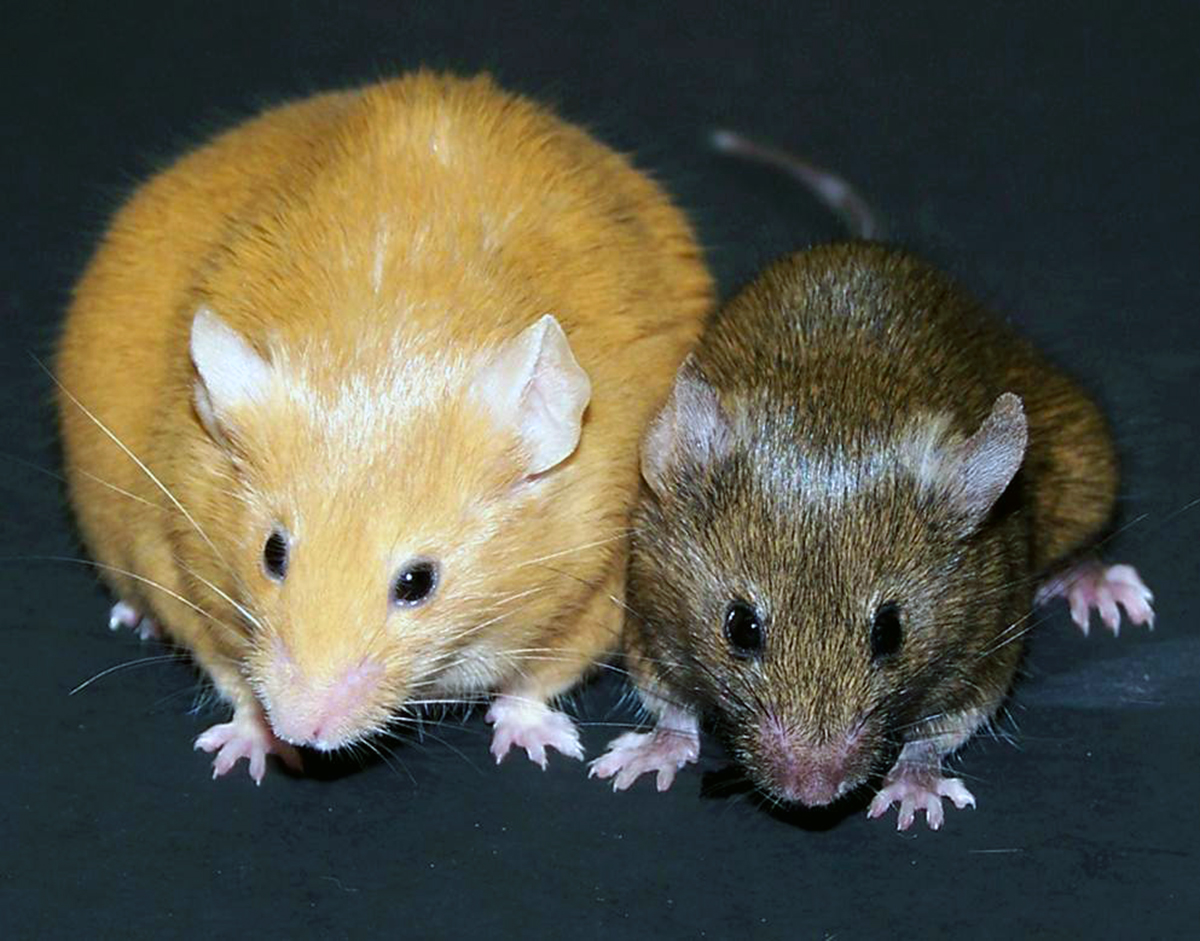
\includegraphics[height=8cm]{figs/Agouti.jpg}
\caption{\emph{Agouti} viable-yellow mutant mouse has yellow hair and is obese in comparison to a wild-type mouse. (https://upload.wikimedia.org/wikipedia/commons/4/4d/Agouti\_Mice.jpg)}
\label{fig:agouti}
\end{figure}




%two-parent designs: intercross & backcross
%mapping populations
%mice
% genotype data & hmm to infer 36-state genotype probabilities
%mapping genetic markers to measurable traits in MPP
%complex traits
%my test
%roadmap


\section{Designs for two-parent crosses}\label{sec:two-parent-designs}

Two widely used two-parent crosses are the ``backcross'' and the ``intercross''. We first discuss the backcross design (Figure~\ref{fig:backcross}). A backcross starts with mating between members of two inbred lines. The offspring of this mating event, termed the ``F$_1$'', or ``first filial'', generation then mate with members of one of the two parent lines. The experiment designers decide which line the female is chosen from and which line the F$_1$ mate with. Thus, there are a total of four possible backcrosses for any pair of inbred lines. 

As Figure~\ref{fig:backcross} illustrates, all backcross animals (generation ``BC'') have, for any locus, only two possible genotypes: heterozygote (AB) and homozygote (AA in the figure).
The F$_1$ generation is heterozygous at all loci (Figure~\ref{fig:backcross}) because 
they inherited one chromosome (of each pair) from each parent.
While meiotic crossovers may occur in the founder generation, these crossover events are
undetectable because the animals are inbred and, thus, have two identical copies
of DNA at every locus. This causes the F$_1$ subjects to be heterozygous at all positions
when genotyping with respect to the founder lines.
In fact, the F$_1$ may have identical single nucleotide marker alleles at some
positions, but, because one allele is inherited from each parent (and each inbred
founder line), we still call them ``heterozygous'' because, in terms of founder allele genotypes, they have the ``AB'' heterozygote genotype.

The meiotic crossovers that occur as the F$_1$ animals produce gametes often
are detectable because they result in ``BC'' generation animals that have individual
chromosomes that contain DNA from both founder lines. Due to the limited number
of crossovers in a single meiosis, the resulting ``BC'' generation subjects have
poor QTL mapping resolution.
This poor mapping resolution corresponds to the relatively large segments
of contiguous DNA, on average, that are inherited from, ultimately, the founder lines.








\begin{knitrout}
\definecolor{shadecolor}{rgb}{0.969, 0.969, 0.969}\color{fgcolor}\begin{figure}
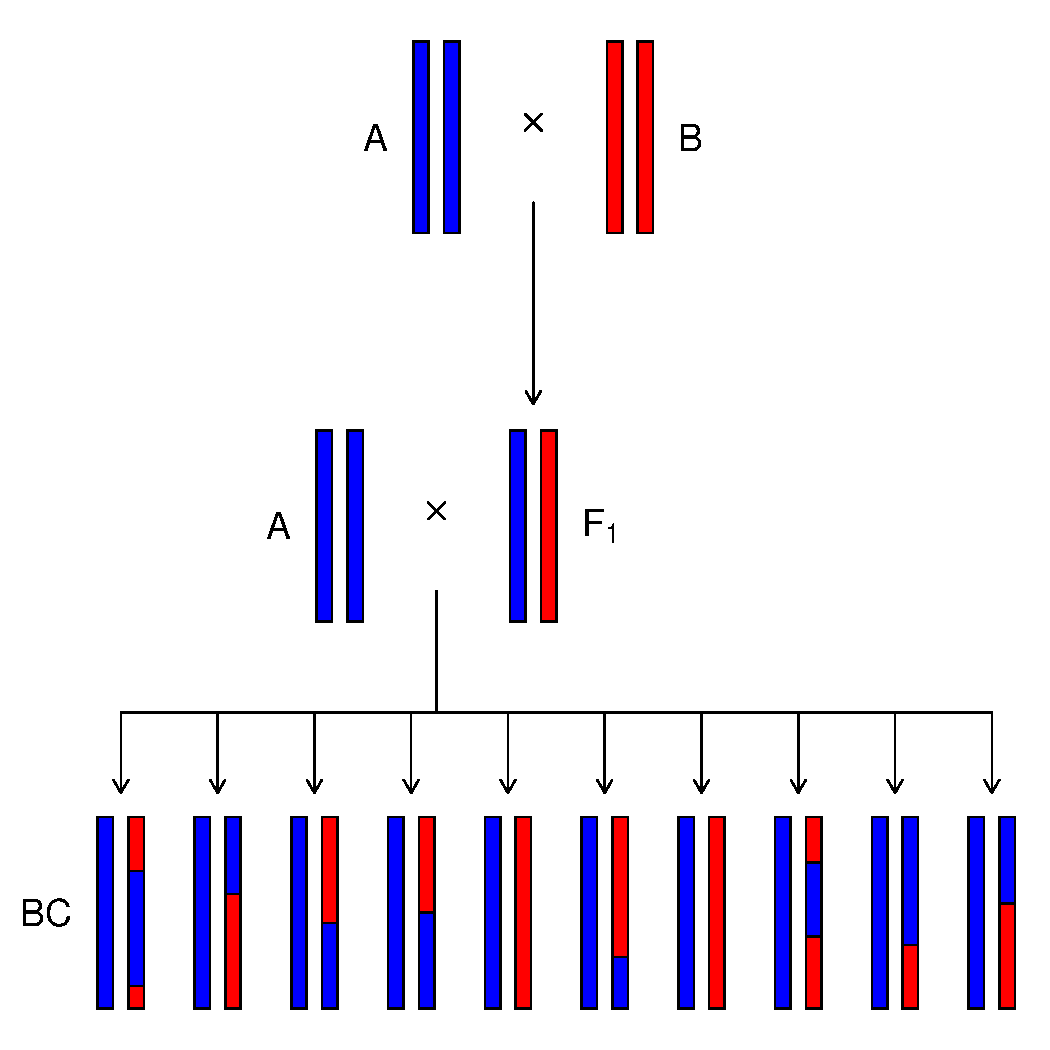
\includegraphics[width=\maxwidth,height=5in]{figure/backcross-1} \caption[Breeding scheme for a backcross]{Breeding scheme for a backcross. Each pair of autosomes represents a single subject.}\label{fig:backcross}
\end{figure}


\end{knitrout}


\begin{knitrout}
\definecolor{shadecolor}{rgb}{0.969, 0.969, 0.969}\color{fgcolor}\begin{figure}
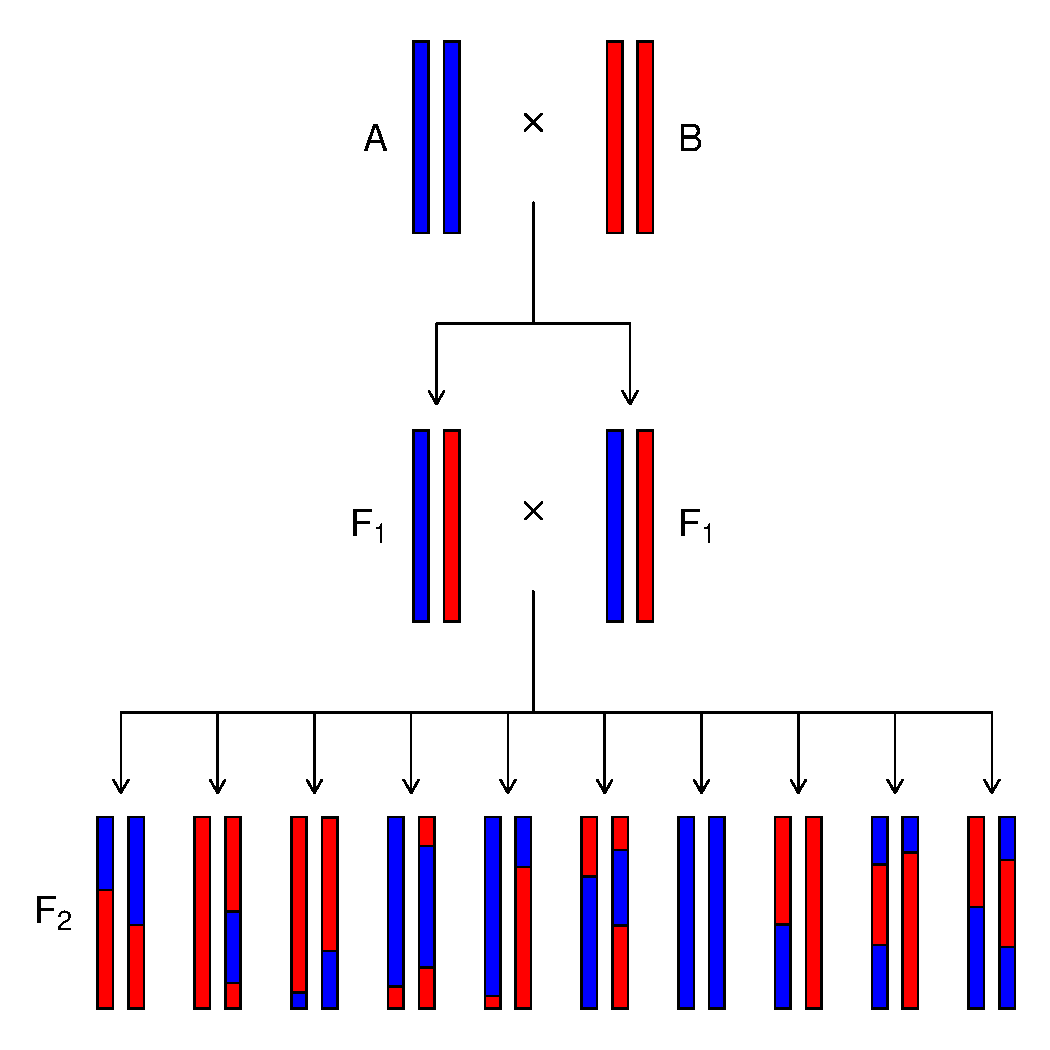
\includegraphics[width=\maxwidth,height=5in]{figure/intercross-1} \caption[Breeding scheme for an intercross]{Breeding scheme for an intercross. Each pair of autosomes represents a single subject.}\label{fig:intercross}
\end{figure}


\end{knitrout}


\section{QTL mapping in two-parent crosses}\label{sec:qtl-two-parent}

QTL mapping is a systematic, statistical approach to identifying genetic
loci where genetic variation affects variation in a measured trait.
We use the term ``locus'' to refer to a small, contiguous genomic region, often
several megabases in length. Standard inputs are genome-wide marker genotypes
for a collection of study subjects and a set of trait measurements on the same subjects.

% QTL scan (univariate)
A univariate QTL scan is a procedure to interrogate the entire genome for genetic
variants that affect a specified trait of interest.
One specifies a statistical model and calculates the
likelihood of the model parameters given the observed (trait and marker) data at each genomic position. 
After obtaining likelihoods for all markers, likelihood ratio test statistics are calculated
at every marker. The inputs for these calculations are the likelihoods from the model fits 
and the likelihood for the null model, which contains no genotype data.
The resulting likelihood ratios compare, for every marker, the null hypothesis that there is no 
QTL (at that marker) against the alternative that there is a QTL (at the specified marker).
In other words, one performs a likelihood ratio test for every marker across the genome.
Often this amounts to thousands of (statistically dependent) hypothesis tests.
One then uses a permutation test to determine a genome-wide critical value
for the likelihood ratio test statistic \citep{churchill1994empirical}.
Those loci for which the likelihood ratio test statistic is sufficiently large are declared QTL. 



In studies with sparse marker sets, one may use a strategy called ``interval mapping'' 
to combat what \citet{broman2009guide} call the ``missing data'' problem. 
The missing data problem refers to the fact that explicit genotyping occurs at
only a subset of genomic positions, \emph{i.e.}, those positions
occupied by the markers. In this sense, genotype data at all other
positions is ``missing''. As genotyping technologies have improved and
associated costs have decreased, dense marker sets are now available for
some multiparental populations. For example, the GigaMUGA single
nucleotide polymorphism (SNP) genotyping microarray \citep{morgan2015mouse} 
offers a dense marker set for studies of Diversity Outbred and 
Collaborative Cross mice.









%statistical challenges in QTL mapping
Two major statistical challenges are what \citet{broman2009guide} call 
the ``missing data'' problem and the ``model selection'' problem. 
The ``missing data'' problem arises in QTL studies because genotypes are obtained
at only select markers. In this sense, genotypes at positions between
markers are ``missing'' because they aren't explicitly measured
(Figure~\ref{fig:genoprob1}). Figure~\ref{fig:genoprob1} presents, for
one subject, a chromosome with genotyped markers at the tick marks.
The triangle represents a position at which we wish to know the genotype.
We now consider a strategy for inference of genotypes at intermarker positions.

\begin{figure}
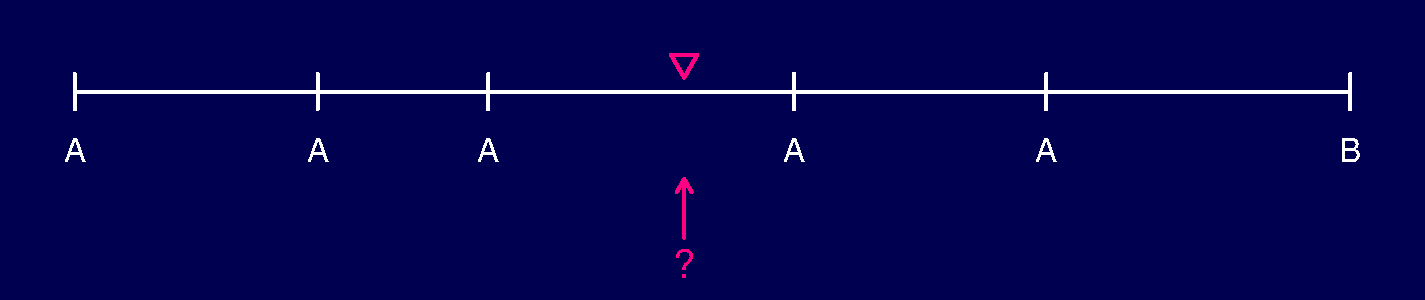
\includegraphics[width = \textwidth]{figs/genoprob1.pdf}
\caption{Inferring genotypes at an intermarker position.}\label{fig:genoprob1}
\end{figure}




A flexible framework for resolving the ``missing data'' problem involves use of a
hidden Markov model \citep{broman2009guide, broman2006use}. 
In this hidden Markov model, marker genotypes are observed random variables, 
while genotypes at intervening bases are unobserved random variables. 
Two sets of recursive equations, termed ``forward'' and ``backward'' equations,
enable efficient calculation of genotype probabilities
(conditional on the observed marker genotypes) \citep{baum1970maximization}.
We discuss inference methods for genotype probabilities in Appendix~\ref{sec:stat-primer}.




% model form - linear regression
A QTL analysis involves choosing a statistical model to be fitted at every marker. 
As in any statistical modeling, there is not one best model selection procedure.
One needs to decide which main effects and interactions are needed.
Also, one often transforms the trait values to achieve approximate normality before performing the QTL scan. 

Many investigators consider multiple models before performing a QTL scan.
For simplicity, one may choose a linear model that contains additive effects for
the  minor allele count (0, 1 or 2) at a given marker (Equation~\ref{eq:uni-2-parent}) \citep{martinez1992estimating,haley1992simple}.

\begin{equation}
\text{trait} = \text{mean for major allele homozygotes} + \text{(minor allele count)}\text{(minor allele effect)} + \text{random error}
\label{eq:uni-2-parent}
\end{equation}

Assuming that the random errors are normally distributed (and independent with common
variance $\sigma^2$), one may use the statistical technique called ``ordinary least squares''
to fit the model and to solve for $\hat b$ and $\hat \sigma^2$.
In ``ordinary least squares'', one solves for the set of parameter values that
minimize the residual sum of squares.
In the above equation, our two parameters are the minor allele effect and
the random error variance. The residual sum of squares is an expression that
tells us how far each observed data point is from its predicted value for a
set of specified parameter values. Equation~\ref{eq:rss} defines residual
sum of squares for a univariate QTL analysis.

\begin{equation}
\text{residual sum of squares} = \sum_{\text{subjects}}\left(\text{observed trait value} - \text{fitted trait value}\right)^2\label{eq:rss}
\end{equation}

I define the fitted trait value, $\hat y$, for a single subject with Equation~\ref{eq:fitted-values}. 
The character tilde above a quantity denotes its least squares estimate. 

\begin{equation}
\tilde y = \tilde{\text{(fitted trait value)}} = 
\label{eq:fitted-values}
\end{equation}



\section{Testing pleiotropy in two-parent crosses}\label{sec:pleiotropy-two-parent}

In anticipation that multivariate mapping of correlated traits would enhance statistical
power to detect QTL and would improve precision of QTL positions,
both \citet{jiang1995multiple} and \citet{korol1995interval} developed
multivariate interval mapping procedures for two-parent crosses. 
Among the novel methods from \citet{jiang1995multiple} is a test of pleiotropy vs separate QTL.
They explain that such a test is useful when two traits map to a single genomic region.
The question then arises ``do the two traits associate with the same locus, or do they associate with separate loci''?

If both traits associate with the same locus, then that locus is called ``pleiotropic''. If the two traits associate with separate loci, then we say that there are separate QTL (one for each trait). 
In the development of their test of pleiotropy v separate QTL, \citet{jiang1995multiple} model
the multivariate trait as the sum of a linear function of the genotypes and a random error term. They assume that the traits matrix is related to the genotype data through Equation~\ref{eq:jz95}.


\begin{equation}
vec(Y) = Xvec(B) + vec(E)\label{eq:jz95}
\end{equation}


In Equation~\ref{eq:jz95}, $Y$ is a $n$ by $2$ matrix of trait values (with each row being one subject and each column being one trait)
, $X$ is a $2n$ by $4$ block-diagonal matrix containing genotype data for two positions, and $B$ is a $4$ by $1$ matrix of allele effects.
The random error is assumed to follow a normal distribution with mean zero and a positive variance.
\citet{jiang1995multiple} also incorporate additional terms to model dominant effects and to
control for residual genetic variation.
To simplify model specification, we forego inclusion of dominant terms
and additional markers for controlling residual
genetic variation.
Extensions of our model and software to accommodate dominance effects are straightforward.


\citet{jiang1995multiple} use a mixture model to relate genotypes to phenotypes. 
They observe that the there are 9 possible ordered pairs of genotypes for two markers in a F$_2$ population, since each marker has one of three genotypes (AA, AB, BB).
They thus approach the problem as one with a 9-state mixture model. 
They provide the equations needed for an expectation-conditional maximization
(ECM) algorithm for fitting the mixture model.
They use a chi-square distribution with one degree of freedom as the
null distribution of the test statistic. 

Further investigations by \citet{jiang1995multiple} with simulations revealed
reasonable behavior of the hypothesis test under the specified conditions. 
They learned that dense marker coverage tends to aid in distinguishing pleiotropy
from separate QTL. \todo[inline]{IS THIS TRUE?? look back at JZ 1995's simulations. How did they examine power and type I error rates? Do they examine univariate LOD strength when considering power? What about interlocus distance? AND KAO 2000}










They use a computational algorithm called ``expectation - conditional maximization'' to find these values. 
ECM is an iterative algorithm. 
The user inputs starting values for the parameters and the algorithm changes them one at a
time until the change in log likelihood between successive iterations is sufficiently small.
The algorithm is then said to have ``converged''. 
The final iteration’s parameter values are treated as those that maximize the likelihood.


\citet{jiang1995multiple}, in the context of their multivariate QTL mapping methods, 
describe a test of pleiotropy vs. separate QTL. 
They formulate a test in which the null hypothesis
is pleiotropy while the the alternative hypothesis is separate QTL.
In other words, they consider the case in which the two traits map to the same locus
(pleiotropy) as a special case of the more general setting (separate QTL)
in which the two traits may or may not map to the same locus.

In statistical terminology, one would say that the parameter space is restricted under the null hypothesis. Here, the parameter space is the collection of ordered pairs of markers in the genomic region of interest. The restriction of that collection under pleiotropy corresponds to limiting consideration to only those ordered pairs that have both traits mapping to a single locus. 

We illustrate these ideas in a drawing of a two-dimensional grid (Figure~\ref{fig:encircle}). Each point in the grid corresponds to an ordered pair of markers. Along the horizontal axis are the markers for the first component of the ordered pair; the second component of the ordered pair is indicated by the vertical axis. The red points correspond to those that are considered under the pleiotropy hypothesis. Under the alternative hypothesis, all grid points are considered. 




\begin{knitrout}
\definecolor{shadecolor}{rgb}{0.969, 0.969, 0.969}\color{fgcolor}\begin{figure}
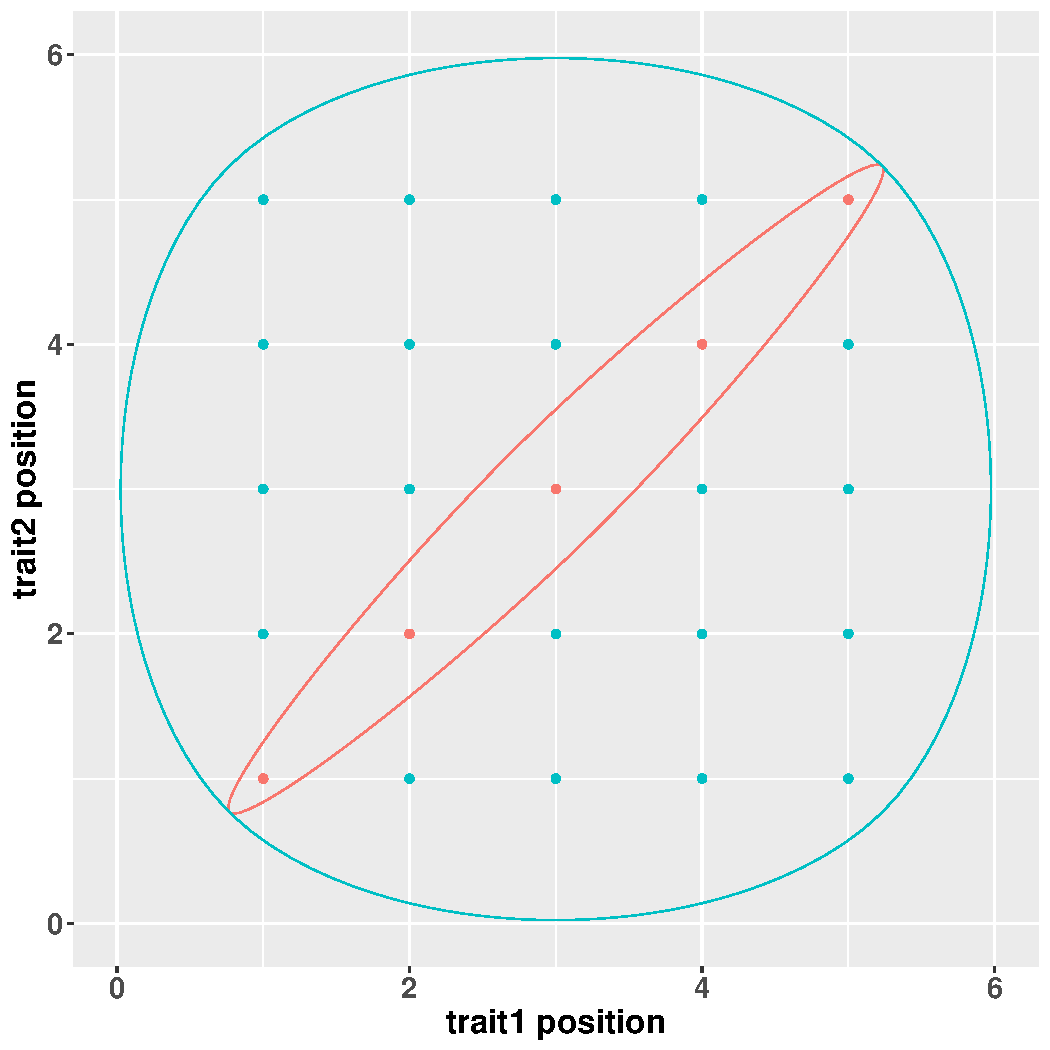
\includegraphics[width=4in,height=4in]{figure/encircle-1} \caption[Two-dimensional grid of ordered pairs of markers]{Two-dimensional grid of ordered pairs of markers.}\label{fig:encircle}
\end{figure}


\end{knitrout}



\citet{jiang1995multiple} then calculate the likelihoods of the two models
(that under the hypothesis of pleiotropy and that under the hypothesis of separate QTL)
at each ordered pair of putative loci in the genomic region of interest.
The likelihood ratio test statistic is the logarithm of the ratio of the maximum
of the likelihoods under pleiotropy to the maximum of the likelihoods under
the separate QTL hypothesis. 

\citet{jiang1995multiple} determined p-values for their test statistics by comparing
them to a chi-squared distribution with 1 degree of freedom. 





\section{Designs for multiparental populations and Diversity Outbred mice}\label{sec:mpp-designs}

Near the turn of the century, geneticists sought a mammalian gene mapping resource 
that could be used for study of a wide variety of quantitative traits. 
The magnitude of such an undertaking required a collaborative, community-supported
approach \citep{de2014genetics}. Scientists conceived of the Diversity Outbred (DO)
mouse population as such a high-resolution gene mapping resource.
They elected to seed the population with partially inbred progenitors of the
Collaborative Cross lines. The Collaborative Cross mating design started with
mice from eight inbred lines: A/J, C57BL/6J, 129S1/SvImJ,
NOD/ShiLtJ, NZO/HILtJ, CAST/EiJ, PWK/PhJ, WSB/EiJ. Three of these lines, CAST/EiJ, PWK/PhJ, and WSB/EiJ, are wild-derived. Together, the three wild-derived lines contribute 

The designers of the Collaborative Cross used a ``multi-funnel'' mating scheme to generate
mice with DNA from all eight founder lines over the course of 3 generations.
The term ``funnel'' refers to the design for the first 3 mating generations in which the
DNA from eight founder lines ``funnels'' into animals that have DNA from all eight founders.
For example, in one funnel, mating pairs are: A x B, C x D, E x F, and G x H in the first generation (Figure~\ref{fig:ri8}).
AB offspring would then mate with CD offspring and EF offspring would mate with GH mice.
Finally, the ABCD mice would mate with the EFGH mice to create a generation of mice that
contain genetic material from all eight inbred founder lines.
Subsequent generations of inbreeding resulted in multiple inbred lines for the Collaborative Cross.

\begin{knitrout}
\definecolor{shadecolor}{rgb}{0.969, 0.969, 0.969}\color{fgcolor}\begin{kframe}


{\ttfamily\noindent\bfseries\color{errorcolor}{\#\# Error in gzfile(file, "{}wb"{}): cannot open the connection}}\end{kframe}\begin{figure}
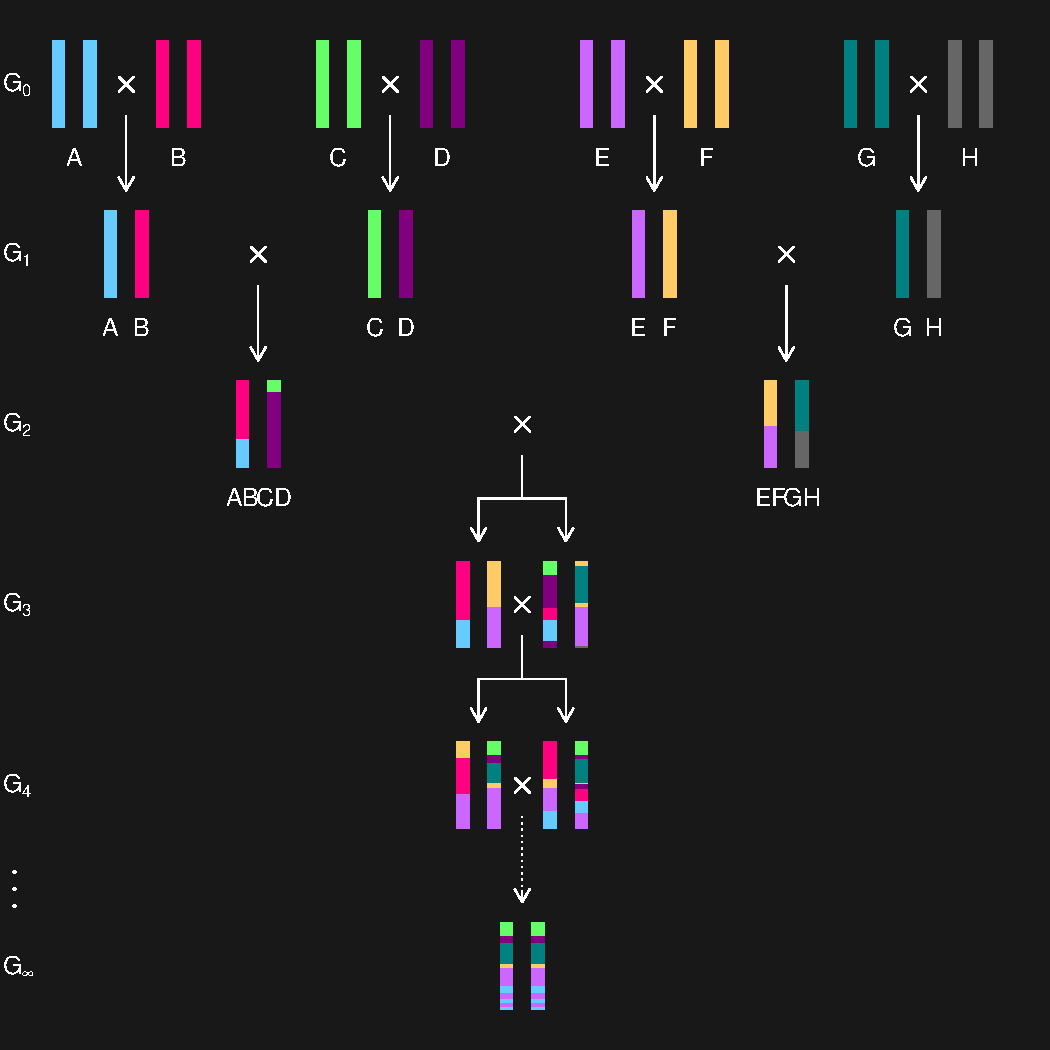
\includegraphics[width=\maxwidth]{figure/ri8-1} \caption[Schematic for a single funnel in the Collaborative Cross breeding design]{Schematic for a single funnel in the Collaborative Cross breeding design.}\label{fig:ri8}
\end{figure}


\end{knitrout}




The designers of the Diversity Outbred population started with \todo[inline]{get number of mice and from which generations}

Due to the breeding scheme, each Diversity Outbred mouse is a highly heterozygous mosaic of 
founders' DNA (Figure)\todo{add figure with mosaics over multiple generations here}. 
With each generation, the Diversity Outbred mice accumulate meiotic recombinations. 
This is because each mouse inherits DNA from its parents, and each meiosis provides opportunities for recombinations. \todo[inline]{need to explain this better. How does Andrew explain it in his thesis?}

The cumulative effect of recombinations over many generations of outbreeding is to create mice whose DNA mosaic contains smaller and smaller contiguous pieces from each founder line. 

The Diversity Outbred mice enable high-resolution QTL mapping \citep{gatti2014quantitative}. One factor that contributes to high-resolution mapping is the ability to infer the founder line from which each marker's DNA arose. 




\section{QTL mapping in Diversity Outbred mice}\label{sec:do-qtl}

QTL mapping in Diversity Outbred mice, like that in mice from two-parent crosses, is a multi-step procedure: 1. data acquisition, 2. inference of missing genotypes, and 3. modeling phenotypes as a function of genotypes. Data acquisition involves measurement of phenotypes and, at specified genetic markers, termed ``single nucleotide polymorphism'' or SNP markers, measurement of two-allele genotypes. Often, the SNP marker genotypes are obtained by use of a microarray, such as the GigaMUGA SNP microarray \citep{morgan2015mouse}. 

The next step, missing genotypes inference, is needed because of the ``missing data problem'' \citep{broman2009guide}. It takes as input the two-allele genotypes at the measured SNP markers. An expectation maximization algorithm \citep{dempster1977maximum} for a hidden Markov model, developed by \citet{broman2012haplotype} and \citet{broman2012genotype} and implemented in the \texttt{qtl2} R package \citep{broman2019rqtl2}, outputs 36-state genotype probabilities for all nuclear autosomal markers and pseudomarkers. Pseudomarkers, as we use the term, are arbitrary nucleotide bases at which the researcher wants 36-state genotype probabilities. Finally, we collapse the 36-state genotype probabilities to eight founder allele dosages at each marker. This last step is optional, but often helpful, because the simplified models require specification of fewer parameters. We then treat the founder allele dosages as known quantities in subsequent steps. 

% model form - connecting genotype to phenotype

After inferring founder allele dosages, we address the second major statistical challenge of 
QTL mapping: the ``model selection'' problem \citep{broman2009guide}.
Linear regression is widely used because of its ease of implementation,
computational speed, and interpretability of results.
A genetically ``additive'' linear model, in which we assume a linear relationship between
a trait's values and each founder allele's dosage, is the default model.
\citep{gatti2014quantitative,broman2019rqtl2}.
The R package \texttt{qtl2} provides a straightforward user
interface to include covariates and interaction terms in the linear model \citep{broman2019rqtl2}.




% model form - random effects incorporation & relatedness
% First, relatedness
Relatedness is one issue that arises in the Diversity Outbred mice that is not a major concern in 
two-parent crosses. Due to the complexity of the breeding design, Diversity Outbred mice
have 
complicated pairwise relationships. A given study cohort may include pairs of first
cousins, parent-offspring pairs, grandparent-grandchild pairs, second cousin pairs, and others.
Contrasting this with the two-parent backcross (Figure~\ref{fig:backcross}) and
intercross (Figure~\ref{fig:intercross}) designs, we see in the backcross that
average relatedness between any two members of the BC generation is equal to the same, shared value.
One measure of relatedness is the probability of identity by state, \emph{i.e.}, the
probability that a randomly chosen allele from one subject is identical to a randomly chosen
allele of the second subject. Measured in terms of the probability that a randomly chosen allele
from one subject is identical to a randomly chosen allele of a second subject, we note that
this probability of identity by state is $\frac{5}{8}$ in the backcross. F$_2$ subject pairs in an intercross, likewise, have a single, shared average relatedness, with an identity by state probability of $\frac{1}{2}$.

Because relatedness can confound genotype-phenotype associations \citep{yang2014advantages}, researchers have developed methods to account for relatedness in their statistical models. One popular approach involves use of a polygenic random effect in the statistical model \citep{kang2008efficient}. The addition of a random effect to a model with fixed (\emph{i.e.}, nonrandom) effects results in what statisticians call a ``linear mixed effects model''. 

\section{Benefits of a pleiotropy test in multiparental populations}\label{sec:pleiotropy-mpp}








%%% CHAPTER 1 End
%%%%%%%%%%%%%%%%%
%%% chapter 2 start
\chapter{Methods development}


\section{Introduction}

Complex trait studies in multiparental populations present new
challenges in statistical methods and data analysis. Among these is
the development of strategies for multivariate trait analysis. The
joint analysis of two or more traits allows one to address additional
questions, such as whether two traits share a single pleiotropic
locus.




Previous research addressed the question of pleiotropy vs.\ separate
QTL in two-parent crosses.
\citet{jiang1995multiple} developed a likelihood
ratio test for pleiotropy vs.\ separate QTL for a pair of traits.
Their approach assumed that each trait was affected by a single QTL.
Under the null hypothesis, the two traits were affected by a common
QTL, and under the alternative hypothesis the two traits were affected
by distinct QTL.
\citet{knott2000multitrait} used linear regression to develop a fast
approximation to the test of \citet{jiang1995multiple}, while
\citet{tian2016dissection} used the methods from
\citet{knott2000multitrait} to dissect QTL hotspots in a F$_2$
population.


Multiparental populations, such
as the Diversity Outbred (DO) mouse population \citep{churchill2012diversity}, enable high-precision
mapping of complex traits \citep{de2014genetics}. The DO
mouse population began with progenitors of the Collaborative
Cross (CC) mice \citep{churchill2004collaborative}
Each DO mouse is a highly heterozygous genetic mosaic
of alleles from the eight CC founder lines. Random
matings among non-siblings have maintained the DO
population for more than 23 generations \citep{chesler2016diversity}.

Several limitations of previous pleiotropy vs.\ separate QTL tests
prevent their direct application in multiparental populations. First,
multiparental populations can have complex patterns of relatedness
among subjects, and failure to account for these patterns of
relatedness may lead to spurious results \citep{yang2014advantages}.
Second, previous tests allowed for only two founder lines
\citep{jiang1995multiple}. Finally, \citet{jiang1995multiple} assumed
that the null distribution of the test statistic follows a chi-square
distribution.

We developed a pleiotropy vs.\ separate QTL test for two traits in
multiparental populations. Our test builds on research that
\citet{jiang1995multiple}, \citet{knott2000multitrait},
\citet{tian2016dissection}, and \citet{zhou2014efficient} initiated.
Our innovations include the accommodation of $k$ founder alleles per
locus (compared to the traditional two founder alleles per locus) and
the incorporation of multivariate polygenic random effects to account
for relatedness. Furthermore, we implemented a parametric bootstrap to
calibrate test statistic values \citep{efron1979,tian2016dissection}.

Below, we describe our likelihood ratio test for pleiotropy vs.\
separate QTL. In simulation studies, we find that it is slightly
conservative, and that it has power to detect two separate loci when
the univariate LOD peaks are strong. We further illustrate our
approach with an application to data on a pair of behavior traits in
a population of 261 DO mice \citep{logan2013high,recla2014precise}.
We find modest evidence for distinct QTL in a 2.5-cM region on mouse
Chromosome 8.


\section{Methods}
\label{sec:materials:methods}

Our strategy involves first identifying two traits that map to a common
genomic region. We then perform a two-dimensional, two-QTL scan over
the genomic region, with each trait affected by one QTL of varying
position. We identify the QTL position that maximizes the likelihood
under pleiotropy (that is, along the diagonal where the two QTL are at
a common location), and the ordered pair of positions that maximizes
the likelihood under the model where the two QTL are allowed to be
distinct. The logarithm of the ratio of the two likelihoods is our
test statistic. We calibrate this test statistic with a parametric
bootstrap.

\section{Data structures}

The data consist of three objects. The first is an $n$ by $k$ by $m$
array of allele probabilities for $n$ subjects with $k$ alleles and
$m$ marker positions on a single chromosome [derived from the observed
SNP genotype data by a hidden Markov model; see
\citet{broman2019rqtl2}]. The second object is an $n$ by 2 matrix of
phenotype values. Each column is a phenotype and each row is a
subject. The third object is an $n$ by $c$ matrix of covariates, where
each row is a subject and each column is a covariate.

One additional object is the genotype-derived kinship matrix, which is
used in the linear mixed model to account for population structure. We
are focusing on a defined genomic interval, and we prefer to use a
kinship matrix derived by the ``leave one chromosome out'' (LOCO)
method \citep{yang2014advantages}, in which the kinship matrix is
derived from the genotypes for all chromosomes except the chromosome
under test.




\subsection{Statistical Models}

Focusing on a pair of traits and a particular genomic region of
interest, the next step is a two-dimensional, two-QTL
scan \citep{jiang1995multiple}. We consider two QTL with each
affecting a different trait, and consider all possible pairs of
locations for the two QTL. For each pair of positions, we fit
the multivariate linear mixed effects model defined in Equation
\ref{eqn:model1}. Note that we have
assumed an additive genetic model throughout our analyses, but
extensions to design matrices that include dominance are
straightforward.


\begin{equation}
vec(Y) = X vec(B) + vec(G) + vec(E)
\label{eqn:model1}
\end{equation}
where $Y$ is the $n$ by $2$ matrix of phenotypes values;
$X$ is a $2n$ by $2(k + c)$
matrix that contains the $k$ allele probabilities for the two QTL
positions and the $c$
covariates in diagonal blocks; $B$ is a $(k + c)$ by $2$ matrix of
allele effects and covariate effects; $G$ is a $n$ by $2$ matrix of
random effects; and $E$ is a $n$ by $2$ matrix of random errors. $n$
is the number of mice. The `vec' operator stacks columns from a matrix
into a single vector. For example, a 2 by 2 matrix inputted to `vec'
results in a vector with length 4. Its first two entries are the
matrix's first column, while the third and fourth entries are the
matrix's second column.


We also impose distributional assumptions on $G$ and $E$:

\begin{equation}
G \sim MN_{n x 2}(0, K, V_g)
\label{eqn:model2}
\end{equation}

and

\begin{equation}
E \sim MN_{nx2}(0, I, V_e)
\label{eqn:model3}
\end{equation}
where $MN_{n x 2}(0, V_r, V_c)$ denotes the matrix-variate ($n$ by 2)
normal distribution with mean being the $n$ by $2$ matrix with all
zero entries and row covariance $V_r$ and column covariance $V_c$. We
assume that $G$ and $E$ are independent.


\subsection{Parameter inference and log likelihood calculation}

Inference for parameters in multivariate linear mixed effects models
is notoriously difficult and can be computationally intense
\citep{meyer1989restricted,meyer1991estimating}. Thus, we estimate
$V_g$ and $V_e$ under the null hypothesis of no QTL, and then take
them as fixed and known in our two-dimensional, two-QTL genome scan.
We use restricted maximum likelihood methods to fit the
model:

\begin{equation}
vec(Y) = X_0vec(B) + vec(G) + vec(E)
\label{model}
\end{equation}
where $X_0$ is a $2n$ by $2(c + 1)$ matrix whose first column of each
diagonal block in $X_0$ has all entries equal to one (for an intercept); the remaining
columns are the covariates.

We draw on our R implementation \citep{gemma2} of the
GEMMA algorithm for fitting a multivariate linear mixed effects model
with expectation-maximization \citep{zhou2014efficient}. We use
restricted maximum likelihood fits for the variance components $V_g$
and $V_e$ in subsequent calculations of the generalized least squares
solution $\hat B$.

\begin{equation}
    \hat B = (X^T\hat\Sigma^{-1}X)^{-1}X^T\hat\Sigma^{-1}vec(Y)
\end{equation}

\noindent where

\begin{equation}
    \hat\Sigma = \hat V_g \otimes K + \hat V_e \otimes I_n
    \label{cov}
\end{equation}

\noindent where $\otimes$ denotes the Kronecker product, $K$ is the
kinship matrix, and $I_n$ is a n by n
identity matrix. We then calculate the log likelihood for a normal
distribution with mean $X vec(\hat B)$ and covariance $\hat \Sigma$
that depends on our estimates of $V_g$ and $V_e$ (Equation \ref{cov}).

\subsection{Pleiotropy vs.\ separate QTL hypothesis testing framework}

Our test applies to two traits considered simultaneously. Below,
$\lambda_1$ and $\lambda_2$ denote putative locus positions for traits
one and two. We quantitatively state the competing hypotheses for our
test as:

\begin{eqnarray}
H_0: \lambda_1 = \lambda_2 \nonumber\\
H_A: \lambda_1 \neq \lambda_2
\label{eqn:hypotheses}
\end{eqnarray}

\noindent Our likelihood ratio test statistic is:

\begin{equation}
\text{LOD} = \log_{10} \left[ \frac{\max_{\lambda_1, \lambda_2} L(B, \Sigma, \lambda_1, \lambda_2)}{
    \max_\lambda L(B, \Sigma, \lambda, \lambda)} \right]
\label{eqn:test-statistic}
\end{equation}
where $L$ is the likelihood for fixed QTL positions,
maximized over all other parameters.

\subsection{Visualizing profile LOD traces}

The output of the above analysis is a two-dimensional log$_{10}$ likelihood
surface. To visualize these results, we followed an innovation of \citet{zeng2000genetic} and
\citet{tian2016dissection}, and plot three traces: the results along the
diagonal (corresponding to the null hypothesis of pleiotropy), and
then the profiles derived by fixing one QTL's position
and maximizing over the other QTL's position.

We define the LOD score for our test:

\begin{equation}
\text{LOD}(\lambda_1, \lambda_2) = ll_{10}(\lambda_1, \lambda_2) - \max ll_{10}(\lambda, \lambda)
\label{eq:lodpvl}
\end{equation}
where $ll_{10}$ denotes log$_{10}$ likelihood.

We follow \citet{zeng2000genetic} and \citet{tian2016dissection} in
defining profile LOD by the equation

\begin{equation}
\text{profile LOD}_1(\lambda_1) = \max_{\lambda_2}\text{LOD}(\lambda_1, \lambda_2)
\label{eq:profilelod}
\end{equation}
We define profile LOD$_2(\lambda_2)$ analogously.
The maximum value for the profile LOD$_1$
profile LOD$_2$ traces are the same and are non-negative, and give the
overall LOD test statistic.

We construct the pleiotropy trace by calculating the log-likelihoods
for the pleiotropic models at every position.

\begin{equation}
LOD_{p}(\lambda) = ll_{10}(\lambda, \lambda) - \max ll_{10}(\lambda, \lambda)
\label{eq:lodp}
\end{equation}
By definition, the maximum value for this pleiotropy trace
is zero.






\subsection{Bootstrap for test statistic calibration}

We use a parametric bootstrap to calibrate our test statistic
\citep{efron1979}. While \citet{jiang1995multiple} used quantiles of a
chi-squared distribution to determine p-values, this does not account
for the two-dimensional search over QTL positions.
We follow the approach of \citet{tian2016dissection}, and identify
the maximum likelihood estimate of the QTL position under the null
hypothesis of pleiotropy.
We then use the inferred model parameters under that model and with
the QTL at that position to simulate bootstrap data sets according to
the model in equations \ref{eqn:model1}--\ref{eqn:model3}.
For each of $b$ bootstrap data sets, we
perform a two-dimensional QTL scan (over the genomic region of
interest) and derive the test
statistic value. We treat these $b$ test statistics as the
empirical null distribution, and calculate a p-value as the
proportion of the $b$ bootstrap test statistics that equal or exceed
the observed one, with the original data,
$p = \# \{ i:\text{LOD}^*_i \geq \text{LOD}\} / b$
where $\text{LOD}_i^*$ denotes the LOD score for the $i$th bootstrap
replicate and LOD is the observed test statistic.



\subsection{Data \& Software Availability}

Our methods have been implemented in an R package, \texttt{qtl2pleio},
available at GitHub:

\href{https://github.com/fboehm/qtl2pleio}{https://github.com/fboehm/qtl2pleio}

\noindent Custom R code for our analyses and simulations are at GitHub:

\href{https://github.com/fboehm/qtl2pleio-manuscript-clean}{https://github.com/fboehm/qt2pleio-manuscript-clean}

\noindent The data from \citet{recla2014precise} and
\citet{logan2013high} are available at the Mouse Phenome Database:

\href{https://phenome.jax.org/projects/Chesler4}{https://phenome.jax.org/projects/Chesler4} and \href{https://phenome.jax.org/projects/Recla1}{https://phenome.jax.org/projects/Recla1}.

\noindent They are also available in R/qtl2 format at
\href{https://github.com/rqtl/qtl2data}{https://github.com/rqtl/qtl2data}.




\section{Simulation studies}

We performed two types of simulation studies, one for type I error
rate assessment and one to characterize the power to detect separate
QTL. To simulate traits, we specified $X$, $B$, $V_g$, $K$, and $V_e$
matrices (Equations \ref{eqn:model1}--\ref{eqn:model3}). For both we
used the allele probabilities from a single genomic region derived
empirically from data for a set of 479 Diversity Outbred mice from
\citet{keller2018genetic}.

\subsection{Type I error rate analysis}

To quantify type I error rate ({\em i.e.}, false positive rate), we
simulated 400 pairs of traits for each of eight sets of parameter
inputs (Table~\ref{table-typeI}). We used a $2^3$ factorial
experimental design with three factors: allele effects difference,
allele effects partitioning, and genetic correlation, \textit{i.e.},
the off-diagonal entry in the 2 by 2 matrix $V_g$.

\begin{table}
\begin{center}
  \caption{Type I error rates for all runs in our $2^3$
    experimental design. We set (marginal) genetic variances
    (\emph{i.e.}, diagonal elements of $V_g$) to 1 in all runs. $V_e$
    was set to the 2 by 2 identity matrix in all runs. We used allele
    probabilities at a single genetic marker to simulate traits for
    all eight sets of parameter inputs. In the
    column ``Allele effects partitioning'', ``ABCD:EFGH'' means that lines
    A--D carry one QTL allele while lines E--H carry the other allele.
    ``F:ABCDEGH'' means the QTL has a private allele in strain F.}
  \label{table-typeI}

  \bigskip

\small
  \begin{tabular}{ c | c | c | c | c}
    \hline
    Run & $\Delta$(Allele effects) & Allele effects partitioning & Genetic correlation & Type I error rate \\ \hline
    1 & 6 & ABCD:EFGH & 0 & 0.032\\
    2 & 6 & ABCD:EFGH & 0.6 & 0.035\\
    3 & 6 & F:ABCDEGH & 0 & 0.040\\
    4 & 6 & F:ABCDEGH & 0.6 & 0.045\\
    5 & 12 & ABCD:EFGH & 0 & 0.038\\
    6 & 12 & ABCD:EFGH & 0.6 & 0.042\\
    7 & 12 & F:ABCDEGH & 0 & 0.025\\
    8 & 12 & F:ABCDEGH & 0.6 & 0.025\\
    \hline
  \end{tabular}
\end{center}
  \end{table}

We chose two strong allele effects difference values, 6 and 12. These
ensured that the univariate phenotypes mapped with high LOD scores to
the region of interest. For the allele partitioning factor, we used
either equally frequent QTL alleles, or a private allele in the CAST
strain (F). For the residual genetic correlation (the off-diagonal
entry in $V_g$), we considered the values 0 and 0.6. The marginal
genetic variances (\textit{i.e.}, the diagonal entries in $V_g$) for
each trait were always set to one.

We performed 400 simulation replicates per set of parameter inputs,
and each used $b = 400$ bootstrap samples. For each bootstrap sample, we calculated the
test statistic (Equation \ref{eqn:test-statistic}). We then compared
the test statistic from the simulated trait against the empirical
distribution of its 400 bootstrap test statistics. When the simulated
trait's test statistic exceeded the 0.95 quantile of the empirical
distribution of bootstrap test statistics, we rejected the null
hypothesis. We observed that the test is slightly conservative over
our range of parameter selections (Table~\ref{table-typeI}), with
estimated type I error rates $<$ 0.05.


\subsection{Power analysis}

We also investigated the power to detect the presence of two
distinct QTL. We used a 2 $\times$ 2 $\times$ 5 experimental design, where our
three factors were allele effects difference, allele effects
partitioning, and inter-locus distance. The two levels of allele
effects difference were 1 and 2. The two levels of allele effects
partitioning were as in the type I error rate studies, ABCD:EFGH and
F:ABCDEGH (Table~\ref{table-letters}). The five levels of interlocus
distance were 0, 0.5, 1, 2, and 3 cM. $V_g$ and $V_e$ were both set to
the 2 by 2 identity matrix in all power study simulations.

We simulated 400 pairs of traits per set of parameter inputs. For
each simulation replicate, we calculated the likelihood ratio test
statistic. We then applied our parametric bootstrap to calibrate the
test statistics. For each simulation replicate, we used $b = 400$ bootstrap
samples. Because the bootstrap test statistics within a single set of
parameter inputs followed approximately the same distribution, we
pooled the $400 * 400 = 160,000$ bootstrap samples per set of
parameter inputs and compared each test statistic to the empirical
distribution derived from the 160,000 bootstrap samples. However, for
parameter inputs with interlocus distance equal to zero, we didn't
pool the 160,000 bootstrap samples; instead, we proceeded by
calculating power (\textit{i.e.}, type I error rate, in this case), as we did in the
type I error rate study above.

\begin{figure}
\includegraphics[width = \textwidth]{../qtl2pleio-manuscript/R/power-curves.eps}
\caption{Pleiotropy vs.\ separate QTL power curves for each of four
  sets of parameter settings. Factors that differ among the four
  curves are allele effects difference and allele partitioning. Red denotes high allele effects difference, while black is the low allele effects difference. Solid line denotes the even allele partitioning (ABCD:EFGH), while dashed line denotes the uneven allele partitioning (F:ABCDEGH).}
\label{fig:power}
\end{figure}

We present our power study results in Figure~\ref{fig:power}.
Power increases as interlocus distance increases. The top two curves
correspond to the case where the QTL effects are largest. For each value
for the QTL effect, power is greater when the QTL alleles are equally
frequent, and smaller when a QTL allele is private to one strain. One
can have high power to detect that the two traits have distinct QTL
when they are separated by $>$ 1~cM and when the QTL have large effect.


\section{Application}
\label{sec:app}

To illustrate our methods, we applied our test to data from
\citet{logan2013high} and \citet{recla2014precise}, on 261 DO mice
measured for a set of behavioral phenotypes.
\citet{recla2014precise} identified \textit{Hydin} as the gene that
underlies a QTL on Chromosome 8 at 57 cM for the ``hot plate latency''
phenotype (a measure of pain tolerance). The phenotype ``percent time in light''
in a light-dark box (a measure of anxiety) was
measured on the same set of mice \citep{logan2013high} and also shows a QTL near
this location, which led us to ask whether the same locus affects both traits.
The two traits show a correlation of $-0.15$ (Figure~\ref{fig:scatter}).

QTL analysis with the LOCO method, and using sex as an additive
covariate, showed multiple suggestive QTL for each
phenotype (Figure~\ref{fig:genomewide10-22}; Table~\ref{table-peaks}). For our investigation of
pleiotropy, we focused on the interval 53--64~cM on Chromosome 8.
The univariate QTL results for this region are shown in
Figure~\ref{fig:chr8-lod}.

\begin{figure}
\includegraphics[width = \textwidth]{../qtl2pleio-manuscript/Rmd/chr8-lods.eps}
\caption{Chromosome 8 univariate LOD scores for percent time in light
  and hot plate latency reveal broad, overlapping peaks between 53 cM
  and 64 cM. The peak for percent time in light spans the region from
  approximately 53 cM to 60 cM, with a maximum near 55 cM. The peak
  for hot plate latency begins near 56 cM and ends about 64 cM.}
\label{fig:chr8-lod}
\end{figure}


The estimated QTL allele effects for the two traits are quite
different (Figure~\ref{fig:chr8-effects}).
With the QTL placed at 55~cM, for ``percent time in light'', the WSB and PWK alleles are associated
with large phenotypes and NOD with low phenotypes.
For ``hot plate latency'', on the other hand,
CAST and NZO show low phenotypes and NOD and PWK are near the center.

\begin{figure}
\includegraphics[width = \textwidth]{../qtl2pleio-manuscript/Rmd/coefs.eps}
\caption{Chromosome 8 univariate LOD scores for percent time in light
  and hot plate latency reveal broad, overlapping peaks between 53 cM
  and 64 cM. The peak for percent time in light spans the region from
  approximately 53 cM to 60 cM, with a maximum near 55 cM. The peak
  for hot plate latency begins near 56 cM and ends about 64 cM.}
\label{fig:chr8-effects}
\end{figure}

In applying our test for pleiotropy,  we performed a two-dimensional, two-QTL scan for the pair of
phenotypes. With these results, we created a profile LOD plot
(Figure~\ref{fig:profiles}). The profile LOD for ``percent
time in light'' (in brown) peaks near 55 cM, as was seen in the univariate
analysis.  The profile LOD for ``hot plate latency'' (in blue) peaks near 57 cM,
also similar to the univariate analysis.
The pleiotropy trace (in gray) peaks near 55 cM.

\begin{figure}
\includegraphics[width = \textwidth]{../qtl2pleio-manuscript/Rmd/profile.eps}
\caption{Profile LOD curves for the pleiotropy vs.\ separate QTL
  hypothesis test for ``percent time in light'' and ``hot plate latency''.
  Gray trace denotes pleiotropy LOD values. Triangles denote the
  univariate LOD maxima, while diamonds denote the profile LOD maxima.
  For ``percent time in light'', the brown triangle obscures the
  smaller brown diamond. Likelihood ratio test statistic value
  corresponds to the height of the blue and brown traces at their
  maxima.}
\label{fig:profiles}
\end{figure}

The likelihood ratio test statistic for the test of pleiotropy was
1.2. Based on a parametric bootstrap with 1,000 bootstrap replicates,
the estimated p-value was 0.11, indicating weak
evidence for distinct QTL for the two traits.









\section{Discussion}

We developed a test of pleiotropy vs.\ separate QTL for multiparental
populations, extending the work of \citet{jiang1995multiple} for
multiple alleles and with a linear mixed model to account for
population structure \citep{kang2010variance, yang2014advantages}. Our simulation
studies indicate that the test has power to detect presence of
separate loci, especially when univariate trait associations are
strong (Figure~\ref{fig:power}). Type I error rates indicate that our
test is slightly conservative (Table~\ref{table-typeI}).

In the application of our method to two behavioral phenotypes in a
study of 261 Diversity Outbred mice
\citep{recla2014precise,logan2013high}, we obtained weak evidence
(p=0.11) for the presence of two distinct QTL, with one QTL (which
contained the \textit{Hydin} gene) affecting only ``hot plate latency'' and a
second QTL affecting ``percent time in light'' (Figure~\ref{fig:profiles}).

Founder allele effects plots provide further evidence for the presence
of two distinct loci. As \citet{macdonald2007joint} and
\citet{king2012genetic} have demonstrated in their analyses of multiparental
\emph{Drosophila} populations, a biallelic pleiotropic QTL would result in
allele effects plots that have similar patterns. While we don't know
that ``percent time in light'' and ``hot plate latency'' arise from
biallelic QTL, the dramatic differences that we observe in allele
effects patterns further support the argument for two distinct loci.

We have implemented our methods in an R package
\texttt{qtl2pleio}, but analyses can be computationally intensive and
time consuming. \texttt{qtl2pleio} is written mostly in R, and so we
could likely obtain improved computational speed by porting parts of
the calculations to a compiled language such as C or C++.
To accelerate our multi-dimensional QTL
scans, we have integrated C++ code into \texttt{qtl2pleio},
using the Rcpp package \citep{eddelbuettel2011rcpp}.

Another computational bottleneck is the estimation of the variance
components $V_g$ and $V_e$. To accelerate this procedure, 
especially for the joint analysis of more than two traits, we will
consider other strategies for variance component estimation, including
that described by \citet{hannah2018limmbo}. \citet{hannah2018limmbo}, in joint analysis of dozens of traits, implement a bootstrap
strategy to estimate variance components for lower-dimensional
phenotypes before combining bootstrap estimates
into valid covariance matrices for the full multivariate phenotype. 
Such an approach may ease some of the computational burdens that we encountered.


We view tests of pleiotropy as complementary to 
mediation tests and related methods that have become popular for
inferring biomolecular causal relationships
\citep{chick2016defining,schadt2005integrative,baron1986moderator}. A
mediation test proceeds by including a putative mediator as a
covariate in the regression analysis of phenotype and QTL genotype;
a substantial reduction in the association between
genotype and phenotype corresponds to evidence of mediation. 


Mediation analyses and our pleiotropy test ask distinct, but related, questions. Mediation analysis seeks to establish causal relationships among traits, including molecular traits, or dependent biological and behavioral processes. Pleiotropy tests examine whether two traits share a single source of genetic variation, which may act in parallel or in a causal network. Pleiotropy is required for causal relations among traits. In many cases, the pleiotropy hypothesis is the only reasonable one. 

\citet{schadt2005integrative} argued that
both pleiotropy tests and causal inference methods may contribute to gene network
reconstruction. They developed a model selection strategy, based on
the Akaike Information Criterion \citep{akaike1974new}, to determine which
causal model is most compatible with the observed data.
\citet{schadt2005integrative} extended the methods of
\citet{jiang1995multiple} to consider more complicated alternative
hypotheses, such as the possibility of two QTL, one of which
associates with both traits, and one of which associates with only one
trait. As envisioned by \citet{schadt2005integrative}, we foresee
complementary roles emerging for our pleiotropy test
and mediation tests in the dissection of complex trait genetic
architecture.

CAPE (Combinatorial Analysis of Pleiotropy and Epistasis) is a strategy for identifying higher-order relationships among traits and marker genotypes \citep{tyler2013cape}. 
\citet{tyler2017epistatic} used CAPE to identify epistatic gene networks in Diversity Outbred mice. \citet{tyler2016weak} found evidence for weak epistasis in a large intercross population. 

CAPE uses linear models that are distinct from those in our pleiotropy test. 
A CAPE starts with founder allele dosages at all markers and a collection of two or more traits \citep{tyler2017epistatic}. 
After eigendecomposition to get two or more eigentraits, univariate QTL scans are performed and founder allele effects are estimated at all markers (or a subset of all markers). 
Next, one identifies markers with sufficiently strong effects of at least one founder allele. 
Resulting (eigentrait, marker, founder allele) triples are then subjected to a second model fitting. 
This second round of modeling involves two (eigentrait, marker, founder allele) triples that share an eigentrait. 
The shared (univariate) eigentrait is modeled as a linear function of the two founder allele dosages and their interaction. 

In comparing CAPE and our pleiotropy test, it's important to recognize that the two methods ask different questions. 
CAPE enables assessment of interactions among specific founder allele dosages at two (possibly identical) markers while examining one eigentrait at a time. 
Our pleiotropy test, on the other hand, jointly models two phenotypes and quantifies the evidence against the pleiotropy hypothesis by performing a two-dimensional QTL scan over a genomic region. 
One limitation of CAPE is its inability to account for population structure. Incorporation of a polygenic random effect into CAPE's linear models may improve its performance in multiparental populations. 
CAPE's methods also highlight a current limitation of our pleiotropy test. 
While our multivariate linear models accommodate interactions between founder allele dosages at two markers, we haven't yet incorporated this functionality into our software. 
It is one direction for future research.



Technological advances
in mass spectrometry and RNA sequencing have enabled the acquisition of
high-dimensional biomolecular phenotypes
\citep{ozsolak2011rna,han2012multi}. Multiparental populations in
\textit{Arabidopsis}, maize, wheat, oil palm, rice,
\textit{Drosophila}, yeast, and other organisms enable high-precision
QTL mapping \citep{yu2008genetic, tisne2017identification,
  stanley2017genetic, raghavan2017approaches, mackay2012drosophila,
  kover2009multiparent, cubillos2013high}. The need to analyze
high-dimensional phenotypes in multiparental populations compels the
scientific community to develop tools to study genotype-phenotype
relationships and complex trait architecture. Our test, and its future
extensions, will contribute to these ongoing efforts.




\subsection*{Acknowledgments}

The authors thank Lindsay Traeger, Julia Kemis, and Rene Welch for
valuable suggestions to improve the manuscript. This work was
supported in part by National Institutes of Health grant R01GM070683
(to K.W.B.). The research made use of compute resources and assistance
of the UW-Madison Center For High Throughput Computing (CHTC) in the
Department of Computer Sciences at UW-Madison, which is supported by
the Advanced Computing Initiative, the Wisconsin Alumni Research
Foundation, the Wisconsin Institutes for Discovery, and the National
Science Foundation, and is an active member of the Open Science Grid,
which is supported by the National Science Foundation and the U.S.
Department of Energy's Office of Science.

\chapter{Applications}
%%%%% 3A start
\section{Expression trait hotspot dissection}
\subsection{Introduction}

A central goal of systems genetics studies is to identify causal relationships between biomolecules. 
Recent work by \citet{chick2016defining}, which builds on research from \citet{baron1986moderator}, has popularized linear regression-based methods, such as mediation analysis, for causal inference in genetics. 
Because of the great successes of mediation analysis in systems genetics \citep{chick2016defining,keller2018genetic}, we need to clarify a role for our pleiotropy test. 
We argue below that our pleiotropy test complements mediation analysis in two ways. 
First, our test limits the set of candidate mediators by ruling out traits that don't share a single pleiotropic QTL. 
This is reasonable because it's unlikely that one trait mediates a relationship between a genetic variant and a second trait unless the two traits share a pleiotropic QTL. 
Second, when regression-based mediation analysis fails to identify a mediator, our pleiotropy test still provides information on the number of QTL, which may aid biological understanding and inform subsequent studies. Below, we first review the prerequisite molecular biology, including the ``central dogma'', before discussing in some detail regression-based mediation analysis in the systems genetics context. 

\citet{crick1958protein} articulated a pathway for transmission of biological information that is now known as the central dogma of molecular biology (Figure~\ref{fig:dogma}) \citep{crick1970central}. 
In it, he argued that information encoded in DNA sequence is transmitted via transcription to 
RNA molecules, which, in turn, transfer the information to proteins via translation. 
The process of transcription uses DNA as a template for creating a RNA molecule that conveys the information encoded in DNA. 
In this sense, every gene leads to a unique RNA molecule. 
Translation is the molecular biology process by which a RNA molecule's information is transferred to a protein. 
As in transcription, the nucleic acid (DNA in transcription and RNA in translation) serves as a template for synthesis of the product (RNA in transcription and protein in translation). 
Thus, RNA molecules from distinct genes lead to different proteins.

This sequence of information transfer, from DNA to RNA to protein, provides a natural 
setting by which to examine mediation analysis. If a DNA variant affects protein 
concentrations only through its gene's RNA transcripts, then conditioning on RNA transcript 
levels would greatly reduce the strength of association between DNA variant and protein 
concentration. Before we continue our discussion, we define key terms and discuss an example below. 

We continue by stating what it means for one trait to mediate a relationship between a 
DNA variant and another trait. To clarify our discussion, we refer to an example from 
\citet{chick2016defining} (Figure~\ref{fig:Dhtkd1}). \citet{chick2016defining}, in 
studying livers of 192 Diversity Outbred mice, found evidence that \emph{Dhtkd1} 
transcript levels associated with a Chromosome 2 marker near the \emph{Dhtkd1} gene. 
They also found that 
the same marker affected DHTKD1 protein concentrations. (Note that DHTKD1 protein is the product of translation of \emph{Dhtkd1} transcripts.)
As anticipated, mediation analysis, in which the DHTKD1 protein concentrations are
regressed on founder allele dosages (at the Chromosome 2 marker) demonstrated that
\emph{Dhtkd1} transcript levels act as a mediator between DHTKD1 protein concentrations 
and founder allele dosages. In fact, the extent of the reduction in association 
strength indicates that the primary pathway by which the genetic marker affects DHTKD1 
protein concentrations is through \emph{Dhtkd1} transcript levels.

\begin{figure}
  \centering
  \includegraphics[width = 0.7\textwidth]{../QTLfigs/Figs/central_dogma.pdf}
  \caption{Biological information is encoded in DNA. This information is passed, via transcription, to sequence-specific RNA molecules. The process of translation transmits the information to sequence-specific proteins.}\label{fig:dogma}
\end{figure}


\begin{figure}
  \centering
  \includegraphics[width = 0.7\textwidth]{../QTLfigs/Figs/central_dogma-Dhtkd1.pdf}
  \caption{A DNA variant in the \emph{Dhtkd1} gene affects \emph{Dhtkd1} transcript abundances which, in turn, affect DHTKD1 protein concentrations.}\label{fig:Dhtkd1}
\end{figure}


In our studies below, we follow \citet{keller2018genetic} by generalizing this setting to the case where a DNA variant affects a local transcript level, which then affects a nonlocal transcript level. 
We term a transcript ``local'' to a marker when its gene is near that marker. 
We use a threshold of no more than 2 Mb to restrict the 
number of local transcripts for a given marker. 
A nonlocal transcript, then, is either one that arises from a gene on another chromosome or from a distant gene on the same chromosome as the marker.

It is highly plausible that concentration variations in one transcript may 
affect abundances of a second transcript. 
For example, the first transcript may encode a transcription factor protein. 
In this case, the transcription factor protein may influence expression 
patterns of the second transcript (and perhaps other transcripts, too). 


To determine whether a local transcript level mediates the relationship between 
a nonlocal transcript level and a DNA variant, we perform a series of regression analyses, 
which we detail below (Frame~\ref{frame3}). 
In brief, we regress the nonlocal transcript levels on founder allele dosages at the DNA 
variant, with and without conditioning on the candidate mediator (the local transcript levels). 
If the LOD score diminishes sufficiently upon conditioning on a candidate, 
then we declare the candidate a mediator.

The rationale behind this strategy follows. 
If the DNA variant affects the nonlocal transcript levels solely by way of local 
transcript levels, then conditioning on the local transcript levels would nullify the relationship between DNA variant and the nonlocal transcript levels. 
At the other extreme, if the DNA variant affects nonlocal transcript levels solely 
through mechanisms that don't involve the local transcript levels, then conditioning 
on local transcript levels would not affect the association between the DNA variant and nonlocal transcript levels.


%\subsection{Regression-based mediation methods}


\begin{frameenv}{Four regressions for a single mediation analysis}\label{frame3}


%\begin{equ}[!ht]
\begin{equation}
Y = b1 + WC + E
\label{model1}
\end{equation}
%\caption{Linear model with intercept and covariates only.}
%\end{equ}

%\begin{equ}[!ht]
\begin{equation}
Y = XB + WC + E
\label{model2}
\end{equation}
%\caption{Linear model with founder allele dosages and covariates.}
%\end{equ}

%\begin{equ}[!ht]
\begin{equation}
Y = b1 + WC + M\beta + E
\label{model3}
\end{equation}
%\caption{Linear model with intercept, covariates, and candidate mediator.}
%\end{equ}

%\begin{equ}[!ht]
\begin{equation}
Y = XB + WC + M\beta + E
\label{model4}
\end{equation}
%\caption{Linear model with founder allele dosages, covariates, and candidate mediator.}
%\end{equ}
\end{frameenv}

We now consider the procedures needed for a mediation analysis in systems genetics.
In the four linear regression models (Frame~\ref{frame3}), $X$ is a $n$ by $8$ matrix of 
founder allele dosages at a single marker, $B$ is a $8$ by $1$ matrix of founder allele 
effects, $E$ is a $n$ by $1$ matrix of random errors, $b$ is an number, $1$ is 
a $n$ by $1$ matrix with all entries set to $1$, $Y$ is a $n$ by $1$ matrix of 
phenotype values (for a single trait), and $M$ is a $n$ by $1$ matrix of values for a putative mediator. 
$C$ is a matrix of covariate effects, and $W$ is a matrix of covariates. 
We denote the coefficient of the mediator by $\beta$.

We assume that the vector $E$ is (multivariate) normally distributed with zero vector as mean and covariance matrix $\Sigma = \sigma^2I_n$, where $I_n$ is the $n$ by $n$ identity matrix.

In the above models with normally distributed random errors, the log-likelihoods are easily calculated. For example, in Equation \ref{model1}, the vector $Y$ follows a multivariate normal distribution with mean $(b1 + WC)$ and covariance $\Sigma = \sigma^2I$. Thus, we can write the likelihood for Model \ref{model1} as:

\begin{equation}
    L(b, C, \sigma^2| Y, W) = (2\pi)^{- \frac{n}{2}}\exp{ \left(- \frac{1}{2}(Y - b1 - WC)^T\Sigma^{-1}(Y - b1 - WC)\right)}
\end{equation}

We thus have the following equation (~\ref{eq:ll} for the log-likelihood for Model~\ref{model1}:

\begin{equation}
    \log L(b, C, \sigma^2 | Y, W) = - \frac{n}{2}\log (2\pi) - \frac{1}{2} (Y - b1 - WC)^T\Sigma^{-1}(Y - b1 - WC)\label{eq:ll}
\end{equation}


\citet{chick2016defining} calculated the log$_{10}$ likelihoods for all four models before determining two LOD scores (Equations~\ref{eq:lod1} and~\ref{eq:lod2}).


\begin{equation}
LOD_1 = log_{10}(\text{Model~\ref{model2} likelihood}) - log_{10}(\text{Model~\ref{model1} likelihood})\label{eq:lod1}
\end{equation}

\begin{equation}
LOD_2 = log_{10}(\text{Model~\ref{model4} likelihood}) - log_{10}(\text{Model~\ref{model3} likelihood})\label{eq:lod2}
\end{equation}

And, finally, \citet{chick2016defining} calculated the LOD difference statistic (Equation~\ref{eq:lod-diff}).

\begin{equation}
\text{LOD difference} = LOD_1 - LOD_2\label{eq:lod-diff}
\end{equation}

LOD difference values need not be positive. 
For example, in the setting where the putative mediator is not a true mediator, $LOD_1$ and $LOD_2$ values may lead to a negative LOD difference statistic. 

In our analyses below, we consider the LOD difference proportion (Equation~\ref{eq:lod-diff-prop}).

\begin{equation}
\text{LOD difference proportion} = \frac{(LOD_1 - LOD_2)}{LOD_1}
\label{eq:lod-diff-prop}
\end{equation}

In other words, we consider what proportion of the association strength, on the LOD scale, is diminished by conditioning on a putative mediator. 
This statistic differs from the LOD difference statistic in that it scales the LOD difference by LOD$_1$ value. 
We do this in efforts to accommodate the diversity of LODs in our data. 
For example, a LOD difference statistic of 5 may be relevant when 
a trait has a LOD$_1$ of 10, but unimportant if the trait's LOD$_1$ is 100. Now that we've named our summary statistics for a mediation analysis in systems genetics, we turn attention to two statistical challenges in this area of research, 1. confounding and 2. significance thresholds.








%\subsection{Four assumptions for causal inference}



%\begin{mdframed}
%\caption{XXXX}
%\begin{enumerate}
%\item No unmeasured confounding of the treatment-outcome %relationship
%\item No unmeasured confounding of the mediator-outcome %relationship
%\item No unmeasured confounding of the treatment-mediator relationship
%\item No mediator-outcome confounder that is affected by the treatment
%\label{list4}
%\end{enumerate}
%\end{mdframed}

\begin{frameenv}{Four assumptions for causal inference}\label{frame1}
  \begin{enumerate}
\item No unmeasured confounding of the DNA variant-nonlocal transcript levels relationship
\item No unmeasured confounding of the local transcript levels-nonlocal transcript levels relationship
\item No unmeasured confounding of the DNA variant-local transcript levels relationship
\item No local transcript levels-nonlocal transcript levels confounder that is affected by the DNA variant
\end{enumerate}

\end{frameenv}


Our first statistical challenge is due to confounding. To claim that the LOD difference statistic reflects a causal relationship, four assumptions about confounding are needed (Frame~\ref{frame1}) \citep{vanderweele2015explanation}, yet
it is often difficult or impossible to recognize unmeasured confounders. 
In studies of Diversity Outbred mice, relatedness is a possible confounder, 
yet the linear models (Equations~\ref{model1},~\ref{model2},~\ref{model3},~\ref{model4}
in Frame~\ref{frame3}) fail to account for the complex relatedness patterns 
among Diversity Outbred mice. 
In fact, the only covariates in our models are for wave membership and sex. 
Other sources of confounding, such as batch effects in the phenotyping, may be unmeasured.

In efforts to quantify the potential impact of unmeasured confounding, scientists have 
developed a suite of sensitivity analysis tools for use in regression-based mediation analysis.
While a discussion of sensitivity analysis is beyond the scope of this thesis, 
it may be useful in future systems genetics studies to assess robustness of mediation analysis
results in the presence of unmeasured confounders. 
\citet{vanderweele2015explanation} discusses sensitivity analysis in the context of epidemiological studies. 







%\subsection{Declaring mediators}

Besides accounting for confounding, a second statistical challenge in mediation analysis is assessing significance of the LOD difference statistic. 
\citet{chick2016defining} used individual transcript levels as sham mediators and tabulated their LOD difference statistics. 
They then compared the observed LOD difference statistics for putative mediators to the empirical distribution of LOD difference statistics obtained from the collection of sham mediators. 
\citet{keller2018genetic}, on the other hand, in their study of pancreatic islet 
cell biology, declared mediators those local transcripts that diminished the LOD score 
of nonlocal transcripts by at least 1.5. 
While significance threshold determination remains an active area of research, 
we proceed below by examining all 147 nonlocal transcript levels that 
\citet{keller2018genetic} identified as mapping to the Chromosome 2 hotspot.



\subsection{Methods}

We examined the potential that the two methods, 1. pleiotropy vs. separate QTL testing and 
2. mediation analysis, play complementary roles in efforts to dissect gene expression trait hotspots. 
We use the term ``hotspot'' to refer to a contiguous genomic region, 
typically no more than 5 Mb in length, that affects many expression traits.
After describing our data below, we detail our statistical analyses involving 13 local 
gene expression traits and 147 nonlocal gene expression traits, 
all of which map to a 4-Mb hotspot on Chromosome 2.

%\subsection{Data description}

We analyzed data from 378 Diversity Outbred mice \citep{keller2018genetic}. 
\citet{keller2018genetic} genotyped tail biopsies with the GigaMUGA microarray \citep{morgan2015mouse}. 
They also used RNA sequencing to measure genome-wide pancreatic islet cell gene expression 
for each mouse at the time of sacrifice \citep{keller2018genetic}. 

We examined the Chromosome 2 pancreatic islet cell expression trait hotspot that \citet{keller2018genetic} identified. 
\citet{keller2018genetic} found that 147 nonlocal traits map to the 4-Mb region 
centered at 165.5 Mb on Chromosome 2.
The 147 nonlocal traits all exceeded the genome-wide LOD significance threshold, 
7.18 \citep{keller2018genetic}. 
With regression-based mediation analyses, they identified transcript levels of local gene \emph{Hnf4a} as a mediator of 88 of these 147 nonlocal traits.

We designed a study to examine the possible roles for mediation analysis and pleiotropy testing. 
Because \citet{keller2018genetic} reported that some nonlocal traits that map to 
the Chromosome 2 hotspot did not demonstrate evidence of mediation by \emph{Hnf4a} expression
levels, we elected to study a collection of local gene expression traits, 
rather than \emph{Hnf4a} alone.
This strategy enabled us to ask whether one of twelve other local traits mediates those 
nonlocal hotspot traits that are not mediated by \emph{Hnf4a}. 
Our set of local gene expression traits includes \emph{Hnf4a} and 12 
other local genes (Table \ref{tab:annot}). 
Our 13 local genes are the only genes that met three criteria (Frame~\ref{frame2}).
The 147 nonlocal traits that we studied all had LOD peak heights above 7.18 and QTL positions within 2 Mb of the center of the hotspot (at 165.5 Mb).



\begin{frameenv}{Local gene inclusion criteria}\label{frame2}
\begin{enumerate}
    \item QTL peak with LOD $>$ 40
    \item QTL peak position within 2 Mb of hotspot center (165.5 Mb)
    \item Gene midpoint within 2 Mb of hotspot center (165.5 Mb)
\end{enumerate}
\end{frameenv}



%\subsection{Statistical analyses}

We now describe our statistical analyses. 
After univariate QTL mapping to identify expression traits that 
map to the Chromosome 2 hotspot, 
we performed both bivariate QTL scans and mediation analyses of all 13 * 147 = 1911 pairs
involving one local expression trait and one nonlocal expression trait.



%\subsubsection{Bivariate QTL scans}

Our bivariate QTL analyses involved the same 13 local expression traits and 147 nonlocal expression traits. 
We described above (Frame~\ref{frame2}) the criteria for choosing these expression traits.

We performed a series of two-dimensional QTL scans in which we paired each local gene's
transcript levels with each nonlocal gene's transcript levels, 
for a total of 13 x 147 = 1,911 two-dimensional scans. 
Each scan examined the same set of 180 markers, which spanned the interval from 163.1 Mb to 167.8 Mb and included univariate peaks for all 13 + 147 = 160 expression traits. 
We performed these analyses with the R package \texttt{qtl2pleio} \citep{qtl2pleio}.

For each bivariate QTL scan, we fitted a collection of bivariate models for 
all 180 * 180 = 32,400 ordered pairs of markers. 
For each ordered pair of markers, we fitted a bivariate linear mixed
effects model using the methods of Chapter 2.

%\subsubsection{Mediation analyses}

We performed mediation analyses for 
all 1,911 local-nonlocal trait pairs in which
we probed the extent to which each nonlocal trait's association 
strength diminished upon conditioning on transcript levels of a putative mediator.

Each of the 13 local expression traits, considered one at a time, served as putative mediators. 
We thus fitted the four linear regression models that we describe
above (Equations \ref{model1}, \ref{model2}, \ref{model3}, \ref{model4}).

One question that needs clarification is the choice of genetic marker 
for each mediation analysis. 
We elected to use the founder allele dosages at the marker that demonstrated the 
univariate LOD peak for the putative mediator. 
Alternative analyses, in which one uses the founder allele dosages at which the 
nonlocal trait has its univariate peak, are also possible.



%\subsubsection{Local gene analyses}

To visualize the summary statistics for our two methods, we plotted, 
for each local gene, a scatterplot of LOD difference proportion values 
against pleiotropy test statistics.

% latex table generated in R 3.5.1 by xtable 1.8-3 package
% Mon Dec 17 10:04:32 2018
\begin{table}[ht]
\centering
\begin{tabular}{lrrrr}
  \hline
Gene & Start & End & QTL peak position & LOD\\
  \hline
Pkig & 163.66 & 163.73 & 163.52 & 51.68 \\
  Serinc3 & 163.62 & 163.65 & 163.58 & 126.93 \\
  Hnf4a & 163.51 & 163.57 & 164.02 & 48.98 \\
  Stk4 & 164.07 & 164.16 & 164.03 & 60.39 \\
  Pabpc1l & 164.03 & 164.05 & 164.03 & 52.50 \\
  Slpi & 164.35 & 164.39 & 164.61 & 40.50 \\
  Neurl2 & 164.83 & 164.83 & 164.64 & 64.58 \\
  Cdh22 & 165.11 & 165.23 & 165.05 & 53.84 \\
  2810408M09Rik & 165.49 & 165.49 & 165.57 & 67.34 \\
  Eya2 & 165.60 & 165.77 & 165.72 & 98.89 \\
  Prex1 & 166.57 & 166.71 & 166.75 & 46.91 \\
  Ptgis & 167.19 & 167.24 & 167.27 & 56.25 \\
  Gm14291 & 167.20 & 167.20 & 167.27 & 73.72 \\
   \hline
\end{tabular}
\caption{Local gene annotations for analysis of Chromosome 2 expression trait hotspot. 
All positions are in units of Mb on Chromosome 2. 
LOD peak position and LOD peak height refer to those obtained from univariate analyses. 
``Start'' and ``end'' refer to the local gene's DNA start and end positions, as annotated by Ensembl version 75.}
\label{tab:annot}
\end{table}

%\subsubsection{Nonlocal gene analyses}

We also examined the 1,911 pairs from the per-nonlocal gene perspective. 
For each of the 147 nonlocal genes, we plotted LOD difference proportion 
against pleiotropy test statistic values. 
We present below (Figure \ref{fig:4nonlocal}) examples that illustrate some of the 
observed patterns between pleiotropy test statistics and LOD difference proportion values.


\subsection{Results}

%\subsection{Scatter plot for all 1911 pairs}
Below, we visualize results of our pleiotropy tests and mediation analyses. 
After examining a plot involving all tested pairs, we take two distinct perspectives. 
In these, we visualize results from the perspective of every local gene expression trait 
before taking the complementary perspective with visualizations from the 
perspective of every nonlocal gene expression trait.
We present below our scatter plot for all 147 x 13 = 1,911 
pairs of traits (Figure \ref{fig:lod-diff-prop-v-lrt-all}). 
Each pair contains one local expression trait and one nonlocal expression trait. 
Each point in the figure represents a single pair. 
We see that points with high values of LOD difference proportion tend to have small 
values of pleiotropy test statistic, and those points with high values of the 
pleiotropy test statistic tend to have small values of LOD difference proportion. 

Some points demonstrate large values of pleiotropy test statistic (\emph{eg.}, $>$ 10), 
yet still have sizeable LOD difference proportion statistics (Figure~\ref{fig:lod-diff-prop-v-lrt-all}. 
One possible explanation for such points is that the univariate LOD (LOD$_1$) value is small, 
so that even a modest LOD difference gives rise to a sizeable LOD difference proportion value. 
A second possible explanation is that the phenotype variances for both phenotypes in the pair 
are large enough to skew the null distribution of the test statistic towards larger values. 
To distinguish between these two, we would 
examine the LOD difference statistics and obtain bootstrap p-values.

In Figure~\ref{fig:lod-diff-prop-v-lrt-all}, we colored blue the points that involve \emph{Hnf4a}; 
points with other local genes are red. 
The most striking feature of the coloring is that many blue points have small 
values of the pleiotropy test statistics and very high values of LOD difference proportion.



\begin{figure}
    \centering
    \includegraphics[width = 0.7\textwidth]{../keller2018-chr2-hotspot-chtc/Rmd/lod-diff-prop-v-lrt.eps}
    \caption[LOD difference proportion vs. pleiotropy test statistic]{LOD difference proportion against pleiotropy vs. separate QTL test statistics for 1911 pairs of traits. 
    Each point represents a single pair. Pairs that involve local expression trait Hnf4a are colored blue, while all others are colored red. 
    Note the high prevalence of blue points in the upper left quadrant of the figure. 
    These points, with low values of the pleiotropy vs. separate QTL test statistic and 
    high values of LOD difference proportion, are consistent with \emph{Hnf4a} transcript 
    levels mediating the effect of \emph{Hnf4a} genetic variants affecting nonlocal 
    transcript abundances.}
    \label{fig:lod-diff-prop-v-lrt-all}
\end{figure}

%\subsection{Local gene analyses}

To more thoroughly examine the pleiotropy test and mediation analysis 
relationships across the 13 local genes, 
we created 13 plots of LOD difference proportion against pleiotropy test 
statistic (Figures~\ref{fig:hnf4a} and~\ref{fig:nothnf4a-12}). 
They reveal common patterns. 
First, we see no points in the upper right quadrant of each plot (Figure~\ref{fig:nothnf4a-12}). 
This tells us that those nonlocal genes with high values of pleiotropy test statistic 
(when paired with the specified local gene) have low values of LOD difference proportion. 
Similarly, those nonlocal genes with high values of LOD difference proportion tend 
to have small values of the pleiotropy test statistic. 
Finally, some trait pairs demonstrate low values of both 
the LOD difference proportion and pleiotropy test statistic. 
This observation suggests that, for a given local expression trait, the nonlocal trait 
is not mediated by the local expression trait yet it shares a pleiotropic locus. 
Low power to resolve multiple nearby QTL may give rise to such findings.

In comparing the \emph{Hnf4a} plot (Figure \ref{fig:hnf4a}) with the other 
12 plots (Figure \ref{fig:nothnf4a-12}), 
we see that none of the 12 plots in Figure \ref{fig:nothnf4a-12} closely resembles Figure \ref{fig:hnf4a}. 
\emph{Serinc3}, \emph{Stk4}, \emph{Neurl2}, and \emph{Cdh22} are closest in appearance to the plot of \emph{Hnf4a}. 
However, each of \emph{Serinc3}, \emph{Stk4}, \emph{Neurl2}, and \emph{Cdh22} 
has very few points with LOD difference proportion above 0.5, 
while \emph{Hnf4a} has many points with LOD difference proportion above 0.5.

\begin{figure}
    \centering
    \includegraphics[width = \textwidth]{../keller2018-chr2-hotspot-chtc/Rmd/Hnf4a-lod-diff-prop-v-lrt.eps}
    \caption[LOD difference proportion vs. pleiotropy test statistic.]{Scatter plot of LOD difference proportion against pleiotropy vs. 
    separate QTL test statistic for 147 pairs of traits. 
    Each pair includes \emph{Hnf4a} and one of the nonlocal gene expression traits that map to the Chromosome 2 hotspot.}
    \label{fig:hnf4a}
\end{figure}

\begin{figure}
    \centering
    \includegraphics[width = 0.8\textwidth]{../keller2018-chr2-hotspot-chtc/Rmd/12local-facet_grid-no-strip.eps}
    \caption[LOD difference proportion vs. pleiotropy test statistic from the per-local gene perspective.]{Scatter plots of LOD difference proportion against pleiotropy vs. separate QTL
    test statistic with 147 pairs of traits per panel. 
    Each panel includes a local gene expression trait 
    (per the label in the upper right quadrant) and one of the 147 nonlocal gene 
    expression traits that map to the Chromosome 2 hotspot.}
    \label{fig:nothnf4a-12}
\end{figure}







%\subsection{Nonlocal gene analyses}

Now that we've examined our results from the perspective of every local gene expression trait,
we turn attention to the nonlocal gene expression trait perspective. 
Scatter plots of LOD difference proportion values against pleiotropy vs. separate QTL test
statistics for each of the 147 nonlocal expression traits demonstrated multiple patterns. 
Eighty-nine nonlocal genes' plots showed \emph{Hnf4a} to have the greatest value, among the 13 putative mediators, of the LOD difference proportion statistic. 
In many cases, \emph{Hnf4a}'s LOD difference proportion statistic was at 
least twice that of any of the other 12 local gene expression levels.

\begin{figure}
    \centering
    \caption{Scatter plots for four nonlocal expression traits. Each plot features 13 points, one for each local gene expression trait. The vertical axis denotes LOD difference proportion values, while the horizontal axis corresponds to pleiotropy test statistics. Blue points represent the pairing with local gene expression trait \emph{Hnf4a}. Red points represent the other 12 local gene expression traits.}
    \begin{subfigure}[t]{.45\textwidth}
        \includegraphics[width = \textwidth]{../keller2018-chr2-hotspot-chtc/Rmd/nonlocal-scatter_97.eps}
        \caption[\emph{Hnf4a} transcript levels mediate \emph{Abcb4} transcript levels.]{\emph{Hnf4a} transcript levels mediate \emph{Abcb4} transcript levels. The high LOD difference proportion and the very small pleiotropy test statistic together provide evidence that \emph{Hnf4a} mediates \emph{Abcb4} transcript levels.}
    \end{subfigure}\hspace{0.05\textwidth}
    \begin{subfigure}[t]{.45\textwidth}
        \includegraphics[width = \textwidth]{../keller2018-chr2-hotspot-chtc/Rmd/nonlocal-scatter_105.eps}
        \caption[\emph{Hnf4a} transcript levels mediate \emph{Smim5} transcript levels.]{\emph{Hnf4a} transcript levels mediate \emph{Smim5} transcript levels. The high LOD difference proportion and the very small pleiotropy test statistic together provide evidence that \emph{Hnf4a} mediates \emph{Smim5} transcript levels.}
    \end{subfigure}
    \begin{subfigure}[t]{.45\textwidth}
        \includegraphics[width = \textwidth]{../keller2018-chr2-hotspot-chtc/Rmd/nonlocal-scatter_64.eps}
        \caption[\emph{Tmprss4} transcript levels are not mediated by any of the 13 local gene expression traits.]{\emph{Tmprss4} transcript levels are not mediated by any of the 13 local gene expression traits. However, several local gene expression traits arise from separate QTL, as evidenced by their large (greater than 5) values of the pleiotropy test statistic.}
    \end{subfigure}\hspace{0.05\textwidth}
    \begin{subfigure}[t]{.45\textwidth}
        \includegraphics[width = \textwidth]{../keller2018-chr2-hotspot-chtc/Rmd/nonlocal-scatter_141.eps}
        \caption[\emph{Gm3095} transcript levels are not mediated by any of the 13 local genes.]{\emph{Gm3095} transcript levels are not mediated by any of the 13 local genes. The tests of pleiotropy demonstrate evidence of separate QTL for some local expression traits when paired with \emph{Gm3095}.}
    \end{subfigure}
    \label{fig:4nonlocal}
\end{figure}





\subsection{Discussion}

Our pairwise analyses with both mediation analyses and pleiotropy tests provide additional
evidence for the importance of \emph{Hnf4a} in the biology of the Chromosome 2 hotspot
in pancreatic islet cells. 
Our analyses, and, specifically, the test of pleiotropy vs. separate QTL, may be more useful
when studying nonlocal traits that map to a hotspot yet don't show strong evidence
of mediation by local expression traits. 
In such a setting, the pleiotropy test can, at least, provide some information about 
the genetic architecture at the hotspot. 
Specifically, our pleiotropy test may inform inferences about the number of 
underlying QTL in a given expression trait hotspot. 
Additionally, our test may limit the number of expression traits that are 
potential intermediates between a QTL and a specified nonlocal expression trait. 
This relies on the assumption that a causally intermediate (local) expression trait and a
target (nonlocal) expression trait presumably share a QTL. On the other hand, mediation analyses, when they provide evidence for mediation of a nonlocal
trait by a local expression trait, are possibly more valuable than the test of pleiotropy vs.
separate QTL, since the mediation analyses identify precisely the intermediate expression trait.

We recommend using both tests of pleiotropy vs separate QTL and mediation analyses when
dissecting an expression trait QTL hotspot. 
In practice, mediation analyses, which involve a collection of univariate regressions at a small
set of pre-specified markers, are less computationally intense than tests of pleiotropy vs.
separate QTL, since the latter requires a two-dimensional QTL scan over the region of interest.
This two-dimensional QTL scan often involves fitting more than ten thousand bivariate regression
models. In light of the computational cost of testing pleiotropy vs separate QTL, future
researchers may wish to use it as a follow-up to mediation analyses when examining expression
trait hotspots.

Future research may investigate the use of polygenic random effects in the statistical models
for mediation analysis. Additional methodological questions include approaches for declaring
significant a mediation LOD difference proportion and consideration of other possible measures
and scales of extent of mediation. Additionally, future researchers may wish to consider
biological models that contain two mediators.

The social and health sciences have witnessed much methods research in mediation analysis. 
The field of statistical genetics has not fully adopted these strategies yet, but, given the
nature of current and future data, many opportunities exist for translation of approaches from
causal inference in epidemiology to systems genetics. 
For example, \citet{vanderweele2015explanation} contains detailed discussions of many methods
issues that arose in mediation analyses in
epidemiology studies.




%%%%% 3A end
%%%% 3B start
\section{Power analyses}

\subsection{Introduction}

The goal of this section is to characterize the statistical power of our pleiotropy test under a variety of conditions by studying a real data set. 
We examine pancreatic islet expression traits from the \citet{keller2018genetic} data. 
As in chapters 2 and 3A, we test only two traits at a time. 
Because we’ve chosen local expression traits in our analysis, we both know where each trait’s true QTL location (approximately), 
and we anticipate that each trait has a unique QTL that is distinct from QTL for other local expression traits. 
This design thus provides opportunities to study statistical power for our test.

We anticipate that inter-locus distance, univariate QTL strength, and correlation of founder allele effects patterns are three factors that contribute to power for our test. 
Specifically, we expect that greater inter-locus distance, greater univariate LOD scores, and less similar founder allele effects patterns correspond to greater statistical power to detect two separate QTL.

We use pancreatic islet gene expression traits from a publicly available data set, which \citet{keller2018genetic} first collected, analyzed, and shared. 
We examine a collection of 80 local traits on Chromosome 19 and perform our test for pleiotropy on pairs of traits. 
We also examine pairwise relationships among gene expression traits to characterize the impacts of univariate LOD score, 
inter-locus distance, and similarity of founder allele effects patterns on pleiotropy test statistics.



\subsection{Methods}


We analyzed data from 378 Diversity Outbred mice \citep{keller2018genetic}. \citet{keller2018genetic} genotyped tail biopsies with the GigaMUGA microarray \citep{morgan2016mouse}. They used RNA sequencing to measure genome-wide pancreatic islet cell gene expression for each mouse at the time of sacrifice \citep{keller2018genetic}. They shared these data, together with inferred founder allele probabilities, on the Data Dryad site (\url{https://datadryad.org/resource/doi:10.5061/dryad.pj105}). We performed analyses with the R statistical computing environment \citep{r} and the packages \texttt{qtl2} \citep{broman2019rqtl2} and \texttt{qtl2pleio} \citep{qtl2pleio}.


We study below 80 Chromosome 19 local expression QTL and their corresponding transcript levels. We define a local expression QTL to be an expression QTL that is on the same chromosome as the gene itself. For example, the \emph{Asah2} gene is located on Chromosome 19 and its transcript levels have an expression QTL on Chromosome 19 (Table \ref{tab:ann4}). Thus, we term the Chromosome 19 \emph{Asah2} expression QTL a local expression QTL.

We choose to focus on local expression QTL, while ignoring nonlocal expression QTL, 
because we know, approximately, the true locations for local expression QTL. 
That is, a local expression QTL is near the corresponding gene position. 
Additionally, we expect that a given local expression QTL affects only one local expression trait. 
In our example above, we expect that the \emph{Asah2} expression QTL is near the \emph{Asah2} gene 
position and that no other local expression traits map to it.


Our design involves selection of a set of ``anchor'' expression traits. Gene \emph{Asah2} is located near the center of Chromosome 19 and has a very strong local expression QTL (Table \ref{tab:ann4}). We chose it as our first ``anchor'' gene expression trait. To diversify our collection of anchor genes, we chose three additional expression traits with local expression QTL. These three are \emph{Lipo1}, \emph{Lipo2}, and \emph{4933413C19Rik} (Table \ref{tab:ann4}). Together, the four anchor genes represent a variety of strong local expression trait LOD scores (from 60 to 101) and demonstrate modest variability in their founder allele effects (Table~\ref{tab:effects}). All four anchor genes are located near the middle of Chromosome 19 (Table~\ref{tab:ann4}).




We identified a set of 76 non-anchor local expression traits that map to the 20-Mb region centered on the peak for \emph{Asah2}, at 32.1 Mb. Each trait among the 76 maps to Chromosome 19 with a univariate LOD score of at least 10 (Table \ref{tab:ann76}).


% latex table generated in R 3.5.2 by xtable 1.8-3 package
% Thu Jan  3 16:29:15 2019
\begin{table}[ht]
\caption{Annotations for four anchor genes.}\label{tab:ann4}
\centering
\begin{tabular}{>{\em}lrrrr}
  \hline
Gene & Start & End & QTL peak position & LOD \\
  \hline
Asah2 & 31.98 & 32.06 & 32.14 & 101.20 \\
  Lipo1 & 33.52 & 33.76 & 33.67 & 85.46 \\
  Lipo2 & 33.72 & 33.76 & 33.02 & 77.21 \\
  4933413C19Rik & 28.58 & 28.58 & 28.78 & 60.41 \\
   \hline
\end{tabular}
\end{table}







We estimated founder allele and covariate effects for every trait on Chromosome 19. 
For each of the 80 expression traits, we calculated fitted values for each subject with these estimated founder allele and covariate effects. 
We then calculated correlations between fitted values for pairs of traits. 
Our motivation for working with the fitted values vectors 
(instead of the estimated founder allele effects vectors) is that the fitted values approximately weight the allele effects by allele frequency. 
We anticipated that more similar two traits' founder allele effects would correspond, on average, to smaller pleiotropy test statistics. 
We base this expectation on findings from \citet{macdonald2007joint} and 
\citet{king2012genetic}, who found that two traits that associate with a single 
pleiotropic QTL tended to have similar founder allele effects patterns for biallelic markers. 


We performed two-dimensional QTL scans for $4 * 76 + \binom{4}{2} = 310$ pairs. 
Each pair included one of the four anchor gene expression traits and 
either one of 76 non-anchor gene expression traits or one of 
the remaining three anchor gene expression traits.
Our two-dimensional QTL scan encompassed a 1000 by 1000 marker grid from 18.1 Mb to 42.5 Mb on Chromosome 19. 
Each scan involved fitting 1000 x 1000 = 1,000,000 models via generalized least squares. 
For a given ordered pair of markers, we used the bivariate linear mixed effects model and methods of Chapter 2. 
These methods are implemented in the R package \texttt{qtl2pleio} \citep{qtl2pleio}.



\subsection{Results}

% latex table generated in R 3.5.2 by xtable 1.8-3 package
% Sat Feb  2 10:17:32 2019
\begin{table}[ht]
\caption{Founder allele effect estimates at Chromosome 19 QTL peak position.}\label{tab:effects}
\centering
\begin{tabular}{>{\em}cccc}
  \hline
 Gene & Founder allele & Effect & Standard error \\
  \hline
\multirow{8}{*}{Asah2} & A & -0.96 & 0.17 \\
  & B & 1.01 & 0.19 \\
  & C & 0.14 & 0.17 \\
  & D & -1.16 & 0.17 \\
  & E & 1.05 & 0.16 \\
  & F & -0.61 & 0.20 \\
  & G & 1.81 & 0.16 \\
  & H & -0.18 & 0.18 \\
  \hline
  \multirow{8}{*}{Lipo1} & A & 0.29 & 0.18 \\
  & B & 0.13 & 0.21 \\
  & C & 0.28 & 0.20 \\
  & D & 0.23 & 0.19 \\
  & E & -0.17 & 0.18 \\
  & F & -0.28 & 0.21 \\
  & G & 2.55 & 0.19 \\
  & H & -0.72 & 0.19 \\
  \hline
\multirow{8}{*}{Lipo2} & A & -0.10 & 0.18 \\
  & B & -0.28 & 0.23 \\
  & C & 0.00 & 0.20 \\
  & D & 0.01 & 0.18 \\
  & E & -0.77 & 0.17 \\
  & F & -0.89 & 0.22 \\
  & G & 2.65 & 0.18 \\
  & H & -0.70 & 0.20 \\
   \hline
\multirow{8}{*}{4933413C19Rik} & A & 0.29 & 0.23 \\
  & B & 0.76 & 0.24 \\
  & C & 0.81 & 0.21 \\
  & D & 0.49 & 0.24 \\
  & E & 0.67 & 0.20 \\
  & F & -0.53 & 0.22 \\
  & G & -1.65 & 0.18 \\
  & H & 0.67 & 0.21 \\
   \hline
\end{tabular}
\end{table}


All four anchor traits demonstrate strong PWK (``G'') allele effects. 
\emph{Lipo2} and \emph{Asah2} have similar patterns among allele effects (at their respective QTL peaks) (Table~\ref{tab:effects}).


%\subsection{Pleiotropy likelihood ratio test statistic vs. chromosomal position}

\begin{figure}
    \centering
    \includegraphics[width = \textwidth]{../keller-2018-chr19-power/Rmd/lrt-v-middle-of-gene.pdf}
    \caption[Pleiotropy LRT vs. chromosomal position plots reveal that higher values of pleiotropy LRT tend to correspond to greater interlocus distance and greater univariate LOD score.]{Each anchor gene has its own panel. Along the horizontal axis is Chromosome 19 position. The vertical axis is for pleiotropy test statistic value. Each point corresponds to a local gene expression trait (paired with the anchor gene). Point color corresponds to the local gene's univariate LOD score, with lighter shades of blue denoting greater values of univariate LOD score. Vertical black bar denotes the anchor gene's position on Chromosome 19. All four panels reveal that points further from the anchor gene tend to show greater test statistic values. Additionally, the \emph{Lipo1} and \emph{Lipo2} panels offer an opportunity to compare the impact of anchor gene univariate LOD score on pleiotropy test statistic values.}
    \label{fig:middle}
\end{figure}

Each anchor gene has its own panel in Figure \ref{fig:middle}. 
Along the horizontal axis is Chromosome 19 position. 
The vertical axis is for pleiotropy test statistics. 
Each point corresponds to a local gene expression trait (paired with the appropriate anchor gene expression trait). 
Point color corresponds to the local gene's univariate LOD score, with lighter shades of blue denoting greater values of univariate LOD score. 
Vertical black bar denotes the anchor gene's position on Chromosome 19. 
All four panels reveal that points further from the anchor gene tend to show greater test statistic values. 
Additionally, because of their nearly identical positions, the \emph{Lipo1} and \emph{Lipo2} panels offer an opportunity to compare the impact 
of anchor gene univariate LOD score on pleiotropy test statistics.
The difference in univariate LOD scores is modest, 85.5 for \emph{Lipo1} vs. 77.2 for \emph{Lipo2}. The effect of univariate LOD scores is most apparent when examining local expression traits that have strong univariate LOD scores. 
For example, near 32 Mb is a point with light blue color. The light blue indicates that it has a high univariate LOD score. 
\emph{Lipo2}, which has the lower univariate LOD score, shows a pleiotropy test statistic just over 30 when paired with this local expression trait. 
\emph{Lipo1} demonstrates a greater test statistic value, about 40, when paired with the same local expression trait.

Similarly, a local expression trait near 29 Mb has a strong univariate LOD score (near 100). 
We see that its pleiotropy test statistic values in the \emph{Lipo1} and \emph{Lipo2} panels reflect the difference in univariate LOD for the two anchor gene expression traits. 
The pleiotropy test statistic value is greater when 
paired with \emph{Lipo1}, the anchor gene expression trait with greater univariate LOD (compared to \emph{Lipo2}). 

In comparing the plot for \emph{Asah2} with those of \emph{Lipo1}, \emph{Lipo2}, and \emph{4933413C19Rik}, we also see that \emph{Asah2}, with the largest (101.2) of the four univariate LOD scores, demonstrates the steepest ascent of points as interlocus distance increases. 





%\subsection{Pleiotropy likelihood ratio test statistics vs. univariate LOD scores}

\begin{figure}
    \centering
    \includegraphics[width = \textwidth]{../keller-2018-chr19-power/Rmd/lrt-v-univariate-lod.pdf}
    \caption[Pleiotropy LRT vs. univariate LOD score plots reveal that greater univariate LOD scores (and greater interlocus distance) tend to correspond to greater pleiotropy LRT values.]{Vertical axis denotes pleiotropy test statistic value, while horizontal axis denotes univariate LOD score. Each point corresponds to a single gene expression trait. Panels correspond to the anchor gene expression trait. The pleiotropy test statistics correspond to analyses involving a single gene expression trait and the specified anchor gene expression trait.}
    \label{fig:lod}
\end{figure}

Analyses for all four anchor gene expression traits demonstrate that greater univariate LOD
scores tend to correspond to greater values of the pleiotropy test statistic (Figure~\ref{fig:lod}). 
The coloring of points reflects interlocus distance from the anchor gene. 
All four panels reveal a common pattern in the coloring of points.
For a given univariate LOD value, those genes with greater interlocus distance 
tend to have greater values of the pleiotropy test statistic. 
Anchor gene 4933413C19Rik, due to its position on Chromosome 19, has multiple light blue points. 
Nearly all of these light blue points have large pleiotropy test
statistics relative to their univariate LOD scores.












%\subsection{Pleiotropy likelihood ratio test statistics vs. fitted values correlation}

\begin{figure}
    \centering
    \includegraphics[width = \textwidth]{../keller-2018-chr19-power/Rmd/lrt-v-corr.pdf}
    \caption[Pleiotropy LRT vs. fitted values correlations plots reveal little evidence for a relationship.]{Vertical axis denotes the pleiotropy test statistic value, and horizontal axis indicates absolute value of the correlation between vectors of fitted values. Each point corresponds to a pairing between the specified anchor expression trait and one of the 79 other expression traits.}
    \label{fig:cor}
\end{figure}

Figure \ref{fig:cor} features four panels, one for each anchor gene. 
Each point corresponds to a pairing between the specified anchor and one of the 79 other gene expression traits. 
None of the four panels reveals a strong relationship between fitted values correlation and pleiotropy test statistics. 
There may be weak evidence for a downward trend in pleiotropy
test statistics at larger values of fitted values correlation, as 
demonstrated by \emph{Asah2}, \emph{Lipo1}, and \emph{Lipo2}. 



\subsection{Discussion}

Our goal for this study was to characterize the impacts of univariate LOD score, 
inter-locus distance, and founder allele effects pattern similarities on pleiotropy test
statistic values. 
Our study design, in which we examined 310 pairs of local gene expression traits on Chromosome
19, allowed us to interrogate both the effects of univariate association strength and the
effects of inter-locus distance. 
We found that stronger univariate associations and greater inter-locus distances
correspond to greater pleiotropy test statistic values (Figures \ref{fig:middle} 
and \ref{fig:lod}). 
We expected these trends based on our simulation studies in Chapter 2.

Figure \ref{fig:cor} revealed no strong relationship between fitted values 
correlations and pleiotropy test statistics. 
However, close examination of Figure \ref{fig:cor} reveals the possibility that there is an interaction between 1) fitted values correlations and 2) univariate LOD scores. 
In every panel, those expression traits with stronger univariate associations
tend to have steeper slopes between the conditional mean pleiotropy
test statistic values and fitted values correlations. 
The plots weakly suggest that, at greater univariate LOD values, 
there is a greater (negative) relationship between fitted values 
correlation and pleiotropy test statistic value.

We anticipated that more similar founder allele effects patterns would correspond to 
smaller values for the pleiotropy test statistic, when holding other factors constant.
As we stated above, \citet{macdonald2007joint} and \citet{king2012genetic} argued that,
for biallelic markers, two pleiotropic traits should have similar founder allele effects patterns. 
In our setting, it's unclear whether the markers are biallelic in the collection of eight founder lines.

We've demonstrated strong evidence in support of the roles of 1) univariate QTL LOD scores and
2) interlocus distances impacting pleiotropy test statistic values. 
Greater univariate QTL scores and greater interlocus distance lead to greater pleiotropy test statistics. 
Future research may clarify the impoact of founder allele effects patterns on pleiotropy test statistics. 
The fact that all four anchor traits had strong PWK effects (Table~\ref{tab:effects}) limited
our ability to fully define the impact of allele effects patterns on our test statistics.

Throughout this study, we elected to use test statistic values rather than p-values as 
our measure of evidence supporting the separate QTL hypothesis.
The primary reason for doing this is to avoid the computationally costly bootstrap
sampling and two-dimensional QTL scans that we would need to get bootstrap p-values.

We share our analysis \texttt{R} code \citep{r} as a \texttt{git}
repository at this URL: \url{https://github.com/fboehm/keller-2018-chr19-power}.



%%%% 3B end
%%%% 3C start

\section{Microbiome case study}
\subsection{Introduction}

Recent technological innovations have fueled exploration of ecological relationships between gut microbiota and their hosts. 
Advances in mass spectrometry experimental methods have enabled high-throughput quantification of lipid levels and protein concentrations. 
These developments, when coupled with experiments to quantify gut microbiota, have the potential to uncover new microbiome-host interactions. 
Such discoveries would lead to a more nuanced understanding of organismal biology and health implications of the gut microbiome. 

Previous research demonstrated that hosts and gut microbiota communicate 
with each other via small molecule metabolites, including bile acids. 
The liver uses cholesterol to synthesize an array of bile acids. 
These bile acids are secreted into the gut, where bacteria chemically transform some bile acids. 
One function of bile acids is to aid digestion by emulsification of dietary fats. 
While a portion of bile acids are lost in the feces, much of the secreted bile acids is reabsorbed in the distal gut. 
Finally, reabsorbed bile acids are transported via the circulatory system back to the liver.


Below, we use our pleiotropy test to identify a pleiotropic QTL that affects both the 
abundance level of a group of bacteria in the distal gut and plasma cholic acid levels in the host. 
While many questions remain after our investigation, 
our identification of a single pleiotropic locus that affects these two phenotypes 
is an important preliminary step for further investigations.

\begin{figure}
\centering
\includegraphics[]{../kemis-do-analysis/overleaf/cholic-acid-structure.pdf}
\caption[Cholic acid chemical structure.]{Cholic acid chemical structure. From Wikipedia, \url{https://upload.wikimedia.org/wikipedia/commons/2/21/Chols\%C3\%A4ure.svg}.}\label{fig:cholic-structure}
\end{figure}



\subsection{Methods}

As we describe in \citet{kemis2019genetic}, we analyzed data from 384 Diversity Outbred mice.
\citet{keller2018genetic} analyzed data from many of these same mice. 
Specifically, we examined two microbiome-related phenotypes, 1. plasma cholic acid and 
2. \emph{Turicibacter} abundance in the distal gut. 
Both traits map to Chromosome 8 (4.3 Mb and 5.7 Mb, respectively) in 
univariate QTL scans (Table \ref{tab:3c-lod-peaks}).
Our methods proceed in three ordered steps. 
First, we collect the biological samples. 
Then, we prepare and process the data. 
Finally, we perform our pleiotropy test.

Our sample collection involves three steps, all of which are done at the time of sacrifice (at age 22 weeks). 
We obtained fecal samples from all mice immediately 
after a four-hour fast. 
We also obtained blood plasma from every mouse at the time of sacrifice. 
Tail clippings provided DNA for host genotyping.


Data preparation and processing involves two parallel sets of procedures. In one set of procedures, we obtain genotype probabilities for all markers for all mice. In the other set of procedures, we obtain phenotypes. Obtaining phenotypes in this study involves processing both fecal samples and blood samples. 

As the first ordered step in inferring genotype probabilities, we extracted DNA from tail clippings and subjected it to SNP genotyping with the GigaMUGA microarray \citep{morgan2015mouse}. 
We inferred 36-state genotype probabilities from SNP genotype calls for every (autosomal) 
marker and every mouse. 
We used a hidden Markov model strategy developed by 
\citet{broman2012genotype, broman2012haplotype} and implemented in 
the R package \texttt{qtl2} \citep{broman2019rqtl2}. 
We treated these inferred 
genotype probabilities as known quantities in the analyses below. 
Lastly, we calculated founder allele dosages by summing the appropriate 
genotype probabilities. 




Phenotype processing proceeds in parallel by separately processing fecal samples and blood samples. Processing of fecal samples to obtain microbial taxa counts 
involves multiple experimental and computational steps. 
We extracted microbiome DNA from fecal 
samples and subjected it to 16S ribosomal RNA gene sequencing to infer 
abundances of microbial taxa. 
Demultiplexed, 
paired-end FASTQ files resulted from the sequencing. 
We used the 
QIIME2 (version 2018.4) software package \citep{bolyen2018qiime} for quality control and 
processing of sequence data. 
We applied the DADA2 software package \citep{callahan2016dada2} to denoise sequencing reads and to identify de novo sub-operational 
taxonomic units. We aligned sequence variants with the software 
package mafft \citep{katoh2013mafft}. 
After FastTree-based phylogeny reconstruction \citep{price2010fasttree}, we 
assigned taxonomic classifications with classify-sklearn against the 
Greengenes OTUs reference sequences \citep{desantis2006greengenes}. 
We normalized sequencing data 
with cumulative sum scaling with MetagenomeSeq \citep{paulson2013metagenomeseq}. 
We limited study of 
microbiota-derived traits to those that we detected in at least 20\% 
of subjects. 
The \emph{Turicibacter} abundance trait is one element 
of the resulting core measurable microbiota. 


Contemporaneously with the fecal sample processing, we subjected plasma samples to multiple experimental and computational steps to obtain traits for QTL mapping. 
After removing soluble 
proteins from each plasma sample, we analyzed each sample by mass spectrometry to 
measure abundances 
of pre-specified bile acids. 
Finally, we processed and normalized plasma bile 
acid measurements to obtain QTL analysis traits.




We then had the needed inputs for QTL mapping. 
We performed univariate QTL analyses for our microbiome-related 
traits. 
For each marker and each univariate phenotype we fitted a linear mixed effects model (with a polygenic random effect), 
as implemented in the R package \texttt{qtl2} \citep{broman2019rqtl2}. 
We treated founder allele effects as additive and neglected possible interactions. 
We incorporated four covariates into the model: sex and three binary indicators for wave number. 



We then calculated LOD values comparing the univariate models' 
log-likelihoods at each marker to the log-likelihood of 
the model without founder allele dosages. 
In summarizing LOD peak results, we identified a 
small region on Chromosome 8 that contains LOD peaks for both 
\emph{Turicibacter} abundance and plasma cholic acid levels.



We use the R package \texttt{qtl2} to estimate founder allele effects 
at Chromosome 8 markers with
the univariate linear mixed effects model. 



We then had the inputs needed for our pleiotropy test: 
founder allele probabilities for each mouse at every 
marker and two traits that map to a single genomic region. 
We performed a test of pleiotropy vs. separate QTL for our two traits, 
\emph{Turicibacter} abundance and plasma cholic acid levels, 
using the methods of Chapter 2. 
To determine statistical significance, we performed a 
parametric bootstrap analysis to acquire 1000 bootstrap samples. 
With the collection of 1000 bootstrap test statistic values, we calculated a 
bootstrap p-value as the proportion of the 1000 test statistics
that were at least as large as the true test statistic. 
Calculation of a bootstrap p-value is the last step in our hypothesis test for pleiotropy vs. separate QTL.



\subsection{Results}
%\subsection{Univariate QTL analyses}

% latex table generated in R 3.5.1 by xtable 1.8-3 package
% Fri Nov 30 10:14:43 2018
\begin{table}[ht]
\centering
\begin{tabular}{lrrr}
  \hline
phenotype & chromosome & position & LOD \\ 
  \hline
\multirow{5}{*}{plasma cholic acid} &   1 & 91.61 & 5.37 \\ 
   &   3 & 40.53 & 5.80 \\ 
   &   7 & 122.19 & 6.83 \\ 
       
&   \cellcolor{LightCyan}8 & \cellcolor{LightCyan}4.32 & \cellcolor{LightCyan}6.52 \\ 
   &  12 & 16.60 & 5.24 \\ 
   \hline
 \multirow{3}{*}{\emph{Turicibacter} abundance} &   2 & 17.20 & 5.40 \\ 
  &   \cellcolor{LightCyan}8 & \cellcolor{LightCyan}5.68 & \cellcolor{LightCyan}7.22 \\ 
  &  12 & 76.34 & 5.17 \\ 
   \hline
\end{tabular}
\caption{\label{tab:3c-lod-peaks}Genome-wide LOD peaks greater than 5 for plasma cholic acid levels and \emph{Turicibacter} abundance. Both traits map to approximately the same region on Chromosome 8. Chromosome positions are in Mb units.}
\end{table}

Both plasma cholic acid and \emph{Turicibacter} abundance demonstrate multiple univariate QTL across the genome. Each trait also maps to a 1.4-Mb region on Chromosome 8. Because these two traits map to a single genomic region, we elected to study them further. 



\begin{figure}
\begin{subfigure}[b]{\textwidth}
\centering
\includegraphics[height = 3.5in]{../kemis-do-analysis/Rmd/Chol_effects.pdf}
\subcaption{Plasma cholic acid founder allele effects over the scan interval.}
\end{subfigure}

\begin{subfigure}[b]{\textwidth}
\centering
\includegraphics[height = 3.5in]{../kemis-do-analysis/Rmd/Turc_effects.pdf}
\subcaption{\emph{Turicibacter} abundance founder allele effects over the scan interval.}
\end{subfigure}
\caption{Founder allele effects and LOD plots for our two traits over the Chromosome 8 region. Both traits demonstrate QTL peaks between 4 and 8 Mb and similar patterns of founder allele effects.}\label{fig:3c-effects}
\end{figure}

Univariate LOD plots for the two traits reveal broad LOD peaks on Chromosome 8 (Figure~\ref{fig:3c-effects}). 
Plasma cholic acid's peak starts about 4 Mb and extends to approximately 6.5 Mb. 
\emph{Turicibacter} abundance has an even broader peak, starting about 4 Mb and extending to 7.5 Mb. 
Although the two traits' peak position point estimates differ by 1.4 Mb, the univariate LOD plots demonstrate highly similar patterns for the two traits.

It is unclear from the univariate LOD plots whether there are two 
nearby QTLs 
that both affect \emph{Turicibacter} abundance (Figure~\ref{fig:3c-effects}). 
Consistent with the possibility of two peaks is the observation that the
\emph{Turicibacter} peak extends further to the right than does the plasma 
cholic acid peak. 

Founder allele effects plots for the two traits demonstrate 
similarities in the relative magnitudes of the eight effects. 
Specifically, the plasma cholic acid founder allele effects, at 5Mb, 
has AJ, NZO, CAST, and 129 above average, while WSB is well below average. 
Similarly, \emph{Turicibacter} abundance has founder allele effects at 5Mb with AJ and 129 above average and WSB below average.

%\subsection{Scatter plot for two phenotypes}

\begin{figure}
\includegraphics{../kemis-do-analysis/Rmd/scatter.pdf}
\caption{Scatter plot of plasma cholic acid levels against \emph{Turicibacter} abundance}\label{fig:3c-scatter}
\end{figure}

To explore relationships between the two traits, we created a scatter plot. 
The scatter plot of plasma cholic acid levels and \emph{Turicibacter} abundance levels 
demonstrates modest correlation (Pearson correlation coefficient = 0.5) 
(Figure~\ref{fig:3c-scatter}). 
\emph{Turicibacter} was unobserved in fecal samples from 192 of 384 mice. After our data processing steps (described above), these 192 mice all have the smallest possible value of the \emph{Turicibacter} abundance trait. Because these 192 mice possess a range of plasma cholic acid values, they appear as a vertical ``line'' on the left-hand side of the scatter plot.






%\subsection{Profile LOD plot}

\begin{figure}
\includegraphics{../kemis-do-analysis/Rmd/profiles.pdf}
\caption{Profile LODs for \emph{Turicibacter} abundance and plasma cholic acid levels.}\label{fig:3c-profile}
\end{figure}

Once we examined the univariate QTL scan results, 
we had the needed inputs for a bivariate scan; namely, two traits that map to a single 
genomic region and genotype probabilities for all mice and all markers. 
We performed a bivariate QTL scan over a 180-marker region on Chromosome 8. 
The profile LOD plot over our two-dimensional scan region reveals broad peaks
for both traits' profile LODs (Figure~\ref{fig:3c-profile}). Plasma 
cholic acid has a peak that begins about 4 Mb and extends to 
approximately 6.5 Mb. \emph{Turicibacter} abundance has a broader peak, 
with endpoints near 4 Mb and 7.5 Mb. Here, but not in the univariate 
LOD plots, one sees what appears to be a second peak in the \emph{Turicibacter} 
abundance phenotype that begins near 7.5 Mb and ends near 8.7 Mb. 


%\subsection{Calculating the likelihood ratio test statistic and bootstrap-based p-value}

We used the R package \texttt{qtl2pleio} \citep{qtl2pleio} to 
calculate the likelihood ratio test statistic, $\Lambda = 0.45$. We 
determined the bootstrap p-value to be $0.531$ with 1000 bootstrap 
samples. Thus, we failed to reject the null hypothesis of pleiotropy.


\subsection{Discussion}

Results from our analyses above, including the pleiotropy test, are consistent with a 
single pleiotropic QTL affecting both \emph{Turicibacter} abundance 
and plasma cholic acid levels. 
The similarity of founder allele effects patterns (Figure~\ref{fig:3c-effects}) is 
also consistent with a single pleiotropic QTL \citep{king2012genetic,macdonald2007joint}. 

While our results indicate presence of a single pleiotropic QTL, 
they leave many questions unanswered. For example, 
it would be interesting to know if one trait mediates the effects of the QTL on the other trait. 
Statistical mediation analyses \citep{chick2016defining}, 
like those discussed earlier in Chapter 3, may clarify this issue.
Both possibilities are biologically plausible: 1. that plasma cholic acid levels affect \emph{Turicibacter} abundance
and 
2. that \emph{Turicibacter} abundance affects plasma cholic 
acid levels.

A consideration of cholic acid biology illuminates this biological plausibility. 
Plasma cholic acid levels, which are related to 
absorption rates of cholic acid from the distal gut, 
may be influenced by cholic acid production rates in the liver. 
This, in turn, might affect gut colonization by \emph{Turicibacter}. 
Alternatively, the second possibility above is also 
biologically plausible, because, for example, 
\emph{Turicibacter} may affect plasma cholic acid levels by 
chemically transforming cholic acid while it's in the gut. 
Mediation analyses and causal model selection tests \citep{neto2013modeling} may clarify 
the biological interactions that affect plasma cholic 
acid levels and \emph{Turicibacter} abundance in the distal gut.

A second issue that arose in our analysis is the possibility of two nearby peaks 
for the \emph{Turicibacter} abundance trait. 
While the univariate LOD plot doesn't indicate two \emph{Turicibacter} peaks (Figure~\ref{fig:3c-effects}), 
the profile LOD plot suggests that there is a second \emph{Turicibacter} abundance 
peak from approximately 8 to 8.7 Mb. 
We might clarify this possibility by examining statistical models that 
explicitly incorporate two QTL for 
\emph{Turicibacter} while constraining plasma cholic acid levels to 
a single QTL \citep{schadt2005integrative}. Distinguishing whether there are two QTL that affect \emph{Turicibacter} abundance offers insights into the trait's genetic architecture and, by suggesting candidate causal genes, may inform subsequent experiments.

In this microbiome study, we've illustrated another scientific application of our pleiotropy test. 
We plan to perform additional analyses, including 
mediation studies and causal model selection tests, with these data. 
Our pleiotropy test tells us that 
the data are consistent with presence of a single QTL affecting both
\emph{Turicibacter} abundance and plasma cholic acid levels. 
This insight serves as a starting point for follow-up studies into the directions of 
intertwined causal relationships between plasma cholic acid and \emph{Turicibacter} abundance.



%%%% end 3C

%%% Ch4 start
\chapter{Computing vignettes}


\section{Pleiotropy testing}


Our setting involves a pair of traits, \(Y_1\) and \(Y_2\), each of
which individually (univariately) maps to a single genomic region.
\(Y_1\) and \(Y_2\) are both measured on the same subjects. The exact
definition of a genomic region is imprecise; in practice, it may be as
large as 4 or 5 Mb. We seek to distinguish whether \(Y_1\) and \(Y_2\)
associations (in the genomic region of interest) arise due to a single
QTL or whether there are two two distinct loci, each of which associates
with exactly one of the two traits. We recognize that more complicated
association patterns are possible, but we neglect them in this test.

\hypertarget{installing-qtl2pleio}{%
\subsection{\texorpdfstring{Installing
\texttt{qtl2pleio}}{Installing qtl2pleio}}\label{installing-qtl2pleio}}

We install \texttt{qtl2pleio} from github via the \texttt{devtools} R
package, which is available from CRAN.

To install qtl2pleio, use \texttt{install\_github()} from the
\href{https://devtools.r-lib.org}{devtools} package.

\begin{Shaded}
\begin{Highlighting}[]
\KeywordTok{install.packages}\NormalTok{(}\StringTok{"devtools"}\NormalTok{)}
\NormalTok{devtools}\OperatorTok{::}\KeywordTok{install_github}\NormalTok{(}\StringTok{"fboehm/qtl2pleio"}\NormalTok{)}
\end{Highlighting}
\end{Shaded}

You may also wish to install \href{https://kbroman.org/qtl2}{R/qtl2} and
the \href{https://github.com/rqtl/qtl2convert}{\texttt{qtl2convert}}
package. We will use both below.

\begin{Shaded}
\begin{Highlighting}[]
\KeywordTok{install.packages}\NormalTok{(}\KeywordTok{c}\NormalTok{(}\StringTok{"qtl2"}\NormalTok{), }\DataTypeTok{repos =} \StringTok{"http://rqtl.org/qtl2"}\NormalTok{)}
\end{Highlighting}
\end{Shaded}

The above line only needs to be run once on a given computer (unless you
wish to install a newer version of the package).

We then load the library into our R session with the \texttt{library}
command:

\begin{Shaded}
\begin{Highlighting}[]
\KeywordTok{library}\NormalTok{(qtl2pleio)}
\end{Highlighting}
\end{Shaded}

We also load the \texttt{qtl2} package with the \texttt{library}
command.

\begin{Shaded}
\begin{Highlighting}[]
\KeywordTok{library}\NormalTok{(qtl2)}
\end{Highlighting}
\end{Shaded}

\hypertarget{reading-data-from-qtl2data-repository-on-github}{%
\subsection{\texorpdfstring{Reading data from \texttt{qtl2data}
repository on
github}{Reading data from qtl2data repository on github}}\label{reading-data-from-qtl2data-repository-on-github}}

We'll consider the
\href{https://github.com/rqtl/qtl2data/tree/master/DOex}{\texttt{DOex}}
data in the \href{https://github.com/rqtl/qtl2data}{\texttt{qtl2data}}
repository. We'll download the DOex.zip file before calculating founder
allele dosages.

\begin{Shaded}
\begin{Highlighting}[]
\NormalTok{file <-}\StringTok{ }\KeywordTok{paste0}\NormalTok{(}\StringTok{"https://raw.githubusercontent.com/rqtl/"}\NormalTok{, }\StringTok{"qtl2data/master/DOex/DOex.zip"}\NormalTok{)}
\NormalTok{DOex <-}\StringTok{ }\KeywordTok{read_cross2}\NormalTok{(file)}
\end{Highlighting}
\end{Shaded}

Let's calculate the founder allele dosages from the 36-state genotype
probabilities.

\begin{Shaded}
\begin{Highlighting}[]
\NormalTok{probs <-}\StringTok{ }\KeywordTok{calc_genoprob}\NormalTok{(DOex)}
\NormalTok{pr <-}\StringTok{ }\KeywordTok{genoprob_to_alleleprob}\NormalTok{(probs)}
\end{Highlighting}
\end{Shaded}

We now have an allele probabilities object stored in \texttt{pr}.

\begin{Shaded}
\begin{Highlighting}[]
\KeywordTok{names}\NormalTok{(pr)}
\CommentTok{#> [1] "2" "3" "X"}
\KeywordTok{dim}\NormalTok{(pr}\OperatorTok{$}\StringTok{`}\DataTypeTok{3}\StringTok{`}\NormalTok{)}
\CommentTok{#> [1] 261   8 102}
\end{Highlighting}
\end{Shaded}

We see that \texttt{pr} is a list of 3 three-dimensional arrays - one
array for each of 3 chromosomes.

We now have an allele probabilities object stored in \texttt{pr}.

\begin{Shaded}
\begin{Highlighting}[]
\KeywordTok{names}\NormalTok{(pr)}
\CommentTok{#> [1] "2" "3" "X"}
\KeywordTok{dim}\NormalTok{(pr}\OperatorTok{$}\StringTok{`}\DataTypeTok{3}\StringTok{`}\NormalTok{)}
\CommentTok{#> [1] 261   8 102}
\end{Highlighting}
\end{Shaded}

We see that \texttt{pr} is a list of 3 three-dimensional arrays - one
array for each of 3 chromosomes.

\hypertarget{kinship-calculations}{%
\subsection{Kinship calculations}\label{kinship-calculations}}

For our statistical model, we need a kinship matrix. Although we don't
have genome-wide data - since we have allele probabilities for only 3
chromosomes - let's calculate a kinship matrix using
``leave-one-chromosome-out''. In practice, one would want to use allele
probabilities from a full genome-wide set of markers.

\begin{Shaded}
\begin{Highlighting}[]
\NormalTok{kinship <-}\StringTok{ }\KeywordTok{calc_kinship}\NormalTok{(}\DataTypeTok{probs =}\NormalTok{ pr, }\DataTypeTok{type =} \StringTok{"loco"}\NormalTok{)}
\end{Highlighting}
\end{Shaded}

\begin{Shaded}
\begin{Highlighting}[]
\KeywordTok{str}\NormalTok{(kinship)}
\CommentTok{#> List of 3}
\CommentTok{#>  $ 2: num [1:261, 1:261] 0.6934 0.0705 0.2356 0.0558 0.0513 ...}
\CommentTok{#>   ..- attr(*, "n_pos")= int 195}
\CommentTok{#>   ..- attr(*, "dimnames")=List of 2}
\CommentTok{#>   .. ..$ : chr [1:261] "1" "4" "5" "6" ...}
\CommentTok{#>   .. ..$ : chr [1:261] "1" "4" "5" "6" ...}
\CommentTok{#>  $ 3: num [1:261, 1:261] 0.6662 0.0647 0.2024 0.1129 0.0772 ...}
\CommentTok{#>   ..- attr(*, "n_pos")= int 220}
\CommentTok{#>   ..- attr(*, "dimnames")=List of 2}
\CommentTok{#>   .. ..$ : chr [1:261] "1" "4" "5" "6" ...}
\CommentTok{#>   .. ..$ : chr [1:261] "1" "4" "5" "6" ...}
\CommentTok{#>  $ X: num [1:261, 1:261] 0.4871 0.0831 0.1953 0.1043 0.1125 ...}
\CommentTok{#>   ..- attr(*, "n_pos")= int 229}
\CommentTok{#>   ..- attr(*, "dimnames")=List of 2}
\CommentTok{#>   .. ..$ : chr [1:261] "1" "4" "5" "6" ...}
\CommentTok{#>   .. ..$ : chr [1:261] "1" "4" "5" "6" ...}
\end{Highlighting}
\end{Shaded}

We see that \texttt{kinship} is a list containing 3 matrices. Each
matrix is 261 by 261 - where the number of subjects is 261 - and
symmetric.

\hypertarget{statistical-model}{%
\subsection{Statistical model}\label{statistical-model}}

Before we simulate phenotype data, we first specify our statistical
model.

We use the model:

\[vec(Y) = X vec(B) + vec(G) + vec(E)\]

where \(Y\) is a \(n\) by \(2\) matrix, where each row is one subject
and each column is one quantitative trait. \(X\) is a \(2n\) by \(2f\)
design matrix containing \(n\) by \(f\) allele probabilities matrices
for each of two (possibly identical) markers. Thus, \(X\) is a
block-diagonal matrix, with exactly two \(n\) by \(f\) blocks on the
diagonal. \(B\) is a \(f\) by 2 matrix. ``vec'' refers to the
vectorization operator. ``vec(B)'', where \(B\) is a \(f\) by \(2\)
matrix, is, thus, a (column) vector of length \(2f\) that is formed by
stacking the second column of \(B\) beneath the first column of \(B\).

\(G\) is a matrix of random effects. We specify its distribution as
matrix-variate normal with mean being a \(n\) by \(2\) matrix of zeros,
covariance among row vectors a \(n\) by \(n\) kinship matrix, \(K\), and
covariance among column vectors a \(2\) by \(2\) genetic covariance
matrix, \(V_g\).

In mathematical notation, we write:

\[G \sim MN_{\text{n by 2}}(0, K, V_g)\]

We also need to specify the distribution of the \(E\) matrix, which
contains the random errors. \(E\) is a random \(n\) by \(2\) matrix that
is distributed as a matrix-variate normal distribution with mean being
the \(n\) by \(2\) zero matrix, covariance among row vectors \(I_n\),
the \(n\) by \(n\) identity matrix, and covariance among columns the
\(2\) by \(2\) matrix \(V_e\).

\[E \sim MN_{\text{n by 2}}(0, I_n, V_e)\]

In practice, we typically measure the phenotype matrix \(Y\). We also
treat as known the design matrix \(X\) and the kinship matrix \(K\). We
then infer the values of \(B\), \(V_g\), and \(V_e\).

\hypertarget{simulating-phenotypes-with-qtl2pleiosim1}{%
\subsection{\texorpdfstring{Simulating phenotypes with
\texttt{qtl2pleio::sim1}}{Simulating phenotypes with qtl2pleio::sim1}}\label{simulating-phenotypes-with-qtl2pleiosim1}}

The function to simulate phenotypes in \texttt{qtl2pleio} is
\texttt{sim1}. By examining its help page, we see that it takes five
arguments. The help page also gives the dimensions of the inputs.

\begin{Shaded}
\begin{Highlighting}[]
\CommentTok{# set up the design matrix, X}
\NormalTok{pp <-}\StringTok{ }\NormalTok{pr[[}\DecValTok{2}\NormalTok{]]  }\CommentTok{#we'll work with Chr 3's genotype data}
\KeywordTok{dim}\NormalTok{(pp)}
\CommentTok{#> [1] 261   8 102}
\end{Highlighting}
\end{Shaded}

We prepare a block-diagonal design matrix X that contains two nonzero
blocks on the diagonal, one for each trait. We use here a function from
the \texttt{gemma2} R package to set up the needed matrix.

\begin{Shaded}
\begin{Highlighting}[]
\CommentTok{# Next, we prepare a design matrix X}
\NormalTok{X <-}\StringTok{ }\NormalTok{gemma2}\OperatorTok{::}\KeywordTok{stagger_mats}\NormalTok{(pp[, , }\DecValTok{50}\NormalTok{], pp[, , }\DecValTok{50}\NormalTok{])}
\KeywordTok{dim}\NormalTok{(X)}
\CommentTok{#> [1] 522  16}
\end{Highlighting}
\end{Shaded}

\begin{Shaded}
\begin{Highlighting}[]
\CommentTok{# assemble B matrix of allele effects}
\NormalTok{B <-}\StringTok{ }\KeywordTok{matrix}\NormalTok{(}\DataTypeTok{data =} \KeywordTok{c}\NormalTok{(}\OperatorTok{-}\DecValTok{1}\NormalTok{, }\DecValTok{-1}\NormalTok{, }\DecValTok{-1}\NormalTok{, }\DecValTok{-1}\NormalTok{, }\DecValTok{1}\NormalTok{, }\DecValTok{1}\NormalTok{, }\DecValTok{1}\NormalTok{, }\DecValTok{1}\NormalTok{, }\DecValTok{-1}\NormalTok{, }\DecValTok{-1}\NormalTok{, }\DecValTok{-1}\NormalTok{, }
    \DecValTok{-1}\NormalTok{, }\DecValTok{1}\NormalTok{, }\DecValTok{1}\NormalTok{, }\DecValTok{1}\NormalTok{, }\DecValTok{1}\NormalTok{), }\DataTypeTok{nrow =} \DecValTok{8}\NormalTok{, }\DataTypeTok{ncol =} \DecValTok{2}\NormalTok{, }\DataTypeTok{byrow =} \OtherTok{FALSE}\NormalTok{)}
\CommentTok{# verify that B is what we want:}
\NormalTok{B}
\CommentTok{#>      [,1] [,2]}
\CommentTok{#> [1,]   -1   -1}
\CommentTok{#> [2,]   -1   -1}
\CommentTok{#> [3,]   -1   -1}
\CommentTok{#> [4,]   -1   -1}
\CommentTok{#> [5,]    1    1}
\CommentTok{#> [6,]    1    1}
\CommentTok{#> [7,]    1    1}
\CommentTok{#> [8,]    1    1}
\CommentTok{# set.seed to ensure reproducibility}
\KeywordTok{set.seed}\NormalTok{(}\DecValTok{2018} \OperatorTok{-}\StringTok{ }\DecValTok{1} \OperatorTok{-}\StringTok{ }\DecValTok{30}\NormalTok{)}
\CommentTok{# call to sim1}
\NormalTok{Ypre <-}\StringTok{ }\KeywordTok{sim1}\NormalTok{(}\DataTypeTok{X =}\NormalTok{ X, }\DataTypeTok{B =}\NormalTok{ B, }\DataTypeTok{Vg =} \KeywordTok{diag}\NormalTok{(}\DecValTok{2}\NormalTok{), }\DataTypeTok{Ve =} \KeywordTok{diag}\NormalTok{(}\DecValTok{2}\NormalTok{), }\DataTypeTok{kinship =}\NormalTok{ kinship[[}\DecValTok{2}\NormalTok{]])}
\NormalTok{Y <-}\StringTok{ }\KeywordTok{matrix}\NormalTok{(Ypre, }\DataTypeTok{nrow =} \DecValTok{261}\NormalTok{, }\DataTypeTok{ncol =} \DecValTok{2}\NormalTok{, }\DataTypeTok{byrow =} \OtherTok{FALSE}\NormalTok{)}
\KeywordTok{rownames}\NormalTok{(Y) <-}\StringTok{ }\KeywordTok{rownames}\NormalTok{(pp)}
\KeywordTok{colnames}\NormalTok{(Y) <-}\StringTok{ }\KeywordTok{c}\NormalTok{(}\StringTok{"tr1"}\NormalTok{, }\StringTok{"tr2"}\NormalTok{)}
\end{Highlighting}
\end{Shaded}

Let's perform univariate QTL mapping for each of the two traits in the Y
matrix.

\begin{Shaded}
\begin{Highlighting}[]
\NormalTok{s1 <-}\StringTok{ }\KeywordTok{scan1}\NormalTok{(}\DataTypeTok{genoprobs =}\NormalTok{ pr, }\DataTypeTok{pheno =}\NormalTok{ Y, }\DataTypeTok{kinship =}\NormalTok{ kinship)}
\end{Highlighting}
\end{Shaded}

Here is a plot of the results.

\begin{Shaded}
\begin{Highlighting}[]
\KeywordTok{plot}\NormalTok{(s1, DOex}\OperatorTok{$}\NormalTok{pmap}\OperatorTok{$}\StringTok{`}\DataTypeTok{3}\StringTok{`}\NormalTok{)}
\KeywordTok{plot}\NormalTok{(s1, DOex}\OperatorTok{$}\NormalTok{pmap}\OperatorTok{$}\StringTok{`}\DataTypeTok{3}\StringTok{`}\NormalTok{, }\DataTypeTok{lod =} \DecValTok{2}\NormalTok{, }\DataTypeTok{col =} \StringTok{"violetred"}\NormalTok{, }\DataTypeTok{add =} \OtherTok{TRUE}\NormalTok{)}
\KeywordTok{legend}\NormalTok{(}\StringTok{"topleft"}\NormalTok{, }\KeywordTok{colnames}\NormalTok{(s1), }\DataTypeTok{lwd =} \DecValTok{2}\NormalTok{, }\DataTypeTok{col =} \KeywordTok{c}\NormalTok{(}\StringTok{"darkslateblue"}\NormalTok{, }
    \StringTok{"violetred"}\NormalTok{), }\DataTypeTok{bg =} \StringTok{"gray92"}\NormalTok{)}
\end{Highlighting}
\end{Shaded}

\includegraphics{../../Rpkgs/qtl2pleio/vignettes/testing-pleiotropy-vs-separate-qtl_files/figure-latex/1d-lod-plots-1.pdf}

We see that the two traits share a peak on Chr 3.

And here are the observed QTL peaks with LOD \textgreater{} 8. In
practice, we could do a permutation test to determine a threshold for
family-wise error rate control.

\begin{Shaded}
\begin{Highlighting}[]
\KeywordTok{find_peaks}\NormalTok{(s1, }\DataTypeTok{map =}\NormalTok{ DOex}\OperatorTok{$}\NormalTok{pmap, }\DataTypeTok{threshold =} \DecValTok{8}\NormalTok{)}
\CommentTok{#>   lodindex lodcolumn chr       pos      lod}
\CommentTok{#> 1        1       tr1   3  82.77806 16.19704}
\CommentTok{#> 2        2       tr2   3  82.77806 18.26406}
\CommentTok{#> 3        2       tr2   X 103.79061 16.19708}
\end{Highlighting}
\end{Shaded}

\hypertarget{perform-two-dimensional-scan-as-first-step-in-pleiotropy-vs.-separate-qtl-hypothesis-test}{%
\subsection{Perform two-dimensional scan as first step in pleiotropy vs.
separate QTL hypothesis
test}\label{perform-two-dimensional-scan-as-first-step-in-pleiotropy-vs.-separate-qtl-hypothesis-test}}

We now have the inputs that we need to do a pleiotropy vs.~separate QTL
test. We have the founder allele dosages for one chromosome,
\emph{i.e.}, Chr 3, in the R object \texttt{pp}, the matrix of two trait
measurements in \texttt{Y}, and a LOCO-derived kinship matrix. We also
specify, via the \texttt{start\_snp} argument, the starting point for
the two-dimensional scan within the array of founder allele dosages.
Here, we choose the 38th marker in the array as the starting point. Via
the \texttt{n\_snp} argument, we specify the number of markers to
include in the two-dimensional scan. Here, we input 25, so that we fit
the bivariate linear mixed effects model at 25*25 = 625 ordered pairs of
markers. In practice, we usually use between 100 and 300 markers for
most two-dimensional scans.

Lastly, we specify the number of cores to use, with the
\texttt{n\_cores} argument. We set it to 1 here, to ensure that the
vignette can be run by CRAN. However, in practice, you may wish to
increase the number of cores to accelerate computing.

\begin{Shaded}
\begin{Highlighting}[]
\NormalTok{out <-}\StringTok{ }\KeywordTok{scan_pvl}\NormalTok{(}\DataTypeTok{probs =}\NormalTok{ pp, }\DataTypeTok{pheno =}\NormalTok{ Y, }\DataTypeTok{kinship =}\NormalTok{ kinship}\OperatorTok{$}\StringTok{`}\DataTypeTok{3}\StringTok{`}\NormalTok{, }
    \DataTypeTok{start_snp =} \DecValTok{38}\NormalTok{, }\DataTypeTok{n_snp =} \DecValTok{25}\NormalTok{, }\DataTypeTok{n_cores =} \DecValTok{1}\NormalTok{)}
\CommentTok{#> starting covariance matrices estimation with data from 261 subjects.}
\CommentTok{#> covariance matrices estimation completed.}
\end{Highlighting}
\end{Shaded}

The number of cores available will vary by computer. For example, on my
Macbook pro computer, with 16GB RAM, I have access to 8 cores. If I use
all 8, I can't do other computing tasks, so I often set
\texttt{n\_cores} to 7.

To check how many cores are available on your computer, run this code.

\begin{Shaded}
\begin{Highlighting}[]
\NormalTok{parallel}\OperatorTok{::}\KeywordTok{detectCores}\NormalTok{()}
\end{Highlighting}
\end{Shaded}

\hypertarget{create-a-profile-lod-plot-to-visualize-results-of-two-dimensional-scan}{%
\paragraph{Create a profile LOD plot to visualize results of
two-dimensional
scan}\label{create-a-profile-lod-plot-to-visualize-results-of-two-dimensional-scan}}

To visualize results from our two-dimensional scan, we calculate profile
LOD for each trait. The code below makes use of the R package
\texttt{ggplot2} to plot profile LODs over the scan region.

\begin{Shaded}
\begin{Highlighting}[]
\NormalTok{out}
\CommentTok{#> # A tibble: 625 x 3}
\CommentTok{#>    Var1               Var2        loglik}
\CommentTok{#>    <chr>              <chr>        <dbl>}
\CommentTok{#>  1 JAX00108034        JAX00108034  -866.}
\CommentTok{#>  2 backupUNC031096286 JAX00108034  -863.}
\CommentTok{#>  3 JAX00525579        JAX00108034  -865.}
\CommentTok{#>  4 JAX00525718        JAX00108034  -865.}
\CommentTok{#>  5 UNC030088171       JAX00108034  -864.}
\CommentTok{#>  6 backupUNC030474070 JAX00108034  -864.}
\CommentTok{#>  7 backupUNC030474244 JAX00108034  -863.}
\CommentTok{#>  8 UNC030103315       JAX00108034  -862.}
\CommentTok{#>  9 UNC030107226       JAX00108034  -861.}
\CommentTok{#> 10 JAX00527615        JAX00108034  -861.}
\CommentTok{#> # ... with 615 more rows}
\end{Highlighting}
\end{Shaded}

We see that \texttt{out} is a 625 by 3 tibble, as expected. The first
two columns contain the marker ids for each ordered pair of markers. The
third column contains the log-likelihood values.

\begin{Shaded}
\begin{Highlighting}[]
\KeywordTok{library}\NormalTok{(dplyr)}
\CommentTok{#> }
\CommentTok{#> Attaching package: 'dplyr'}
\CommentTok{#> The following objects are masked from 'package:stats':}
\CommentTok{#> }
\CommentTok{#>     filter, lag}
\CommentTok{#> The following objects are masked from 'package:base':}
\CommentTok{#> }
\CommentTok{#>     intersect, setdiff, setequal, union}
\NormalTok{out }\OperatorTok\StringTok{ }\KeywordTok{tidy_scan_pvl}\NormalTok{(DOex}\OperatorTok{$}\NormalTok{pmap}\OperatorTok{$}\StringTok{`}\DataTypeTok{3}\StringTok{`}\NormalTok{) }\OperatorTok\StringTok{ }\KeywordTok{add_intercepts}\NormalTok{(}\DataTypeTok{intercepts_univariate =} \KeywordTok{c}\NormalTok{(}\FloatTok{82.8}\NormalTok{, }
    \FloatTok{82.8}\NormalTok{)) }\OperatorTok\StringTok{ }\KeywordTok{plot_pvl}\NormalTok{(}\DataTypeTok{phenames =} \KeywordTok{c}\NormalTok{(}\StringTok{"tr1"}\NormalTok{, }\StringTok{"tr2"}\NormalTok{))}
\CommentTok{#> Warning: Removed 49 rows containing missing values (geom_path).}
\end{Highlighting}
\end{Shaded}

\includegraphics{../../Rpkgs/qtl2pleio/vignettes/testing-pleiotropy-vs-separate-qtl_files/figure-latex/profile-plot-1.pdf}

We first pass the \texttt{scan\_pvl} output, \emph{i.e.}, \texttt{out},
to the function \texttt{tidy\_scan\_pvl} to add the physical map
coordinates to the \texttt{out} tibble. We pipe that output to the
\texttt{add\_intercepts} function. This function adds columns for the
univariate peak positions. Note that we need to specify the univariate
peak positions by hand. In the current case, the two traits have
identical peak positions.

Finally, the output of \texttt{add\_intercepts} is piped to
\texttt{plot\_pvl}. This function uses \texttt{ggplot2} functions to
create a profile LOD plot with three ``traces'': one for each trait and
a third for all ordered pairs under the pleiotropy hypothesis.

\hypertarget{calculate-the-likelihood-ratio-test-statistic-for-pleiotropy-v-separate-qtl}{%
\paragraph{Calculate the likelihood ratio test statistic for pleiotropy
v separate
QTL}\label{calculate-the-likelihood-ratio-test-statistic-for-pleiotropy-v-separate-qtl}}

We use the function \texttt{calc\_lrt\_tib} to calculate the likelihood
ratio test statistic value for the specified traits and specified
genomic region.

\begin{Shaded}
\begin{Highlighting}[]
\NormalTok{(lrt <-}\StringTok{ }\KeywordTok{calc_lrt_tib}\NormalTok{(out))}
\CommentTok{#> [1] 0}
\end{Highlighting}
\end{Shaded}

\hypertarget{bootstrap-analysis-to-get-p-values}{%
\subsubsection{Bootstrap analysis to get
p-values}\label{bootstrap-analysis-to-get-p-values}}

The calibration of test statistic values to get p-values uses bootstrap
methods because we don't know the theoretical distribution of the test
statistic under the null hypothesis. Thus, we use a bootstrap approach
to obtain an empirical distribution of test statistic values under the
null hypothesis of the presence of one pleiotropic locus.

We will use the function \texttt{boot\_pvl} from our package
\texttt{qtl2pleio}.

We use a parametric bootstrap strategy in which we first use the studied
phenotypes to infer the values of model parameters. Once we have the
inferred values of the model parameters, we simulate phenotypes from the
pleiotropy model (with the inferred parameter values).

A natural question that arises is ``which marker's allele probabilities
do we use when simulating phenotypes?'' We use the marker that, under
the null hypothesis, \emph{i.e.}, under the pleiotropy constraint,
yields the greatest value of the log-likelihood.

Before we call \texttt{boot\_pvl}, we need to identify the index (on the
chromosome under study) of the marker that maximizes the likelihood
under the pleiotropy constraint. To do this, we use the
\texttt{qtl2pleio} function \texttt{find\_pleio\_peak\_tib}.

\begin{Shaded}
\begin{Highlighting}[]
\NormalTok{(pleio_index <-}\StringTok{ }\KeywordTok{find_pleio_peak_tib}\NormalTok{(out, }\DataTypeTok{start_snp =} \DecValTok{38}\NormalTok{))}
\CommentTok{#> loglik13 }
\CommentTok{#>       50}
\end{Highlighting}
\end{Shaded}

\begin{Shaded}
\begin{Highlighting}[]
\KeywordTok{set.seed}\NormalTok{(}\DecValTok{2018} \OperatorTok{-}\StringTok{ }\DecValTok{11} \OperatorTok{-}\StringTok{ }\DecValTok{25}\NormalTok{)}
\KeywordTok{system.time}\NormalTok{(b_out <-}\StringTok{ }\KeywordTok{boot_pvl}\NormalTok{(}\DataTypeTok{probs =}\NormalTok{ pp, }\DataTypeTok{pheno =}\NormalTok{ Y, }\DataTypeTok{pleio_peak_index =}\NormalTok{ pleio_index, }
    \DataTypeTok{kinship =}\NormalTok{ kinship}\OperatorTok{$}\StringTok{`}\DataTypeTok{3}\StringTok{`}\NormalTok{, }\DataTypeTok{nboot_per_job =} \DecValTok{10}\NormalTok{, }\DataTypeTok{start_snp =} \DecValTok{38}\NormalTok{, }
    \DataTypeTok{n_snp =} \DecValTok{25}\NormalTok{))}
\CommentTok{#> starting covariance matrices estimation with data from 261 subjects.}
\CommentTok{#> covariance matrices estimation completed.}
\CommentTok{#> starting covariance matrices estimation with data from 261 subjects.}
\CommentTok{#> covariance matrices estimation completed.}
\CommentTok{#> starting covariance matrices estimation with data from 261 subjects.}
\CommentTok{#> covariance matrices estimation completed.}
\CommentTok{#> starting covariance matrices estimation with data from 261 subjects.}
\CommentTok{#> covariance matrices estimation completed.}
\CommentTok{#> starting covariance matrices estimation with data from 261 subjects.}
\CommentTok{#> covariance matrices estimation completed.}
\CommentTok{#> starting covariance matrices estimation with data from 261 subjects.}
\CommentTok{#> covariance matrices estimation completed.}
\CommentTok{#> starting covariance matrices estimation with data from 261 subjects.}
\CommentTok{#> covariance matrices estimation completed.}
\CommentTok{#> starting covariance matrices estimation with data from 261 subjects.}
\CommentTok{#> covariance matrices estimation completed.}
\CommentTok{#> starting covariance matrices estimation with data from 261 subjects.}
\CommentTok{#> covariance matrices estimation completed.}
\CommentTok{#> starting covariance matrices estimation with data from 261 subjects.}
\CommentTok{#> covariance matrices estimation completed.}
\CommentTok{#>    user  system elapsed }
\CommentTok{#>  80.916   4.184  85.332}
\end{Highlighting}
\end{Shaded}

The argument \texttt{nboot\_per\_job} indicates the number of bootstrap
samples that will be created and analyzed. Here, we set
\texttt{nboot\_per\_job\ =\ 10}, so we expect to see returned a numeric
vector of length 10, where each entry is a LRT statistic value from a
distinct bootstrap sample.

Finally, we determine a bootstrap p-value in the usual method. We treat
the bootstrap samples' test statistics as an empirical distribution of
the test statistic under the null hypothesis of pleiotropy. Thus, to get
a p-value, we want to ask ``What is the probability, under the null
hypothesis, of observing a test statistic value that is at least as
extreme as that which we observed?''

\begin{Shaded}
\begin{Highlighting}[]
\NormalTok{b_out}
\CommentTok{#>  [1] 2.8881948 0.0000000 0.9943472 0.0000000 1.1553322 0.6764714 0.0000000}
\CommentTok{#>  [8] 1.1446433 0.0000000 1.0460109}
\NormalTok{(pvalue <-}\StringTok{ }\KeywordTok{mean}\NormalTok{(b_out }\OperatorTok{>=}\StringTok{ }\NormalTok{lrt))}
\CommentTok{#> [1] 1}
\end{Highlighting}
\end{Shaded}

In practice, one would want to use many more bootstrap samples to
achieve an empirical distribution that is closer to the theoretical
distribution of the test statistic under the null hypothesis.

However, if one wants to perform analyses with a reasonable number - say
400 - bootstrap samples, this will take a very long time - many days -
on a single laptop computer. We have used a series of computer clusters
that are coordinated by the University of Wisconsin-Madison's Center for
High-throughput Computing (\url{http://chtc.cs.wisc.edu}). We typically
are able to analyze 1000 bootstrap samples in less than 24 hours with
this service.

\hypertarget{session-info}{%
\subsection{Session info}\label{session-info}}

\begin{Shaded}
\begin{Highlighting}[]
\NormalTok{devtools}\OperatorTok{::}\KeywordTok{session_info}\NormalTok{()}
\CommentTok{#> - Session info ----------------------------------------------------------}
\CommentTok{#>  setting  value                       }
\CommentTok{#>  version  R version 3.5.3 (2019-03-11)}
\CommentTok{#>  os       macOS Mojave 10.14.3        }
\CommentTok{#>  system   x86_64, darwin15.6.0        }
\CommentTok{#>  ui       RStudio                     }
\CommentTok{#>  language (EN)                        }
\CommentTok{#>  collate  en_US.UTF-8                 }
\CommentTok{#>  ctype    en_US.UTF-8                 }
\CommentTok{#>  tz       America/Chicago             }
\CommentTok{#>  date     2019-03-17                  }
\CommentTok{#> }
\CommentTok{#> - Packages --------------------------------------------------------------}
\CommentTok{#>  ! package        * version    date       lib}
\CommentTok{#>    assertthat       0.2.0      2017-04-11 [1]}
\CommentTok{#>    backports        1.1.3      2018-12-14 [1]}
\CommentTok{#>    bit              1.1-14     2018-05-29 [1]}
\CommentTok{#>    bit64            0.9-7      2017-05-08 [1]}
\CommentTok{#>    blob             1.1.1      2018-03-25 [1]}
\CommentTok{#>    broman           0.68-2     2018-07-25 [1]}
\CommentTok{#>    callr            3.2.0      2019-03-15 [1]}
\CommentTok{#>    cli              1.0.1      2018-09-25 [1]}
\CommentTok{#>    colorspace       1.4-0      2019-01-13 [1]}
\CommentTok{#>    commonmark       1.7        2018-12-01 [1]}
\CommentTok{#>    crayon           1.3.4      2017-09-16 [1]}
\CommentTok{#>    curl             3.3        2019-01-10 [1]}
\CommentTok{#>    data.table       1.12.0     2019-01-13 [1]}
\CommentTok{#>    DBI              1.0.0      2018-05-02 [1]}
\CommentTok{#>    desc             1.2.0      2018-05-01 [1]}
\CommentTok{#>    devtools       * 2.0.1      2018-10-26 [1]}
\CommentTok{#>    digest           0.6.18     2018-10-10 [1]}
\CommentTok{#>    dplyr          * 0.8.0.1    2019-02-15 [1]}
\CommentTok{#>    evaluate         0.13       2019-02-12 [1]}
\CommentTok{#>    fansi            0.4.0      2018-10-05 [1]}
\CommentTok{#>    formatR          1.6        2019-03-05 [1]}
\CommentTok{#>    fs               1.2.6      2018-08-23 [1]}
\CommentTok{#>    gemma2           0.0.1.1    2019-03-13 [1]}
\CommentTok{#>    ggplot2          3.1.0      2018-10-25 [1]}
\CommentTok{#>    glue             1.3.1      2019-03-12 [1]}
\CommentTok{#>    gtable           0.2.0      2016-02-26 [1]}
\CommentTok{#>    hms              0.4.2      2018-03-10 [1]}
\CommentTok{#>    htmltools        0.3.6      2017-04-28 [1]}
\CommentTok{#>    jsonlite         1.6        2018-12-07 [1]}
\CommentTok{#>    knitr            1.22       2019-03-08 [1]}
\CommentTok{#>    labeling         0.3        2014-08-23 [1]}
\CommentTok{#>    lattice          0.20-38    2018-11-04 [1]}
\CommentTok{#>    lazyeval         0.2.2      2019-03-15 [1]}
\CommentTok{#>    magrittr         1.5        2014-11-22 [1]}
\CommentTok{#>    MASS             7.3-51.1   2018-11-01 [1]}
\CommentTok{#>    Matrix           1.2-15     2018-11-01 [1]}
\CommentTok{#>    memoise          1.1.0      2017-04-21 [1]}
\CommentTok{#>    microbenchmark   1.4-6      2018-10-18 [1]}
\CommentTok{#>    munsell          0.5.0      2018-06-12 [1]}
\CommentTok{#>    mvtnorm          1.0-10     2019-03-05 [1]}
\CommentTok{#>    packrat          0.5.0      2018-11-14 [1]}
\CommentTok{#>    pillar           1.3.1      2018-12-15 [1]}
\CommentTok{#>    pkgbuild         1.0.2      2018-10-16 [1]}
\CommentTok{#>    pkgconfig        2.0.2      2018-08-16 [1]}
\CommentTok{#>    pkgload          1.0.2      2018-10-29 [1]}
\CommentTok{#>    plyr             1.8.4      2016-06-08 [1]}
\CommentTok{#>    prettyunits      1.0.2      2015-07-13 [1]}
\CommentTok{#>    processx         3.3.0      2019-03-10 [1]}
\CommentTok{#>    progress         1.2.0      2018-06-14 [1]}
\CommentTok{#>    ps               1.3.0      2018-12-21 [1]}
\CommentTok{#>    purrr            0.3.2      2019-03-15 [1]}
\CommentTok{#>    qtl2           * 0.19-7     2019-03-17 [1]}
\CommentTok{#>  P qtl2pleio      * 0.1.2.9001 2019-03-17 [?]}
\CommentTok{#>    R6               2.4.0      2019-02-14 [1]}
\CommentTok{#>    rcmdcheck        1.3.2      2018-11-10 [1]}
\CommentTok{#>  V Rcpp             1.0.0.3    2019-03-17 [1]}
\CommentTok{#>    RcppEigen        0.3.3.5.0  2019-03-08 [1]}
\CommentTok{#>    readr            1.3.1      2018-12-21 [1]}
\CommentTok{#>    remotes          2.0.2      2018-10-30 [1]}
\CommentTok{#>    rlang            0.3.1      2019-01-08 [1]}
\CommentTok{#>    rmarkdown      * 1.11       2018-12-08 [1]}
\CommentTok{#>    roxygen2         6.1.1      2018-11-07 [1]}
\CommentTok{#>    rprojroot        1.3-2      2018-01-03 [1]}
\CommentTok{#>    RSQLite          2.1.1      2018-05-06 [1]}
\CommentTok{#>    rstudioapi       0.9.0      2019-01-09 [1]}
\CommentTok{#>    scales           1.0.0      2018-08-09 [1]}
\CommentTok{#>    sessioninfo      1.1.1      2018-11-05 [1]}
\CommentTok{#>    stringi          1.4.3      2019-03-12 [1]}
\CommentTok{#>    stringr          1.4.0      2019-02-10 [1]}
\CommentTok{#>    testthat         2.0.1      2018-10-13 [1]}
\CommentTok{#>    tibble           2.1.1      2019-03-16 [1]}
\CommentTok{#>    tidyselect       0.2.5      2018-10-11 [1]}
\CommentTok{#>    usethis        * 1.4.0      2018-08-14 [1]}
\CommentTok{#>    utf8             1.1.4      2018-05-24 [1]}
\CommentTok{#>    withr            2.1.2      2018-03-15 [1]}
\CommentTok{#>    xfun             0.5        2019-02-20 [1]}
\CommentTok{#>    xml2             1.2.0      2018-01-24 [1]}
\CommentTok{#>    xopen            1.0.0      2018-09-17 [1]}
\CommentTok{#>    yaml             2.2.0      2018-07-25 [1]}
\CommentTok{#>  source                             }
\CommentTok{#>  CRAN (R 3.5.0)                     }
\CommentTok{#>  CRAN (R 3.5.0)                     }
\CommentTok{#>  CRAN (R 3.5.0)                     }
\CommentTok{#>  CRAN (R 3.5.0)                     }
\CommentTok{#>  CRAN (R 3.5.0)                     }
\CommentTok{#>  CRAN (R 3.5.0)                     }
\CommentTok{#>  CRAN (R 3.5.3)                     }
\CommentTok{#>  CRAN (R 3.5.0)                     }
\CommentTok{#>  CRAN (R 3.5.2)                     }
\CommentTok{#>  CRAN (R 3.5.0)                     }
\CommentTok{#>  CRAN (R 3.5.0)                     }
\CommentTok{#>  CRAN (R 3.5.2)                     }
\CommentTok{#>  CRAN (R 3.5.2)                     }
\CommentTok{#>  CRAN (R 3.5.0)                     }
\CommentTok{#>  CRAN (R 3.5.0)                     }
\CommentTok{#>  CRAN (R 3.5.2)                     }
\CommentTok{#>  CRAN (R 3.5.0)                     }
\CommentTok{#>  CRAN (R 3.5.2)                     }
\CommentTok{#>  CRAN (R 3.5.2)                     }
\CommentTok{#>  CRAN (R 3.5.0)                     }
\CommentTok{#>  CRAN (R 3.5.2)                     }
\CommentTok{#>  CRAN (R 3.5.0)                     }
\CommentTok{#>  Github (fboehm/gemma2@25fb644)     }
\CommentTok{#>  CRAN (R 3.5.0)                     }
\CommentTok{#>  CRAN (R 3.5.2)                     }
\CommentTok{#>  CRAN (R 3.5.0)                     }
\CommentTok{#>  CRAN (R 3.5.0)                     }
\CommentTok{#>  CRAN (R 3.5.0)                     }
\CommentTok{#>  CRAN (R 3.5.0)                     }
\CommentTok{#>  CRAN (R 3.5.2)                     }
\CommentTok{#>  CRAN (R 3.5.0)                     }
\CommentTok{#>  CRAN (R 3.5.3)                     }
\CommentTok{#>  CRAN (R 3.5.3)                     }
\CommentTok{#>  CRAN (R 3.5.0)                     }
\CommentTok{#>  CRAN (R 3.5.3)                     }
\CommentTok{#>  CRAN (R 3.5.3)                     }
\CommentTok{#>  CRAN (R 3.5.0)                     }
\CommentTok{#>  CRAN (R 3.5.0)                     }
\CommentTok{#>  CRAN (R 3.5.0)                     }
\CommentTok{#>  CRAN (R 3.5.2)                     }
\CommentTok{#>  CRAN (R 3.5.0)                     }
\CommentTok{#>  CRAN (R 3.5.0)                     }
\CommentTok{#>  CRAN (R 3.5.0)                     }
\CommentTok{#>  CRAN (R 3.5.0)                     }
\CommentTok{#>  CRAN (R 3.5.0)                     }
\CommentTok{#>  CRAN (R 3.5.0)                     }
\CommentTok{#>  CRAN (R 3.5.0)                     }
\CommentTok{#>  CRAN (R 3.5.2)                     }
\CommentTok{#>  CRAN (R 3.5.0)                     }
\CommentTok{#>  CRAN (R 3.5.0)                     }
\CommentTok{#>  CRAN (R 3.5.3)                     }
\CommentTok{#>  Github (rqtl/qtl2@3ccd775)         }
\CommentTok{#>  local                              }
\CommentTok{#>  CRAN (R 3.5.2)                     }
\CommentTok{#>  CRAN (R 3.5.0)                     }
\CommentTok{#>  Github (RcppCore/Rcpp@0837b35)     }
\CommentTok{#>  Github (RcppCore/RcppEigen@ca305c8)}
\CommentTok{#>  CRAN (R 3.5.0)                     }
\CommentTok{#>  CRAN (R 3.5.0)                     }
\CommentTok{#>  CRAN (R 3.5.2)                     }
\CommentTok{#>  CRAN (R 3.5.0)                     }
\CommentTok{#>  CRAN (R 3.5.0)                     }
\CommentTok{#>  CRAN (R 3.5.0)                     }
\CommentTok{#>  CRAN (R 3.5.0)                     }
\CommentTok{#>  CRAN (R 3.5.2)                     }
\CommentTok{#>  CRAN (R 3.5.0)                     }
\CommentTok{#>  CRAN (R 3.5.0)                     }
\CommentTok{#>  CRAN (R 3.5.2)                     }
\CommentTok{#>  CRAN (R 3.5.2)                     }
\CommentTok{#>  CRAN (R 3.5.0)                     }
\CommentTok{#>  CRAN (R 3.5.3)                     }
\CommentTok{#>  CRAN (R 3.5.0)                     }
\CommentTok{#>  CRAN (R 3.5.0)                     }
\CommentTok{#>  CRAN (R 3.5.0)                     }
\CommentTok{#>  CRAN (R 3.5.0)                     }
\CommentTok{#>  CRAN (R 3.5.2)                     }
\CommentTok{#>  CRAN (R 3.5.0)                     }
\CommentTok{#>  CRAN (R 3.5.0)                     }
\CommentTok{#>  CRAN (R 3.5.0)                     }
\CommentTok{#> }
\CommentTok{#> [1] /Library/Frameworks/R.framework/Versions/3.5/Resources/library}
\CommentTok{#> }
\CommentTok{#>  V -- Loaded and on-disk version mismatch.}
\CommentTok{#>  P -- Loaded and on-disk path mismatch.}
\end{Highlighting}
\end{Shaded}




\section{Recla analysis}

%%%%% END Recla analysis vignette
\section{Cluster computing for bootstrap test}



%%% Start Ch5

I've successfully developed a pleiotropy test for multiparental populations.
I discussed our new methods in Chapter 2.
In Chapter 3, we illustrated the test's use in three vignettes.
The first vignette compared pleiotropy testing with mediation analysis
in the dissection of expression trait QTL hotspots.
I learned that the pleiotropy test provides information about the
number of underlying QTL even when mediation analyses don't identify intermediates. 
The second vignette examined my test's power to detect separate QTL
in pairs of local expression traits.
I learned that both interlocus distance and univariate LOD scores
impact test statistic values. 
In the last vignette, I applied my test to two gut microbiome-related traits.
From this analysis, I learned that the two traits share a pleiotropic QTL and, thus,
it is reasonable to conduct further causal modeling studies for these two traits.
Chapter 4 demonstrates features of the `qtl2pleio` R package.
This package implements my pleiotropy test and uses the data structures in the R package `qtl2` \citep{broman2019rqtl2}.







%%%% END Ch5

\printbibliography



\newpage
\begin{appendices}
\appendixpage
%\noappendicestocpagenum
%\addappheadtotoc

\chapter{Molecular biology primer}\label{sec:bio-primer}

\section{DNA structure}\label{sec:dna-structure}
\section{Cell division}\label{sec:cell-division}

\section{Central dogma of molecular biology}\label{sec:central-dogma}



\chapter{Statistical inference primer}\label{sec:stat-primer}




\section{Genotype inference with expectation-maximization}\label{sec:genotypes-em}
% lander & botstein's 1989 plus lander & green 1987 EM after Dempster et al 1977
% Give the equations and discuss what they're doing. What is the E step? the M step?
% see karl's intro slides, too. He has the E and M equations in the slides, too. 








\section{Genotype inference with hidden Markov models}\label{sec:genotypes-hmm}

% explain why we might use a hmm instead of LB89 EM methods
% follow KB & SS 2009 appendix D explanations of HMM
% Add something about extra challenges when extending to multiparentals, and specifically DO






\chapter{Supplementary materials for Chapter 2}\label{sec:ch2-supp}

%\renewcommand{\thetable}{\textbf{S\arabic{table}}}
%\setcounter{table}{0}

% supplemental tables

\begin{table}
  \caption{Eight founder lines and their one-letter abbreviations.}
  \label{table-letters}
\begin{center}
\small
  \begin{tabular}{ c | c }
    \hline
    Founder allele & One-letter abbreviation \\ \hline
    A/J & A \\
    C57BL/6J & B \\
    129S1/SvImJ & C \\
    NOD/ShiLtJ & D\\
    NZO/H1LTJ & E\\
    Cast/EiJ & F\\
    PWK/PhJ & G\\
    WSB/EiJ & H\\
    \hline
  \end{tabular}

\end{center}
  \end{table}

\clearpage

  % latex table generated in R 3.5.1 by xtable 1.8-3 package
% Tue Nov 20 10:28:47 2018
\begin{table}
\caption{Both ``hot plate latency'' and ``percent time in light''
  demonstrate multiple QTL peaks with LOD scores above 5.}
  \label{table-peaks}
\begin{center}
\begin{tabular}{l|lrr}
  \hline
phenotype & chr & pos & LOD score \\
   \hline
percent time in light & 8 & 55.28 & 5.27 \\
 hot plate latency & 8 & 57.77 & 6.22 \\
 percent time in light & 9 & 36.70 & 5.42 \\
 hot plate latency & 9 & 46.85 & 5.22 \\
 percent time in light & 11 & 63.39 & 6.46 \\
 hot plate latency & 12 & 43.52 & 5.13 \\
 percent time in light & 15 & 15.24 & 5.67 \\
 hot plate latency & 19 & 47.80 & 5.48 \\
   \hline
\end{tabular}
\end{center}
\end{table}







\clearpage


% supplemental figures
%\renewcommand{\thefigure}{\textbf{S\arabic{figure}}}
%\setcounter{figure}{0}

\begin{figure}
\includegraphics[width = \textwidth]{../qtl2pleio-manuscript/Rmd/scatter.eps}
\caption{Scatter plot of ``hot plate latency'' against ``percent time in
  light'', after applying logarithm transformations and winsorizing
  both traits.}
\label{fig:scatter}
\end{figure}


\begin{figure}
\includegraphics{../qtl2pleio-manuscript/Rmd/genomewide_lods_10-22.eps}
\caption{Genome-wide QTL scan for percent time in light reveals
  multiple QTL, including one on Chromosome 8.}
\label{fig:genomewide10-22}
\end{figure}

\chapter{Supplementary materials for Chapter 3}

% latex table generated in R 3.5.1 by xtable 1.8-3 package
% Tue Dec 18 18:18:00 2018
{\tiny
\begin{longtable}{lrr}
\caption{LOD peak positions and peak heights for 147 expression traits that map to the Chromosome 2 expression trait hotspot. We see that some transcript levels have LOD scores, per our calculations, below the 7.18 genome-wide threshold. We believe that this is due to differences in statistical modeling between our analyses and those of \citet{keller2018genetic}.}\label{tab:chr2-hot}\\ 
% perhaps inclusion or exclusion of an intercept term.
% Also, are these the LOD scores at the LOD peaks? Or at a specific marker?
% need to double-check this!!
% or inclusion/exclusion of random effects in the models?
\hline \\
%\begingroup\tiny

Gene & Peak position & LOD \\
  \hline
Mtfp1 & 163.52 & 17.79 \\
  Slc12a7 & 163.58 & 8.30 \\
  Gpa33 & 163.58 & 26.38 \\
  Tmem25 & 163.58 & 11.26 \\
  Klhl29 & 163.58 & 11.03 \\
  Slc9a3r1 & 163.58 & 8.40 \\
  Kif1c & 163.58 & 11.12 \\
  Gata4 & 163.58 & 8.72 \\
  Ppp2r5b & 163.58 & 7.80 \\
  Vil1 & 163.58 & 26.48 \\
  Aldh4a1 & 163.58 & 9.38 \\
  Cotl1 & 163.58 & 16.25 \\
  Tmprss4 & 163.58 & 18.30 \\
  Fhod3 & 163.58 & 17.62 \\
  Zfp750 & 163.58 & 7.83 \\
  Svop & 163.58 & 10.12 \\
  Abcb4 & 163.58 & 16.59 \\
  Ccnjl & 163.58 & 6.70 \\
  Sephs2 & 163.58 & 27.21 \\
  Pcdh1 & 163.58 & 12.48 \\
  Fat1 & 163.58 & 7.49 \\
  Sox4 & 163.58 & 14.71 \\
  Gm8206 & 163.58 & 11.33 \\
  Gm8492 & 163.58 & 10.47 \\
  Clcn5 & 164.02 & 10.49 \\
  Slc6a8 & 164.02 & 8.35 \\
  Bcmo1 & 164.02 & 47.31 \\
  Arrdc4 & 164.02 & 8.75 \\
  Cacnb3 & 164.02 & 47.06 \\
  Sec14l2 & 164.02 & 12.00 \\
  Pgrmc1 & 164.02 & 15.88 \\
  Baiap2l2 & 164.02 & 20.33 \\
  Recql5 & 164.02 & 33.97 \\
  Cpd & 164.02 & 13.70 \\
  Degs2 & 164.02 & 15.20 \\
  Muc13 & 164.02 & 18.91 \\
  Clic5 & 164.02 & 10.39 \\
  Tff3 & 164.02 & 16.38 \\
  Myo7b & 164.02 & 13.70 \\
  Afg3l2 & 164.02 & 19.12 \\
  Sema4g & 164.02 & 23.39 \\
  Agap2 & 164.02 & 33.99 \\
  Plxna2 & 164.02 & 8.61 \\
  Aldob & 164.02 & 20.99 \\
  Epb4.1l4b & 164.02 & 9.21 \\
  Sel1l3 & 164.02 & 17.92 \\
  Sult1b1 & 164.02 & 17.63 \\
  Hpgds & 164.02 & 31.14 \\
  Ush1c & 164.02 & 21.90 \\
  Calml4 & 164.02 & 12.62 \\
  Fam83b & 164.02 & 16.12 \\
  Myo15b & 164.02 & 71.57 \\
  Inpp5j & 164.02 & 11.57 \\
  Ttyh2 & 164.02 & 15.20 \\
  Cdhr2 & 164.02 & 30.00 \\
  Myrf & 164.02 & 37.55 \\
  Sh3bp4 & 164.02 & 9.04 \\
  Vgf & 164.02 & 15.05 \\
  Grtp1 & 164.02 & 23.88 \\
  B4galnt3 & 164.02 & 20.43 \\
  Gucy2c & 164.02 & 12.02 \\
  Smim5 & 164.02 & 18.20 \\
  Nrip1 & 164.02 & 9.50 \\
  Clrn3 & 164.02 & 20.13 \\
  Acot4 & 164.02 & 12.17 \\
  Hunk & 164.02 & 18.50 \\
  Zbtb16 & 164.02 & 6.69 \\
  Osgin1 & 164.02 & 13.51 \\
  Zfp541 & 164.02 & 25.28 \\
  2610042L04Rik & 164.02 & 8.14 \\
  Gm9429 & 164.02 & 9.13 \\
  Agxt2 & 164.02 & 14.54 \\
  Gm17147 & 164.02 & 26.94 \\
  Gm8281 & 164.02 & 8.40 \\
  Ddx23 & 164.03 & 9.29 \\
  Map2k6 & 164.03 & 18.54 \\
  Npr1 & 164.03 & 9.68 \\
  Hdac6 & 164.03 & 11.28 \\
  Vav3 & 164.03 & 13.51 \\
  Atp11b & 164.03 & 11.77 \\
  Aadat & 164.03 & 8.08 \\
  Tmem19 & 164.03 & 20.60 \\
  Gbp4 & 164.03 & 7.14 \\
  Papola & 164.03 & 12.14 \\
  Als2 & 164.03 & 18.35 \\
  Sult1d1 & 164.03 & 11.23 \\
  Myo6 & 164.03 & 10.27 \\
  Dnajc22 & 164.03 & 13.72 \\
  Unc5d & 164.03 & 6.96 \\
  Gm3095 & 164.03 & 10.90 \\
  Gm26886 & 164.03 & 8.76 \\
  Eps8 & 164.06 & 12.49 \\
  Ddc & 164.06 & 13.61 \\
  Fras1 & 164.06 & 10.06 \\
  Card11 & 164.06 & 7.20 \\
  Glyat & 164.06 & 10.79 \\
  Pipox & 164.08 & 15.90 \\
  Iyd & 164.08 & 23.23 \\
  Man1a & 164.26 & 8.77 \\
  Cdc42ep4 & 164.26 & 8.11 \\
  Ppara & 164.26 & 8.84 \\
  Galr1 & 164.26 & 10.10 \\
  Ctdsp1 & 164.26 & 7.13 \\
  Eif2ak3 & 164.26 & 8.93 \\
  Misp & 164.26 & 9.24 \\
  Sun1 & 164.26 & 7.35 \\
  Kctd8 & 164.26 & 9.76 \\
  Dcaf12l1 & 164.26 & 8.95 \\
  4930539E08Rik & 164.26 & 8.25 \\
  Slc29a4 & 164.26 & 7.94 \\
  Gm3239 & 164.26 & 9.21 \\
  Gm3629 & 164.26 & 9.77 \\
  Gm3252 & 164.26 & 9.87 \\
  Gm3002 & 164.26 & 7.62 \\
  Ctsh & 164.29 & 9.76 \\
  Dao & 164.29 & 7.06 \\
  Ak7 & 164.31 & 10.07 \\
  Pcp4l1 & 164.35 & 9.11 \\
  Gm12929 & 164.62 & 37.80 \\
  Mgat1 & 164.63 & 10.10 \\
  Atg7 & 164.76 & 7.82 \\
  Gm11549 & 165.05 & 10.23 \\
  Ccdc111 & 165.12 & 7.77 \\
  Fam20a & 165.15 & 7.59 \\
  Oscp1 & 165.16 & 7.99 \\
  Dsc2 & 165.28 & 8.06 \\
  Adam10 & 165.28 & 9.73 \\
  Plb1 & 165.28 & 8.85 \\
  Ccdc89 & 165.28 & 7.84 \\
  9930013L23Rik & 165.28 & 7.93 \\
  Gm13648 & 165.28 & 7.08 \\
  Igfbp4 & 165.45 & 8.68 \\
  Ldlrap1 & 165.45 & 7.18 \\
  Cdh18 & 165.45 & 7.96 \\
  Arhgef10l & 165.46 & 7.57 \\
  Cib3 & 165.48 & 8.70 \\
  Macf1 & 165.57 & 9.10 \\
  Fam63b & 165.58 & 8.33 \\
  1190002N15Rik & 165.63 & 9.02 \\
  Bcl2l14 & 165.71 & 7.54 \\
  Hist2h2be & 165.88 & 8.96 \\
  Gm6428 & 165.89 & 7.32 \\
  Dennd5b & 166.18 & 9.42 \\
  Gm12168 & 166.18 & 7.77 \\
  Gm12230 & 166.42 & 7.46 \\
  Acat3 & 166.61 & 7.17 \\
  Gpr20 & 166.84 & 8.41 \\
   \hline
  % \endgroup
  
  \label{tab:hot-annot}

\end{longtable}
}
% latex table generated in R 3.5.2 by xtable 1.8-3 package
% Thu Jan  3 16:43:33 2019
\begin{table}[ht]
\caption{Annotations for 76 non-anchor genes on Chromosome 19.}\label{tab:ann76}
\centering
\begingroup\tiny
\begin{tabular}{>{\em}lrrrr}
  \hline
Gene & Start & End & Peak position & LOD \\
  \hline
C030046E11Rik & 29.52 & 29.61 & 29.55 & 95.58 \\
  Tctn3 & 40.60 & 40.61 & 40.59 & 90.00 \\
  Gm7237 & 33.41 & 33.42 & 33.67 & 74.61 \\
  Lipo4 & 33.50 & 33.52 & 34.00 & 68.23 \\
  Dock8 & 25.00 & 25.20 & 25.07 & 63.17 \\
  Sorbs1 & 40.30 & 40.40 & 40.48 & 61.89 \\
  Lipm & 34.10 & 34.12 & 34.06 & 58.43 \\
  Blnk & 40.93 & 40.99 & 40.76 & 57.16 \\
  A830019P07Rik & 35.84 & 35.92 & 35.60 & 55.54 \\
  Uhrf2 & 30.03 & 30.09 & 29.96 & 54.40 \\
  Mbl2 & 30.23 & 30.24 & 30.18 & 52.81 \\
  Myof & 37.90 & 38.04 & 38.05 & 48.46 \\
  Gm27042 & 40.59 & 40.59 & 40.61 & 44.27 \\
  Btaf1 & 36.93 & 37.01 & 36.90 & 41.25 \\
  Hoga1 & 42.05 & 42.07 & 42.09 & 41.23 \\
  Ppp1r3c & 36.73 & 36.74 & 36.53 & 40.69 \\
  Pcgf5 & 36.38 & 36.46 & 36.24 & 40.06 \\
  Slc35g1 & 38.40 & 38.41 & 38.35 & 38.11 \\
  Pten & 32.76 & 32.83 & 32.77 & 37.95 \\
  Gldc & 30.10 & 30.18 & 30.17 & 36.26 \\
  Lgi1 & 38.26 & 38.31 & 38.17 & 34.91 \\
  C330002G04Rik & 23.04 & 23.08 & 23.34 & 34.84 \\
  Ppapdc2 & 28.96 & 28.97 & 29.09 & 34.71 \\
  Gm8978 & 33.61 & 33.63 & 33.03 & 34.59 \\
  Mms19 & 41.94 & 41.98 & 41.98 & 32.03 \\
  Ankrd22 & 34.12 & 34.17 & 34.04 & 31.83 \\
  Cdc37l1 & 28.99 & 29.02 & 29.03 & 31.14 \\
  Sgms1 & 32.12 & 32.39 & 32.11 & 30.10 \\
  Entpd1 & 40.61 & 40.74 & 40.50 & 29.73 \\
  Cbwd1 & 24.92 & 24.96 & 24.73 & 29.65 \\
  Gm14446 & 34.59 & 34.60 & 34.28 & 27.65 \\
  Ermp1 & 29.61 & 29.65 & 29.70 & 26.57 \\
  Gm9938 & 23.72 & 23.73 & 23.87 & 26.46 \\
  Insl6 & 29.32 & 29.33 & 29.37 & 26.23 \\
  Slc16a12 & 34.67 & 34.75 & 34.71 & 25.54 \\
  Pgm5 & 24.68 & 24.86 & 25.00 & 24.30 \\
  Morn4 & 42.07 & 42.09 & 41.79 & 23.86 \\
  Exosc1 & 41.92 & 41.93 & 42.10 & 23.28 \\
  Smarca2 & 26.61 & 26.78 & 26.59 & 23.25 \\
  4930418C01Rik & 24.42 & 24.43 & 23.92 & 23.10 \\
  2700046G09Rik & 32.39 & 32.39 & 32.25 & 23.02 \\
  Kcnv2 & 27.32 & 27.34 & 27.14 & 22.88 \\
  1500017E21Rik & 36.61 & 36.71 & 37.07 & 22.78 \\
  Fra10ac1 & 38.19 & 38.22 & 38.35 & 22.48 \\
  Rnls & 33.14 & 33.39 & 34.17 & 21.94 \\
  Noc3l & 38.79 & 38.82 & 40.20 & 21.67 \\
  Pip5k1b & 24.29 & 24.56 & 24.15 & 21.62 \\
  Plgrkt & 29.35 & 29.37 & 29.37 & 20.65 \\
  Ifit3 & 34.58 & 34.59 & 34.28 & 20.45 \\
  Fas & 34.29 & 34.33 & 34.20 & 19.65 \\
  Slit1 & 41.60 & 41.74 & 41.70 & 18.95 \\
  Rrp12 & 41.86 & 41.90 & 41.71 & 18.09 \\
  Ak3 & 29.02 & 29.05 & 29.55 & 16.90 \\
  A1cf & 31.87 & 31.95 & 32.11 & 15.56 \\
  4430402I18Rik & 28.90 & 28.97 & 29.37 & 15.43 \\
  Pdlim1 & 40.22 & 40.27 & 40.25 & 15.25 \\
  Gm26902 & 34.47 & 34.48 & 36.15 & 14.26 \\
  Plce1 & 38.48 & 38.79 & 38.42 & 14.26 \\
  Slc1a1 & 28.84 & 28.91 & 28.97 & 14.18 \\
  Fam122a & 24.48 & 24.48 & 24.08 & 14.07 \\
  Lipa & 34.49 & 34.53 & 34.29 & 14.06 \\
  Mamdc2 & 23.30 & 23.45 & 23.35 & 13.12 \\
  Kif11 & 37.38 & 37.42 & 37.33 & 12.93 \\
  4933411K16Rik & 42.05 & 42.05 & 42.08 & 12.92 \\
  Ccnj & 40.83 & 40.85 & 40.59 & 12.19 \\
  Gm340 & 41.58 & 41.59 & 41.30 & 12.17 \\
  Fxn & 24.26 & 24.28 & 24.31 & 12.07 \\
  Stambpl1 & 34.19 & 34.24 & 34.28 & 11.62 \\
  Pde6c & 38.13 & 38.18 & 38.07 & 11.54 \\
  Cyp26a1 & 37.70 & 37.70 & 37.48 & 11.35 \\
  Ch25h & 34.47 & 34.48 & 32.50 & 10.74 \\
  Pank1 & 34.81 & 34.88 & 35.55 & 10.61 \\
  9930021J03Rik & 29.71 & 29.81 & 28.71 & 10.32 \\
  Klf9 & 23.14 & 23.17 & 23.34 & 10.26 \\
  Ubtd1 & 41.98 & 42.03 & 41.71 & 10.25 \\
  Lipk & 34.01 & 34.05 & 34.29 & 10.23 \\
   \hline
\end{tabular}
\endgroup
\end{table}


\end{appendices}




\end{document}
